\documentclass[a4paper,11pt,openright]{book}
\usepackage[swapnames]{frontespizio}
%\usepackage[classica]{topfront}
%\usepackage[pdftex]{graphicx} %per poter inserire le figure
%\usepackage[a4paper,left=2cm,bottom=2cm,right=2cm,top=2cm]{geometry}
\usepackage{amssymb,amsmath,amsthm,amsfonts}
\usepackage{xspace}
\usepackage{indentfirst}
\usepackage{subfloat}
\usepackage{graphicx}
\usepackage{tabularx}
\usepackage{setspace}
\usepackage[pdfa]{hyperref}
\usepackage[noabbrev,capitalize, italian]{cleveref}
\usepackage{subfigure}
\usepackage[small]{caption}
%\usepackage{subcaption}
\usepackage{eucal}
\usepackage{eso-pic}
\usepackage{url}
\usepackage{booktabs}
\usepackage{afterpage}
\usepackage{parskip}
\usepackage{bookmark}
\usepackage{listings}
\usepackage{fancyhdr}
\usepackage{textcomp}
%\usepackage{cite}
\usepackage{multirow}
\usepackage{adjustbox}
\usepackage[utf8]{inputenc}   %per riuscire a scrivere gli accenti
\usepackage[italian, english, polish, greek]{babel}   %per riuscire a scrivere gli accenti
\usepackage[backend=biber, sorting=nyt, mincitenames=1, maxcitenames=2, maxbibnames=2, minbibnames=1, style=authoryear-comp, dashed=false, url=false, isbn=false, natbib=true, language=auto, language=american, uniquename=init, giveninits=true, uniquelist=false]{biblatex}
\usepackage[style=british, english=american]{csquotes}
\renewcommand*{\nameyeardelim}{\addcomma\space}
\DeclareNameAlias{sortname}{family-given}
\renewcommand*{\multinamedelim}{\addcomma\space}
\renewcommand*{\finalnamedelim}{\space and\space}
%\setlength{\bibitemsep}{\baselineskip}
\renewbibmacro{in:}{}
\AtEveryBibitem{\clearlist{language}}

\makeatletter
\AtEveryCitekey{\global\undef\cbx@lastyear}
\makeatother


%%%%%%%%%%%
\newenvironment{abstract}%
{\cleardoublepage%
\thispagestyle{empty}%
\null \vfill
\begin{center}%
\Huge \bfseries \abstractname 
\end{center}}%
{\vfill\null}
%%%%%%%%%%%%%%%%%

%%%%%%%%%%%%%%%%%%%%%%%%%%%%%%%%%%%%%%%%%%%%%

% CONFIGURAZIONE LINK E RIFERIMENTI
\hypersetup{%
    pdfpagemode={UseOutlines},
    bookmarksopen,
    pdfstartview={FitH},
    colorlinks,
    linkcolor={blue}, %COLORE DEI RIFERIMENTI AL TESTO
    citecolor={blue}, %COLORE DEI RIFERIMENTI ALLE CITAZIONI
    urlcolor={blue} %COLORI DEGLI URL
}

%%%%%%%%%%%%%%%%%%%%%%%%%%%%%%%%%%%%%%%%%%%%%%

\frenchspacing

%%%%%%%%%%%%%%%%%%%%%%%%%%%%%%%%%%%%%%%%%%%%%%

% INFORMAZIONI PDF - PERSONALIZZARE
\pdfinfo{%
  /Title    (La missione DART al sistema binario Didymos)
  /Author   (Gabriele Bertinelli)
  /Subject  (Ricerca bibliografica sulla missione DART al sistema binario di Didymos)
  /Keywords (fotometria, spettroscopia, asteroide, didymos, dart, binari, radar, periodo)
}

%%%%%%%%%%%%%%%%%%%%%%%%%%%%%%%%%%%%%%%%%%%%%%

%BIBLIOGRAFIA
\addbibresource{bertinelli_gabriele_bib.bib}

%%%%%%%%%%%%%%%%%%%%%%%%%%%%%%%%%%%%%%%%%%%%%%


\begin{document}
\selectlanguage{italian}
\begin{frontespizio}

    \Universita{Padova}
    
    
    \Dipartimento{Fisica e Astronomia "Galileo Galilei"}
    
    
    \Corso[Laurea]{Astronomia}
    \Logo[3.0cm]{figure/UNIPD.png}
    
    
    {\Titoletto{Tesi di laurea triennale}}
    \Titolo{La missione DART al sistema binario Didymos}
    
    
    \Relatore{Prof.ssa Monica Lazzarin}
    \NRelatore{Relatrice}{}
    
    \Correlatore{Prof.ssa Fiorangela La Forgia}
    \NCorrelatore{Correlatrice}{}
    
    
    \Candidato{Gabriele Bertinelli}
    
    
   
    \Annoaccademico{2021-2022}
    
\end{frontespizio}



\frontmatter

%\vspace*{\stretch{1}}
%\begin{flushright}
%\noindent
%\textit{Alla mia famiglia}
%\end{flushright}
%\vspace*{\stretch{6}}
%\cleardoublepage

%\vspace*{\stretch{1}}
%\begin{flushright}
%\noindent
%\textit{"Complete the motion if you stumble"}\\
%\textit{RHCP}
%\end{flushright}
%\vspace*{\stretch{6}}
%\cleardoublepage


\begin{abstract}    
Lo scopo di questa tesi è quello di descrivere la missione DART a un sistema di asteroidi binario. Per fare questo si parte da una descrizione generale degli asteroidi per poi passare ai sistemi binari, importanti obiettivi scientifici per studiare la formazione e l'evoluzione degli asteroidi e far luce sugli aspetti evolutivi del Sistema Solare stesso.

La trattazione si sposterà poi sulle modalità e le finalità della missione DART, prima missione con l'obiettivo di testare un sistema di difesa planetaria contro corpi potenzialmente pericolosi. Verrà analizzato il sistema di (65803) Didymos, obiettivo delle missioni DART e Hera, trattandone le caratteristiche dinamiche, morfologiche e spettroscopiche.

Infine, verranno descritti i primi risultati prodotti dalle campagne osservative, terrestri e spaziali, iniziate subito dopo l'impatto della sonda con l'asteroide Dimorphos.



\end{abstract}



\tableofcontents

\listoftables

\listoffigures


\mainmatter

\chapter{Corpi minori del Sistema Solare}\label{ch:ch_1}

\section{Introduzione}

Dal 1801, quando Giuseppe Piazzi scoprì il primo corpo minore Cerere, catalogato in seguito come asteroide per sottolineare le differenze apparenti rispetto alle comete, si sono scoperti e catalogati più di 1 milione di asteroidi\footnote{\href{https://solarsystem.nasa.gov/asteroids-comets-and-meteors/asteroids/overview/}{https://solarsystem.nasa.gov/asteroids-comets-and-meteors/asteroids/overview/}} La maggior parte orbita tra Marte e Giove e forma quella che è chiamata Main Belt (2-3.3 AU).

Esistono numerosi gruppi di asteroidi, a diverse distanze dal Sole. Nella \cref{tab:asteroid-classification} sono riportati i principali gruppi e famiglie, con le loro classificazioni dinamiche.

In questo capitolo verranno descritte brevemente le principali caratteristiche degli asteroidi. La loro distribuzione è spesso legata a risonanze con Giove, Saturno o Nettuno, mentre altri gruppi sono definiti dalla vicinanza della loro orbita con quella di un pianeta (e.g. Near Earth Objects e Mars Crossers).

\section{Proprietà generali dei corpi minori}


\subsection{Risonanze}
La struttura generale della distribuzione degli asteroidi è legata alle risonanze orbitali con un pianeta di grandi dimensioni. Queste risonanze sono divise in due classi principali: risonanze di \textit{moto medio} e \textit{secolari}.

\paragraph*{Risonanze di moto medio} 
Le risonanze di moto medio hanno luogo a distanze dal Sole dove i periodi orbitali degli oggetti sono legati al periodo di rivoluzione di un pianeta da un rapporto di numeri interi piccoli (e.g 1:1, 2:1, 5:1, ecc). Questo accade principalmente con quello di Giove, specialmente nel Sistema Solare interno. Le risonanze di moto medio sono molto presenti all'interno della Main Belt e si manifestano in gruppi, zone con esteroidi, e in lacune chiamate "Kirkwood Gaps", in onore di Daniel Kirkwood che per primo le ha riconosciute nel 1874. Nel Sistema Solare esterno le risonanze di moto medio sono principalmente legate al periodo orbitale di Nettuno\footnote{Si veda la \cref{tab:asteroid-classification} per maggiori dettagli.} (\cref{fig:jupiter_resonances,fig:neptune_resonances}).

\paragraph*{Risonanze secolari}
Le risonanze secolari sono dovute alle relazioni delle frequenze di precessione del perielio o del nodo ascendente o entrambe tra gli asteroidi e i pianeti maggiori:
\begin{itemize}
    \item $\nu_5$: quando la precessione dell'argomento del perielio dell'oggetto è simile a quella di Giove;
    \item $\nu_6$: quando la precessione dell'argomento del perielio dell'oggetto è simile a quella di Saturno;
    \item $\nu_{16}$: quando la precessione della longitudine del nodo ascendente dell'oggetto è simile a quella di Giove.
\end{itemize} 
Particolarmente interessante è la risonanza $\nu_6$ tra gli asteroidi e Saturno. Quando un asteroide si avvicina a questa risonanza la sua eccentricità aumenta lentamente fino a diventare un Mars Crosser (vedasi il prossimo paragrafo per approfondimenti), a questo punto viene solitamente espulso dalla fascia principale a causa di un passaggio ravvicinato con Marte. Questo tipo di risonanza secolare forma il bordo interno della fascia principale, intorno alle 2 AU e ai 20° di inclinazione.

\begin{figure}
    \centering
    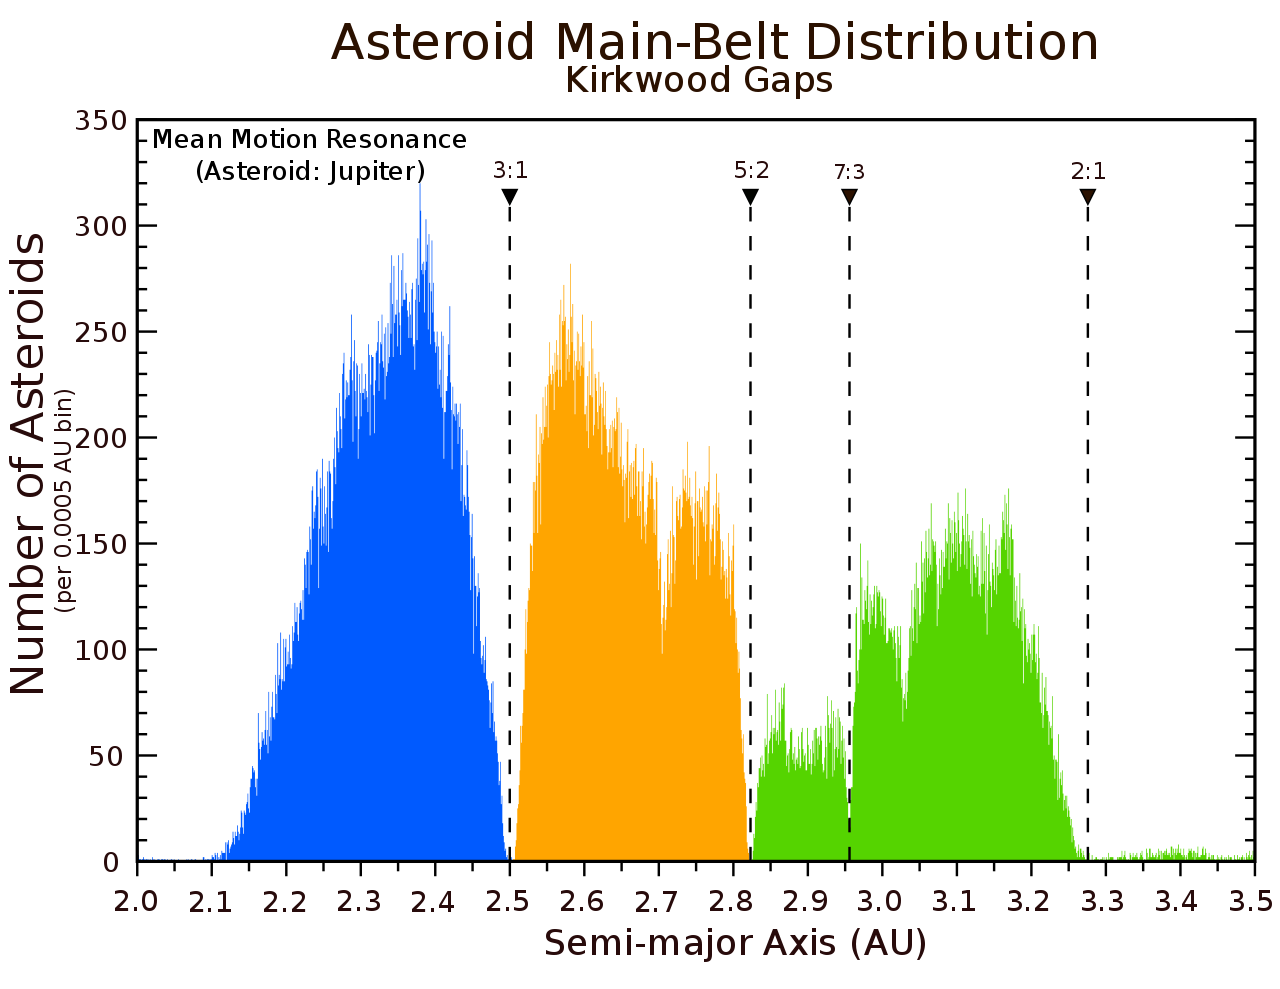
\includegraphics[scale=0.24]{figure/jupiter_resonances.png}
    \caption[Risonanze di moto medio con Giove.]{Istogramma che mostra i principali Kirkwood Gaps nella Main Belt. Sulle ascisse si trova il valore del semiasse maggiore, sulle ordinate il numero di asteroidi a una data distanza dal Sole. Le principali risonanze di moto medio sono indicate in alto. Per esempio la risonanza 3:1 è situata a una distanza tale per cui l'asteroide completa 3 orbite per ogni orbita completata da Giove. (JPL/Caltech)}
    \label{fig:jupiter_resonances}
\end{figure}

\begin{figure}
    \centering
    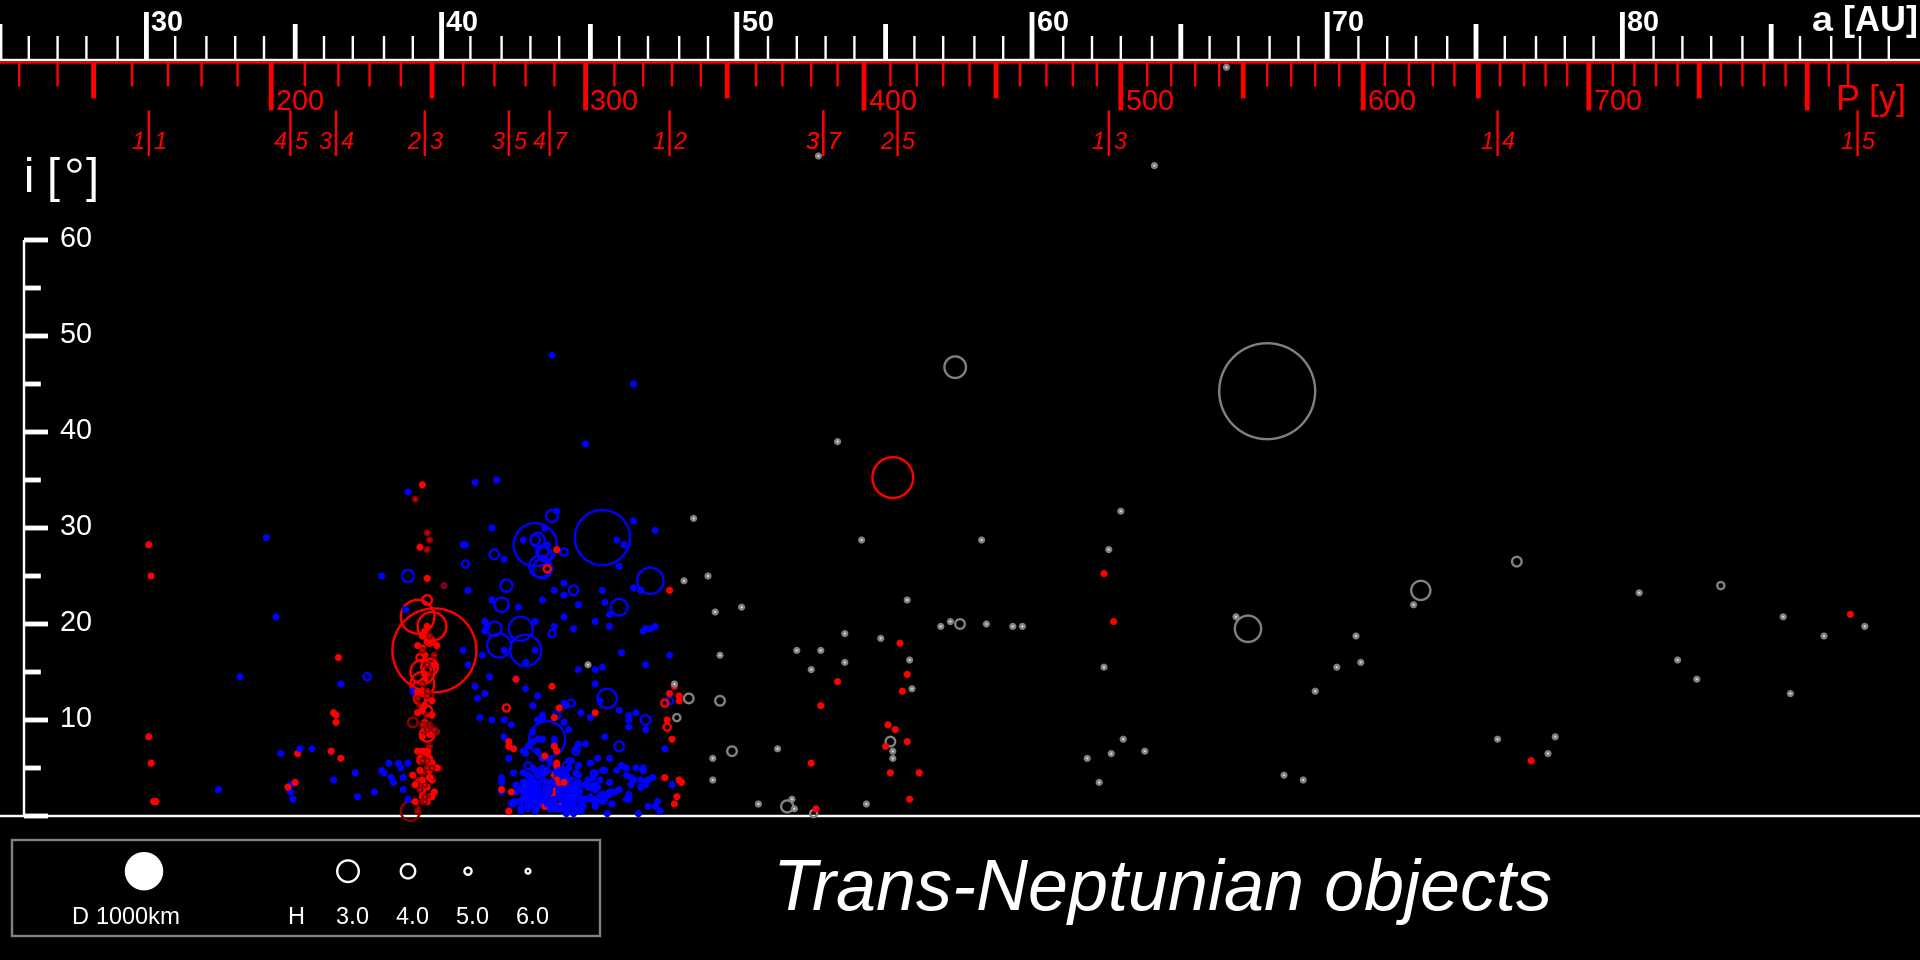
\includegraphics[width=\textwidth]{figure/neptune_resonances.png}
    \caption[Risonanze di moto medio con Nettuno.]{Istogramma che mostra la distribuzione degli oggetti trans-nettuniani. Sulle ascisse si trova il valore del semiasse maggiore (o il periodo), sulle ordinate il valore dell'inclinazione orbitale. Le principali risonanze di moto medio sono indicate in alto. (Wikipedia)}
    \label{fig:neptune_resonances}
\end{figure}

\subsection{Distribuzione e classificazione dinamica}
In questo paragrafo verrà decritta la classificazione in gruppi e famiglie.
La classificazione è riassunta nella \cref{tab:asteroid-classification} .\\
I corpi minori sono divisi in gruppi e famiglie in base alle loro caratteristiche orbitali. 
I gruppi sono associazioni dinamiche relativamente blande, mentre le famiglie sono dinamicamente più coese.

Per la classificazione è utile conoscere le definizioni analitiche di afelio e perielio di un'orbita:
\begin{equation}
    \begin{cases}
        Q=a(1+e) &\text{afelio}\\
        q=a(1-e) &\text{perielio}
    \end{cases}
\end{equation}

dove \textit{a} e \textit{e} sono rispettivamente il semiasse maggiore e l'eccentricità dell'orbita.

\paragraph*{Near Earth Objects}\label{sec:neo}
I Near Earth Objects (NEOs) rappresentano un gruppo eterogeneo di asteroidi (NEAs) e nuclei cometari estinti (NECs) che hanno orbite con un perielio minore di quello di Marte: $q<1.3$ AU. Si ritiene che i NEOs siano la principale fonte di meteoriti che arrivano sulla Terra.\\
In base alla relazione tra la loro orbita e quella della Terra sono catalogati in diversi sotto-gruppi: \textit{Atens} e \textit{Apollo} sono Earth Crossers (i.e. intersecano l’orbita della Terra), mentre gli \textit{Amors} si avvicinano alla Terra ma non intersecano mai la sua orbita. Gli Atens hanno un semiasse maggiore più piccolo di quello della Terra ($a<1$ AU) mentre gli Apollo hanno $a>1$ AU.


\begin{table}
    
    \begin{center}
    \resizebox{\linewidth}{!}{%
    
    \begin{tabular}{cccccc}
      \toprule
      \toprule
      \bf{Popolazione} & \bf{Famiglia/Gruppo} & \bf{a}     & \bf{q}     & \bf{Q}     & \bf{Commento} \\
      \midrule
      NEAs        &                 &       &       &       &           \\
                  & Atens           & $<1$  &              & $\geq 0.983$ & Earth Crossers     \\
                  & Apollos         & $>1$  & $\leq 1.017$ &              & Earth Crossers \\
                  & Amors           & $>1$  & $(1.017,1.3)$ &             &  \\
      \midrule
      Mars Crossers &               &       & $[1.3,1.67]$ &             &  \\
      \midrule
      \midrule
      \bf{Popolazione} & \bf{Famiglia/Gruppo} & \bf{a}     & \bf{e}     & \bf{i}     & \bf{Risonanze} \\
      \midrule
      Main Belt Asteroids &       &       &       &       &  \\
            & Hungarians & $[1.78,2.06]$ & $<0.18$ & $[16,34]$ & $[5:1, 4:1]$ \\
            & Inner MB & $[2.06,2.50]$ &       & $[18,32]$ & $[4:1,3:1]$ \\
            & Middle MB & $[2.50,2.82]$ &       &       & $[3:1,5:2]$ \\
            & Outer MB & $[2.82,3.28]$ &       &       & $[5:2,2:1]$ \\
            & Cybeles & $[3.28,3.70]$ & $<0.3$ & $<25$ & $[2:1,5:3]$ \\
            & Hildas & $\sim 3.97$ & $>0.07$ & $<20$ & $3:2$ \\
      \midrule
      Jupiter Trojans &       & $\sim 5.20$ &       &       & $1:1$ \\
      \midrule
      Centaurs &       & $[5.4,30]$ &       &       &  \\
      \midrule
      Neptune Trojans &       & $\sim 30$ &       &       & 1:1 Nep \\
      \midrule
      TNOs (o KBOs) &       & $>32$ &       &       & $[4:5, 2:3]$ Nep \\
            &       &       &       &       & $[3:5, 1:2]$ Nep \\
      \bottomrule
      \bottomrule
    \end{tabular}}%
    \end{center}
    \caption[Lista e definizioni delle principali popolazioni di asteroidi.]{Lista e definizioni dei principali gruppi e famiglie di asteroidi. Il semiasse maggiore $a$, il perielio $q$ e l'afelio $Q$ sono espressi in AU; l'inclinazione $i$ in gradi. $e$ è l'eccentricità. Le risonanze, dove non è indicato, si riferiscono all'orbita di Giove.}
    \label{tab:asteroid-classification}
\end{table}%
  

\paragraph*{Mars Crossers}
Come fa intendere il nome, i Mars Crossers (MCs) sono oggetti che intersecano l’orbita di Marte.\\
È stato mostrato che la popolazione dei Mars Crossers, che è circa 4 volte più grande di quella dei NEOs, è rifornita da risonanze diffusive nella Main Belt \citep{migliorini_origin_1998, morbidelli_numerous_1999, michel_population_2000, bottke_debiased_2002}, dalla regione chiamata “intermediate-source Mars-crossing region” o IMC.

\paragraph*{Main Belt Asteroids}
I Main Belt Asteroids (MBAs) sono asteroidi situati tra le orbite di Marte e Giove. La maggior concentrazione si trova tra 2.0 e 3.3 AU.\\
A causa delle risonanze orbitali dovute all’influenza gravitazionale di Giove, si vengono a creare molti gruppi, sotto-gruppi e famiglie. Di seguito sono riportati i più popolosi.

\qquad \textit{Hungaria}: prendono il nome da (434) Hungaria. Hanno un semiasse maggiore tra 1.78 e 2.06 AU, un’eccentricità minore di 0.18 e un’inclinazione tra 16° e 34°. 

\qquad \textit{Inner Main Belt}: hanno un semiasse maggiore tra 2.06 e 2.50 AU, limiti definiti dalle risonanze di moto medio 4:1 e 3:1.

\qquad \textit{Middle Main Belt}: hanno un semiasse maggiore tra 2.50 e 2.82 AU. I limiti sono definiti dalle risonanze di moto medio 3:1 e 5:2.

\qquad \textit{Outer Main Belt}: hanno un semiasse maggiore tra 2.82 e 3.28 AU. All’interno del gruppo troviamo le famiglie \textit{Koronis}, \textit{Eos} e \textit{Themis}.

\qquad \textit{Cybele}: hanno un semiasse maggiore tra 3.28 e 3.70 AU. Prendono il nome da (65) Cybele.

\qquad \textit{Hilda}: hanno un semiasse maggiore medio tra 3.70 e 4.20 AU. Prendono il nome da (153) Hilda.

\paragraph*{Jupiter Family Comets}
Le comete sono divise in due gruppi: comete a lungo periodo e comete a corto periodo.\\
Le comete a corto periodo della Jupiter Family, chiamate in questo modo poiché la loro orbita è controllata dall'interazione gravitazionale con Giove, hanno un periodo orbitale $< 20$ anni. 
Dato che i valori tipici dell'inclinazione sono vicini al piano dell'eclittica, si pensa che le comete a corto periodo provengano dalla Kuiper Belt, una grande riserva di piccoli corpi ghiacciati che si trova oltre Nettuno. A causa di collisioni e/o perturbazioni gravitazionali alcuni oggetti della Kuiper Belt riescono a fuggire dalla stessa e a dirigersi verso il Sistema Solare interno.

\paragraph*{Centaurs}
I Centauri sono oggetti che orbitano tra Giove e Nettuno ($5.4<a<30$ AU), ma non hanno ancora una definizione dinamica univoca.\\
Studi dinamici delle loro orbite indicano che i Centauri sono probabilmente degli oggetti con caratteristiche orbitali intermedie tra quelli della Kuiper Belt e le JFCs.\\
Sono probabilmente più simili a comete che ad asteroidi e uno di questi, Chirone, è stato osservato avere attività cometaria.

\paragraph*{Trans Neptunian Objects}
Sono oggetti con $a\geq 40$ AU e sono divisi nei seguenti gruppi:

\qquad \textit{Kuiper Belt Objects}: si trovano tra 41 e 47 AU. A sua volta si divide nei sotto-gruppi dei \textit{Plutinos}, in risonanza 3:2 con Nettuno come Plutone, e dei \textit{Cubewanos}, conosciuti come i classici KBOs.

\qquad \textit{Scattered-Disk Objects (SDOs)}: hanno orbite con un grande semiasse e molto ellittiche. La spiegazione dei valori di questi parametri è ancora incerta: probabilmente sono dovuti a un’interazione con Nettuno e/o a espulsioni primordiali durante le migrazioni planetarie.

\qquad \textit{Oort Cloud Objects (OCOs)}: la Oort Cloud è un guscio sferico di oggetti ghiacciati, di cui non si ha evidenza diretta perché troppo lontano e scuro ma ipotizzato come luogo di origine delle comete a lungo/lunghissimo periodo. Si troverebbe tra circa 50000 e 100000 AU.

\subsection{Effetto Yarkovsky}
L’effetto Yarkovsky è una forza percepita da un corpo dovuta all’emissione anisotropa di fotoni termici, che trasportano momento. La sua influenza è più significativa per meteoroidi e piccoli asteroidi, da $10\; cm$ a $10\; km$ di diametro \citep{vokrouhlicky_yarkovsky_2015}.\\
L’effetto fu scoperto da Ivan Osipovich Yarkovsky, che notò come il riscaldamento diurno di un oggetto rotante nello spazio causasse una piccola forza sull’oggetto che avrebbe avuto effetti a lungo termine sulla sua orbita.

L’effetto è dovuto a due componenti:

\paragraph*{Effetto diurno}
Su un corpo che ruota illuminato dal Sole la superficie si scalda durante il giorno, mentre si raffredda durante la notte. Di conseguenza la superficie tende a essere più calda nel tardo pomeriggio e ad inizio sera, mentre è più fredda nelle altre fasi della giornata. L’emisfero caldo emette quindi più radiazione di quello freddo: la differenza della pressione di radiazione induce una forza la cui direzione dipende dalla rotazione dell’oggetto. Per oggetti rotanti in modo progrado, questa forza è nella direzione della loro orbita e il semiasse maggiore, nel lungo periodo, tende ad aumentare. Situazione opposta per gli oggetti che ruotano in modo retrogrado.

\paragraph*{Effetto stagionale}
Questa seconda tipologia tiene conto del fatto che nel corso di un anno uno dei due emisferi dell’asteroide risulta maggiormente esposto alla radiazione solare rispetto all’altro. Per oggetti rotanti, l’effetto stagionale aumenta con l’inclinazione assiale. Esso domina solo se l’effetto diurno è abbastanza piccolo \citep{Vokrouhlicky_1999}.
L’effetto stagionale potrebbe avvenire per:

\begin{itemize}
    \item rotazione molto veloce
    \item piccole dimensioni dell’oggetto
    \item inclinazione assiale vicina a 90°
\end{itemize}

Anche questo effetto ha ripercussioni sul semiasse maggiore e nell'ordine dei milioni di anni può portare un asteroide dalla Main Belt al Sistema Solare interno.

\begin{figure}[!h]
    \centering
    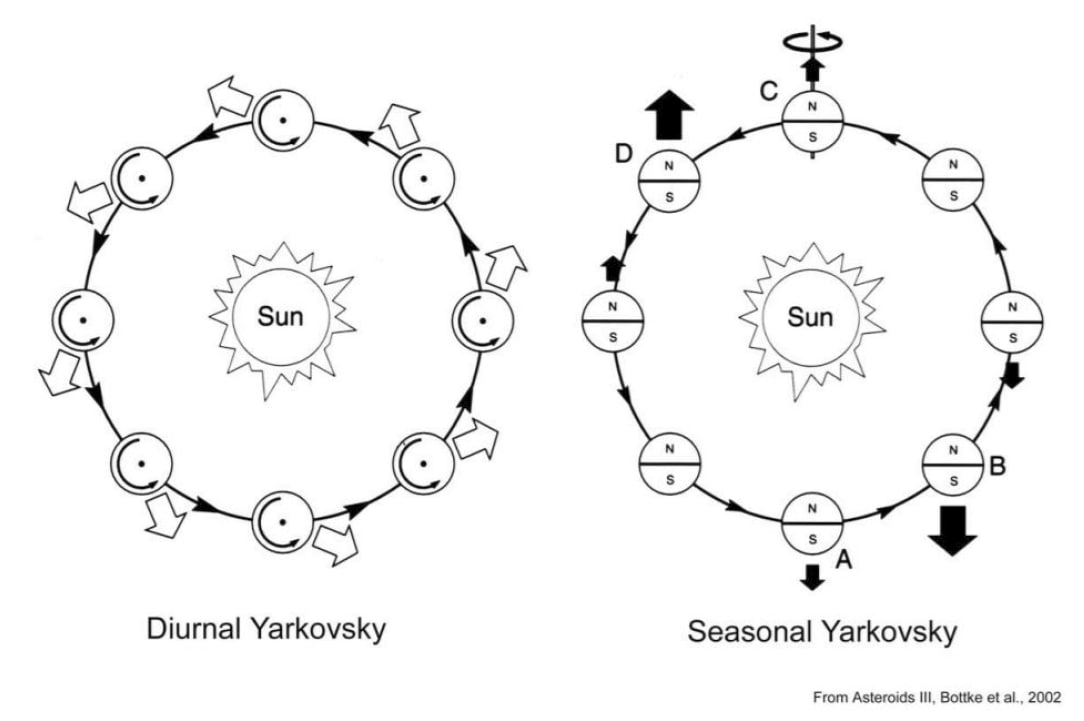
\includegraphics[scale=0.38]{figure/yark.jpg}
    \caption[Visualizzazione dell'effetto Yarkovsky diurno e stagionale.]{Visualizzazione dell'effetto Yarkovsky diurno (a sinistra) e stagionale (a destra). \citep{bottke_yarkovsky_2002}}
    \label{fig:yark}
\end{figure}

\paragraph*{Effetto YORP}
L’effetto Yarkovsky-O'Keefe-Radzievskii-Paddack (YORP) è un variazione al secondo ordine dell’effetto Yarkovsky, sempre dovuta alla radiazione solare assorbita e successivamente riemessa dal corpo, che causa l’aumentare o il diminuire della velocità di rotazione (o spin) di un piccolo corpo, come un asteroide.\\
Sul lungo periodo, l'inclinazione e il tasso di rotazione dell'oggetto possono variare in modo casuale, in modo caotico o regolare, a seconda di molti fattori.

\section{Potentially Hazardous Asteroids}\label{sec:pha}
Tra i NEO esiste una categoria di oggetti che riveste un ruolo importante: sono gli asteroidi potenzialmente pericolosi, Potentially Hazardous Asteroids (PHA). Rientrano in questa categoria tutti gli oggetti la cui minima distanza all'intersezione dell'orbita terrestre (Minimum Orbit Intersection Distance - MOID) è inferiore a 0.05 AU e la cui magnitudine assoluta H è minore di 22. Sono quindi quegli asteroidi che se impattassero con la Terra provocherebbero danni su larga scala, anche globale. A oggi si conoscono più di 2500 PHA, la maggior parte dei quali sono della famiglia Apollo, e ogni giorno vengo aggiunti o rimossi oggetti sulla base di nuovi risultati dei parametri orbitali.\\
La determinazione dell'orbita avviene sulla base delle osservazioni disponibili ed è definita da sei parametri orbitali, influenzati da diversi fattori. Quindi non si può determinare immediatamente con sufficiente accuratezza l'orbita ma servono osservazioni costanti nel tempo.\\
Al momento della scoperta di un PHA si calcola l'orbita per i successivi 100 anni. Si possono determinare in tal modo i passaggi ravvicinati (fly-by) che l'asteroide avrà con la Terra e, conoscendo la regione di incertezza, la probabilità di collisione con la stessa.

\begin{figure}
    \centering
    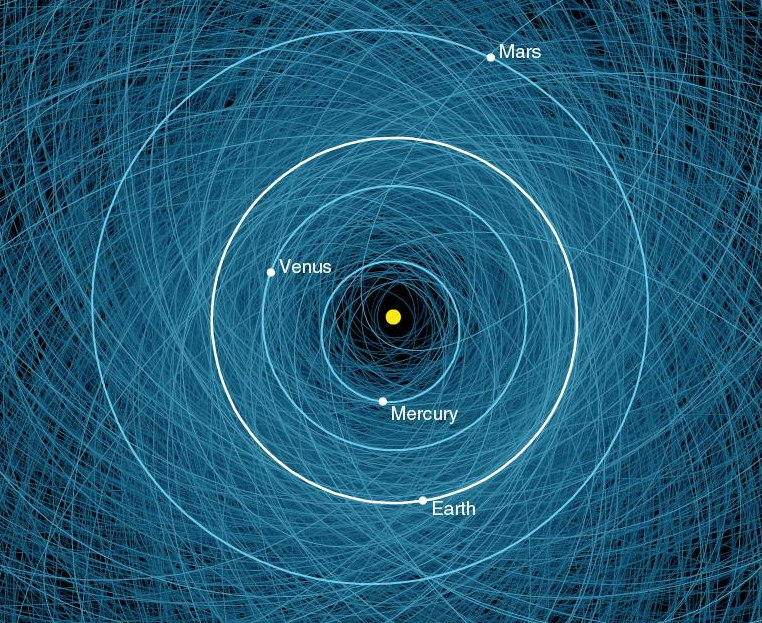
\includegraphics[scale=0.35]{figure/pha_map.jpg}
    \caption[Visualizzazione delle orbite dei PHA conosciuti.]{Visualizzazione delle orbite dei PHA conosciuti. Si nota come la zona intorno all'orbita terrestre sia molto popolata. (NASA/JPL-Caltech)}
    \label{fig:pha_map}
\end{figure}

I PHA con una probabilità non nulla di impatto con la Terra nei futuri 100 anni vengono inseriti nella Sentry Risk Table\footnote{\href {https://cneos.jpl.nasa.gov/sentry/}{https://cneos.jpl.nasa.gov/sentry/} }, un sistema informatico gestito dal CNEOS (Center for Near-Earth Object Studies).\\
Oltre alla probabilità di collisione e alcune caratteristiche dell’oggetto (magnitudine assoluta, diametro) vengono riportati i valori dell’asteroide sulla Scala Torino e Scala Palermo. Queste sono due classificazioni che permettono di quantificare il pericolo associato a ogni asteroide: la Scala Torino è stata pensata per la comunicazione al pubblico, la Scala Palermo è più tecnica e viene usata direttamente dagli astronomi.


\chapter{Spettroscopia}\label{ch:ch_2}

\section{Introduzione}
Lo studio della mineralogia superficiale di singoli asteroidi o di gruppi di asteroidi può fornire i dati per migliorare la nostra comprensione della loro origine ed evoluzione. La superficie degli asteroidi può essere studiata dall'interpretazione delle proprietà osservabili per determinare la presenza, l'abbondanza e la composizione mineralogica.\\
La spettroscopia di riflettanza nel visibile (VIS) e nell'infrarosso (IR) viene ampiamente usata per determinare la composizione degli asteroidi poiché può caratterizzare la composizione superficiale della maggior parte dei tipi di asteroidi. Le caratteristiche diagnostiche negli spettri, che derivano da transizioni elettroniche e vibrazionali all'interno dei minerali e delle molecole, sono riscontrabili nell'intervallo di frequenza $0.35-2.50\,\mu m$.\\
I minerali più importanti presenti negli spettri degli asteroidi sono: olivine, pirosseni, metalli ferro-nichel (Fe-Ni), feldspati e fillosilicati idrati e composti organici. Poiché i parametri spettrali dei diversi assorbimenti (e.g. la posizione delle bande e il rapporto tra esse) sono legati a una specifica composizione del singolo minerale, l'analisi spettrale della superficie degli asteroidi è in grado, nella maggior parte dei casi, di rilevare le firme mineralogiche caratteristiche di una particolare specie. La possibilità di rilevare un'intensità dipende dall'abbondanza della particolare specie, in modo che la forza dell'intensità possa essere rilevata sopra il rumore dello spettro. In spettri di alta qualità possono essere anche determinate la composizione e le relative abbondanze. Per questi motivi l'analisi degli spettri può fornire una varietà di dati sulla composizione della superficie degli asteroidi.\\
Ogni asteroide ha una composizione, forma, dimensione e altre proprietà fisiche uniche, benché vengano raggruppati in un paio di dozzine di classi spettrali. Un impressionante numero di informazioni sulla composizione degli asteroidi è stato raccolto attraverso osservazioni da Terra e missioni spaziali. Tuttavia, il livello di dettaglio che si può ottenere attraverso lo studio delle meteoriti nei laboratori sulla Terra è incomparabile. Pertanto, collegare le meteoriti agli asteroidi è fondamentale per individuare le moltissime informazioni compositive contenute nelle asteroidi. Stabilire queste connessioni asteroide-meteorite non è banale perché gli spettri raramente corrispondono direttamente uno a uno. Gli spettri degli asteroidi sono campionati su una superficie che va da metri a centinaia di chilometri, mentre quelli delle meteoriti sono effettuate su un campione piccolo e localizzato. Gli spettri, inoltre, non contengono solo informazioni sulla composizione, ma dipendono da fattori quali la granulometria delle particelle sulla superficie dell'asteroide o del campione di meteorite, l'angolo di fase dell'osservazione e la temperatura \citep{demeo_connecting_2022}. In aggiunta, le superfici degli asteroidi sono alterate dall'ambiente spaziale, un processo chiamato space weathering che verrà brevemente discusso nella \cref{sec:space_weathering}.



\section{Spettri degli asteroidi}
Il flusso incidente che arriva sulla superficie di un asteroide è diviso in due contributi: la parte riflessa e la parte assorbita, il cui rapporto dipende dall'albedo. La parte assorbita riscalda la superficie del corpo. Questo emette, di conseguenza, radiazione di corpo nero determinata dalla temperatura raggiunta. Quindi la Terra riceve sia il flusso "solare" riflesso dall'oggetto che la radiazione di corpo nero.\\
Negli spettri degli asteroidi la radiazione solare riflessa domina nel range che va dall'ultravioletto (UV) al vicino infrarosso (NIR): $0.35-2.50\,\mu m$; mentre il contributo della radiazione di corpo nero dell'asteroide diventa rilevabile a lunghezze maggiori ($2.5-5.0\,\mu m$).

\section{Tipi tassonomici}
La tassonomia è la classificazione degli oggetti in categorie definite da alcuni parametri caratterizzanti. Sin dagli anni '70 diversi autori hanno creato diverse classi tassonomiche basandosi su proprietà osservabili.\\
La prima classificazione tassonomica più utilizzata è stata quella di \citet{tholen_asteroid_1984}, basata su più di 400 spettri ricavati dalla Eight-Color Asteroid Survey (ECAS), nel range spettrale $0.3-1.1\,\mu m$. Dagli spettri ECAS si possono distinguere undici classi spettrali: A, B, C, D, F, G, Q, R, S, T e V.\\
In seguito vennero sviluppate altre classificazioni tassonomiche, tra cui quella di Bus e Binzel \citep{bus_phase_2002-1, bus_phase_2002}, che hanno derivato la loro classificazione da dati spettrofotometrici recenti. Attualmente la classificazione di Bus e Binzel è la più utilizzata.

\subsection{Tassonomia di Tholen}
Ognuna delle classi di Tholen separa gli asteroidi in diverse classi secondo riflettività e albedo visuali (nel visibile) simili. Sebbene non venga usato nessun criterio mineralogico nel definire le classi, la tassonomia può essere usata per derivare la caratterizzazione mineralogica di ogni asteroide nelle varie classi.\\
Di seguito descriveremo brevemente le principali caratteristiche di ogni classe della tassonomia di Tholen e la loro relazione con le meteoriti. 

\paragraph*{Classe A}
Gli asteroidi di tipo A mostrano una forte decrescita nella riflettanza attorno a $0.7\,\mu m$, relativa a composti metallici, e un forte banda di assorbimento centrata attorno a $1\,\mu m$ e nessun assorbimento rilevante a $2\,\mu m$ (caratteristica dei pirosseni).\\
Sono asteroidi molto rari, situati nella Main Belt interna. Si ritiene che questi oggetti siano frammenti del mantello differenziato di corpi progenitori di dimensioni maggiori.\\
Le meteoriti analoghe sono le acondriti a olivina e/o pallasite.

\paragraph*{Classe Q}
È una classe di oggetti molto scarna, i pochi corpi di questo tipo sono NEO ma nessuno appartiene alla Main Belt. Un ottimo rappresentante della classe è (1862) Apollo. Lo spettro è fortemente arrossato attorno a $0.7\,\mu m$ e ha due forti assorbimenti a $1$ e $2\,\mu m$, caratteristiche proprie di un mix di olivine e pirosseni.\\
Questi spettri sono simili a quelli delle condriti ordinarie (CO), che rappresentano circa l'80\% delle meteoriti trovate sulla superficie terrestre. Ciò indicherebbe che gli asteroidi di tipo Q siano i progenitori di queste meteoriti e quindi dovrebbero essere molto numerosi, in contrasto con le osservazioni.

\begin{figure}[!h]
\centering
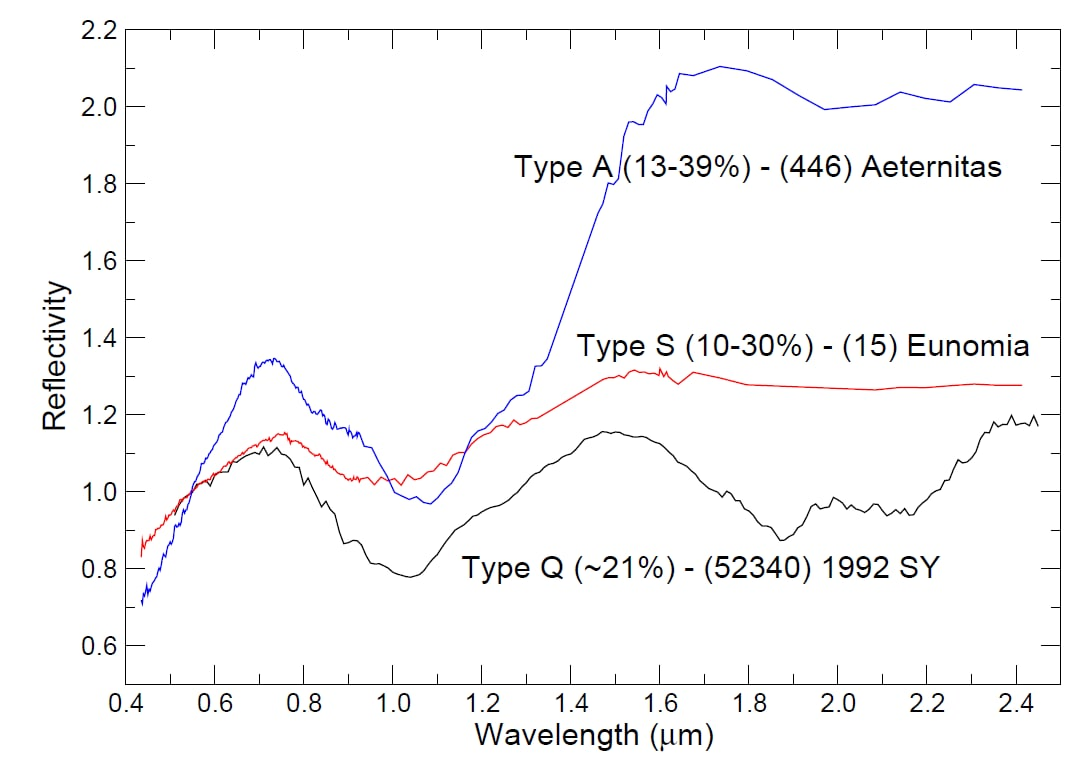
\includegraphics[scale=0.3]{figure/spettro_qsa.jpg}
\caption[Esempio di spettri di tipo Q, S e A.]{Esempio di spettri di tipo Q, S e A. Gli spettri sono normalizzati a $0.55\,\mu m$. Tra parentesi è riportato il range di albedo in percentuale. \citep{magrin_spectroscopic_nodate}}
\label{spettro_qsa}
\end{figure}

\paragraph*{Classe S}
Rappresenta la seconda classe più numerosa ed è caratterizzata da spettri con una pendenza ripida attorno a $0.7\,\mu m$ e assorbimenti moderati attorno a $1$ e $2\,\mu m$ (dovuti a olivina e pirossene). La loro albedo varia tra $0.1$ e $0.3$. Lo spettro tipico degli asteroidi di tipo S indica la presenza di un mix di olivine, pirosseni e metalli Fe-Ni, in particolare di silicati: ciò li rende i corpi progenitori più probabili per le condriti ordinarie.\\
A causa dei limiti della classificazione Tholen all’interno del gruppo S sono stati identificati oggetti di composizione molto diversa tra loro. Sono stati pertanto introdotti diversi sottogruppi, definiti in base alle diverse composizioni e storie evolutive degli asteroidi.\\
Gli asteroidi di tipo S sono situati principalmente nella Main Belt interna e diventano più rari spostandosi verso l'esterno.

\paragraph*{Classe V}
Questa classe fu proposta per (4) Vesta. Il suo spettro è caratterizzato da forti assorbimenti centrati vicino a $1$ e $2\,\mu m$, dovuti ai pirosseni.\\
All'incirca il 6\% degli asteroidi della Main Belt rientra all'interno di questo gruppo. La maggior parte degli asteroidi di tipo V, noti come vestoidi, orbita nelle vicinanze di Vesta, il che suggerisce che siano dei suoi frammenti generatisi in seguito a impatti con altri corpi. Alcuni NEA sono risultati essere vestoidi: ciò dimostra l'efficacia dei meccanismi di trasporto degli asteroidi dalla Main Belt alle regioni del Sistema Solare interno.

\begin{figure}[!h]
    \centering
    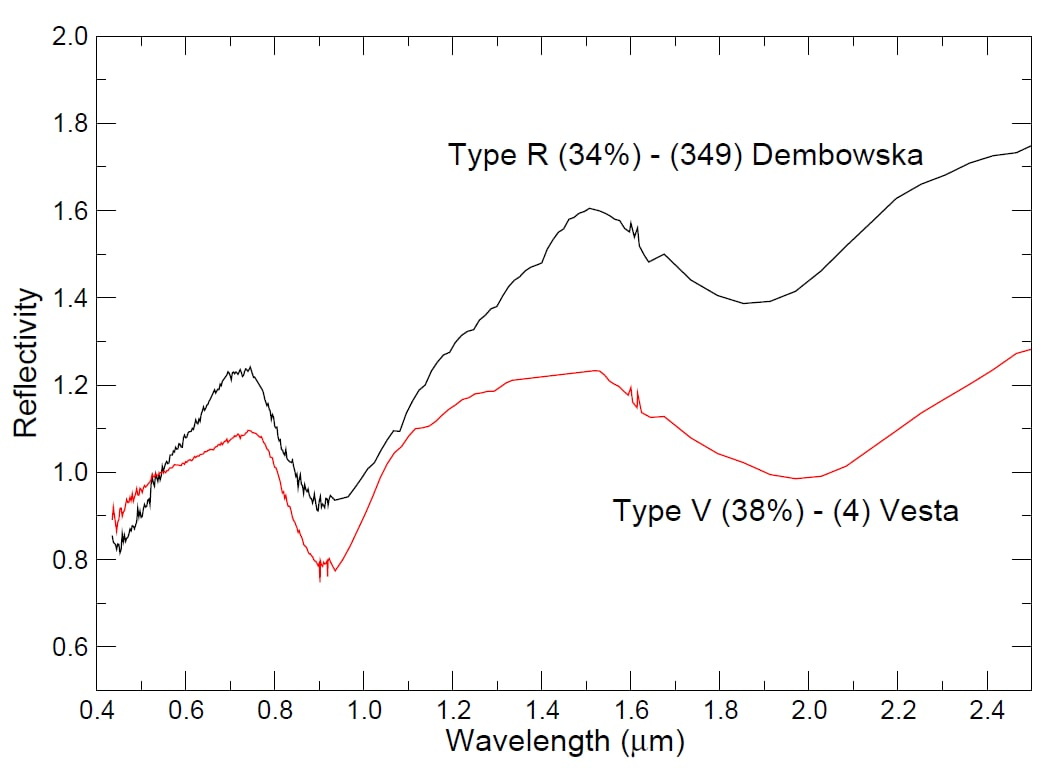
\includegraphics[scale=0.3]{figure/spettro_rv.jpg}
    \caption[Esempio di spettri di tipo V e R.]{Esempio di spettri di tipo V e R. Gli spettri sono normalizzati a $0.55\,\mu m$. Tra parentesi è riportato il range di albedo in percentuale. \citep{magrin_spectroscopic_nodate}}
    \label{spettro_rv}
\end{figure}

\paragraph*{Classe R}
Questa classe fu inizialmente proposta unicamente per (349) Dembowska. Il suo spettro mostra forti assorbimenti a $1$ e $2\,\mu m$, simili a quelli di Vesta. Dembowska, a differenza di Vesta, presenta caratteristiche allargate verso lunghezze d'onda maggiori, mentre l'assorbimento a $2\,\mu m$ è più stretto e centrato su lunghezze d'onda minori.\\
Le caratteristiche spettrali indicano la presenza di olivine e pirosseni (circa in eguali quantità) e pochi metalli. 

\paragraph*{Classe C}
Gli asteroidi di tipo C sono caratterizzati da albedo molto basse ($<0.10$) e da una composizione superficiale costituita per gran parte da carbonio. Sembrano pertanto essere i corpi progenitori più probabili per le condriti carbonacee. Contiene infatti circa il 75\% degli asteroidi noti. Questi oggetti dominano nelle regioni esterne della Main Belt, dove compongono l'80\% di tutta la popolazione, ma diventano più rari spostandosi verso l'interno.\\

\begin{figure}[!h]
    \centering
    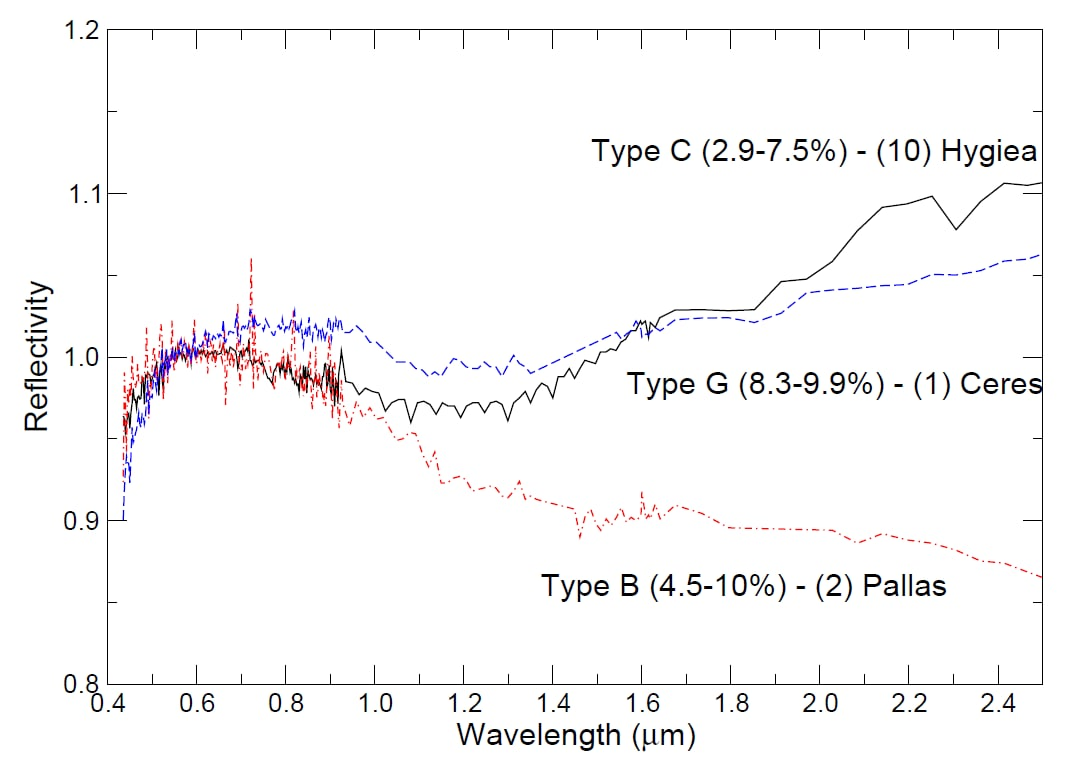
\includegraphics[scale=0.3]{figure/spettro_bgc.jpg}
    \caption[Esempio di spettri di tipo B, G e C.]{Esempio di spettri di tipo B, G e C. Gli spettri sono normalizzati a $0.55\,\mu m$. La scala verticale è ampliata per rendere apprezzabili le differenze tra le classi. Tra parentesi è riportato il range di albedo in percentuale. \citep{magrin_spectroscopic_nodate}}
    \label{spettro_bgc}
\end{figure}

Gli asteroidi di tipo C non presentano alcuna caratteristica attorno a $0.4\,\mu m$ ma hanno intensità di assorbimento differenti nell'UV. All'interno di questa classe sono state introdotte le sottoclassi C, B, F, G e P.\\
La classe P non ha assorbimenti nell'UV, la classe F ne ha uno debole, B e C leggermente più intenso e la classe G ha l'assorbimento UV più intenso di tutto il gruppo C. La classe B ha uno spettro da piatto a leggermente blu mentre la classe C da piatto a leggermente rosso. \citet{bell_asteroids_1989} ha proposto un modello per interpretare le diversità nel gruppo C: le classi B, F e G sarebbero il risultato di un'alterazione metamorfica di un progenitore di classe C. La classe P, che si trova principalmente nella parte esterna della Main Belt, si pensa sia costituita da materiale primitivo contenente una gran quantità di materiale organico e potrebbe essere una classe di transizione tra C e gli oggetti molto primitivi della classe D.\\
Circa due terzi degli oggetti del gruppo C appaiono idratati, dall'analisi dello spettro attorno a $3\,\mu m$ e nella regione del visibile, probabilmente perché sono stati scaldati al punto che acqua liquida è entrata in contatto con il materiale circostante.

\paragraph*{Classe D}
Gli spettri degli asteroidi di classe D sono generalmente senza caratteristiche particolari, tendenti leggermente verso il rosso attorno a $0.55\,\mu m$ e molto rossi dopo $0.55\,\mu m$. Hanno inoltre albedo molto basse ($\leq 0.05$).\\
Sono situati nella Main Belt esterna e tra i Troiani di Giove, di cui costituiscono il 60\% della popolazione totale \citep{VILAS1985503}.

\begin{figure}[!h]
    \centering
    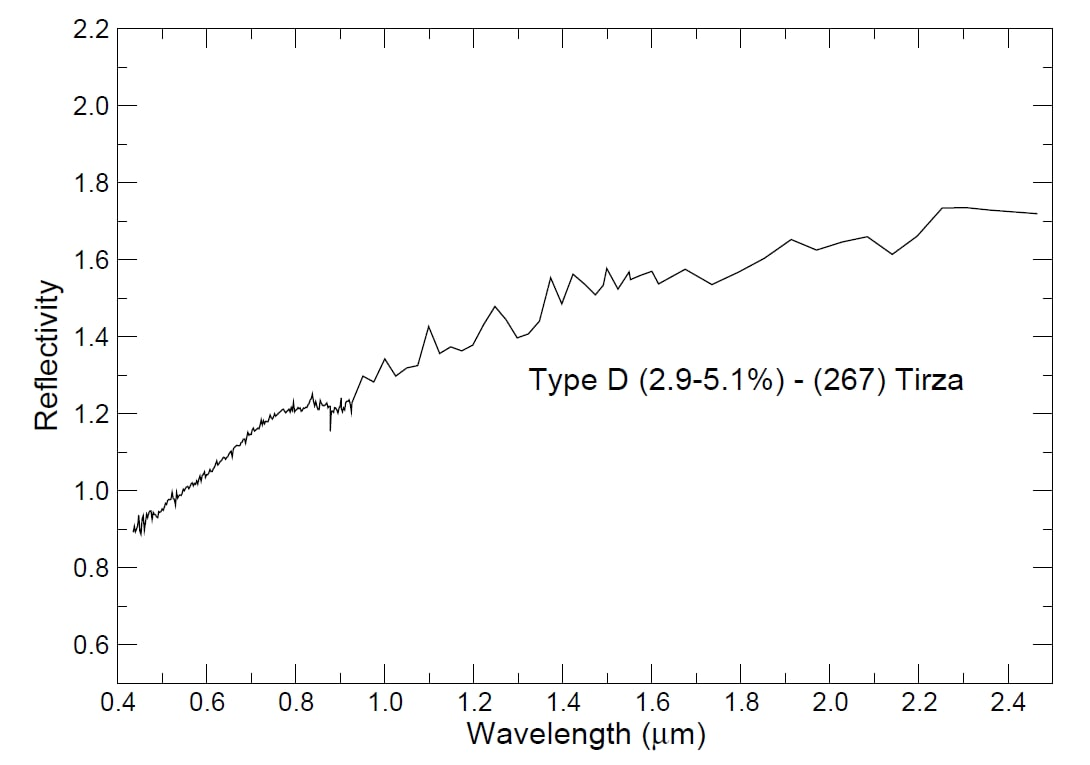
\includegraphics[scale=0.3]{figure/spettro_d.jpg}
    \caption[Esempio di spettro di tipo D.]{Esempio di spettro di tipo D. Lo spettro è normalizzato a $0.55\,\mu m$. Tra parentesi è riportato il range di albedo in percentuale. \citep{magrin_spectroscopic_nodate}}
    \label{spettro_d}
\end{figure}

\paragraph*{Classe M}
Si tratta del terzo gruppo più numeroso. Gli spettri sono caratterizzati da un leggero arrossamento e senza particolari caratteristiche. Gli asteroidi di questa classe hanno albedo comprese tra $0.1$ e $0.2$. I dati suggeriscono che la composizione sia principalmente ferro e nichel, suggerendo che questi oggetti siano i nuclei metallici differenziati di oggetti più grandi andati distrutti. Si ritengono essere quindi i progenitori delle meteoriti metalliche.

\begin{figure}[h]
    \centering
    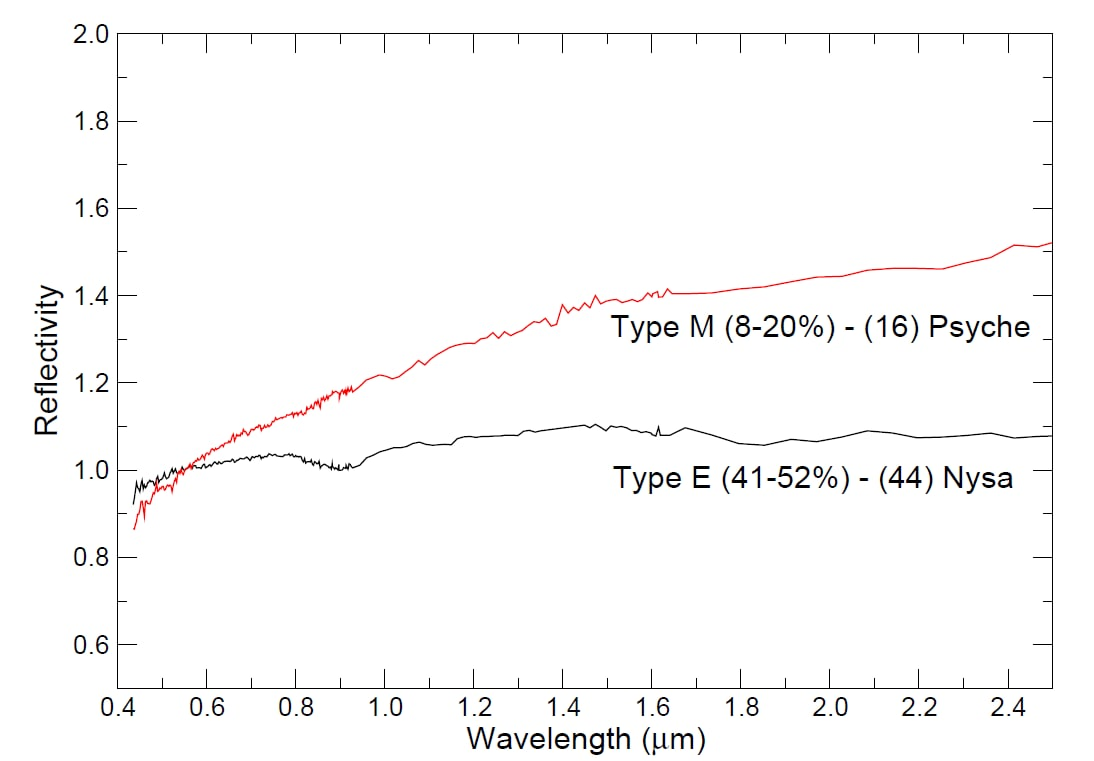
\includegraphics[scale=0.3]{figure/spettro_em.jpg}
    \caption[Esempio di spettri di tipo E e M.]{Esempio di spettri di tipo E e M. Gli spettri sono normalizzati a $0.55\,\mu m$. Tra parentesi è riportato il range di albedo in percentuale. \citep{magrin_spectroscopic_nodate}}
    \label{spettro_em}
\end{figure}

\paragraph*{Classe E}
Gli asteroidi di classe E hanno uno spettro senza caratteristiche, molto simile a quello della classe M. Si differenziano da questi ultimi per via della loro elevata albedo, superiore a $0.3$. La composizione superficiale dovrebbe essere costituita da silicati poveri di ferro, come enstatite e feldspato.\\
Il gruppo degli Hungaria contiene la metà degli asteroidi di classe E noti. Si crede che alcuni NEO di questo gruppo siano i corpi progenitori delle aubriti, una sottoclasse delle meteoriti acondriti.

\paragraph*{Classe T}
Gli asteroidi di classe T sono molto rari e hanno albedo molto basse ($\leq 0.1$), con spettri leggermente rossi vero $0.85\,\mu m$. Si ritiene che siano composti da materiale carbonaceo fortemente
alterato (o termicamente o dall'azione dell'acqua).

\begin{figure}[!h]
    \centering
    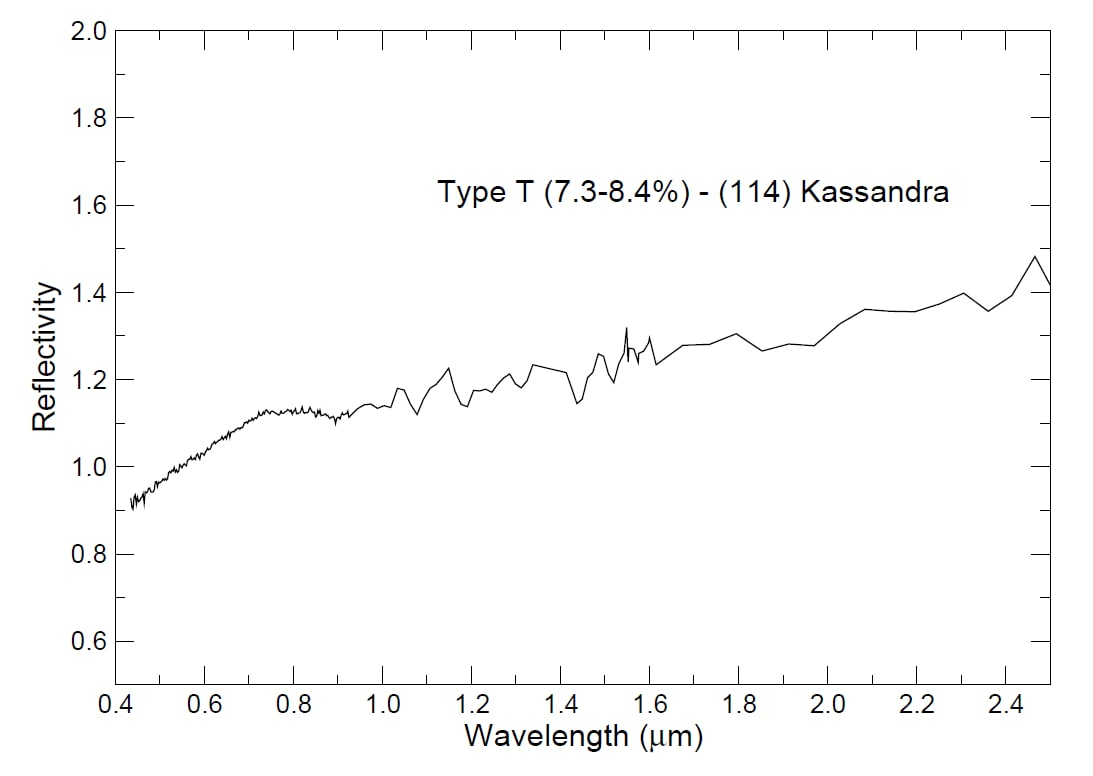
\includegraphics[scale=0.3]{figure/spettro_t.jpg}
    \caption[Esempio di spettro di tipo T.]{Esempio di spettro di tipo T. Lo spettro è normalizzato a $0.55\,\mu m$. Tra parentesi è riportato il range di albedo in percentuale. \citep{magrin_spectroscopic_nodate}}
    \label{spettro_t}
\end{figure}

\subsection{Tassonomia di Bus}
I dati della SMASSII\footnote{\href{http://smass.mit.edu/smass.html}{http://smass.mit.edu/smass.html}} (Small Main-Belt Asteroid Spectroscopic Survey) hanno fornito le basi per una nuova tassonomia. \citet{bus_phase_2002, bus_phase_2002-1} hanno costruito il loro sistema di classificazione basandosi sulle tassonomie pre-esistenti. In particolare hanno definito tre gruppi principali: S-, C- e X-complex, corrispondenti alle definizioni classiche dei tipi S, C e X. Di conseguenza sono state definite 26 classi sulla base della presenza o assenza di assorbimenti, quando presenti, e delle pendenze degli spettri. Di queste 26 classi, 12 hanno una designazione a una lettera: A, B, C, D, K, O, Q, R, S, T, V e X. Una nuova classe, la L, è stata introdotta per descrivere gli oggetti con una pendenza molto ripida nell'UV, vicino a $0.75\,\mu m$, ma con uno spettro piatto oltre i $0.75\,\mu m$. Asteroidi con caratteristiche intermedie sono associati a classi multi-lettera: Cb, Cg, Cgh, Ch, Ld, Sa, Sk, Sl, Sq, Sr, Xc, Xe, e Xk. I membri delle classi Cgh- e Ch- hanno spettri contenenti un assorbimento a $0.7\,\mu m$ legato all'idratazione.\\
Un nuovo asteroide può quindi venire facilmente classificato all’interno di una di queste classi solamente sulla base delle sue caratteristiche spettrali. Successivamente, \citet{demeo_extension_2009} ha coinvolto nella classificazione anche la regione infrarossa. Di seguito un riassunto degli spettri medi per ogni classe tassonomica secondo la tassonomia Bus-DeMeo.

\begin{figure}[!ht]
    \centering
    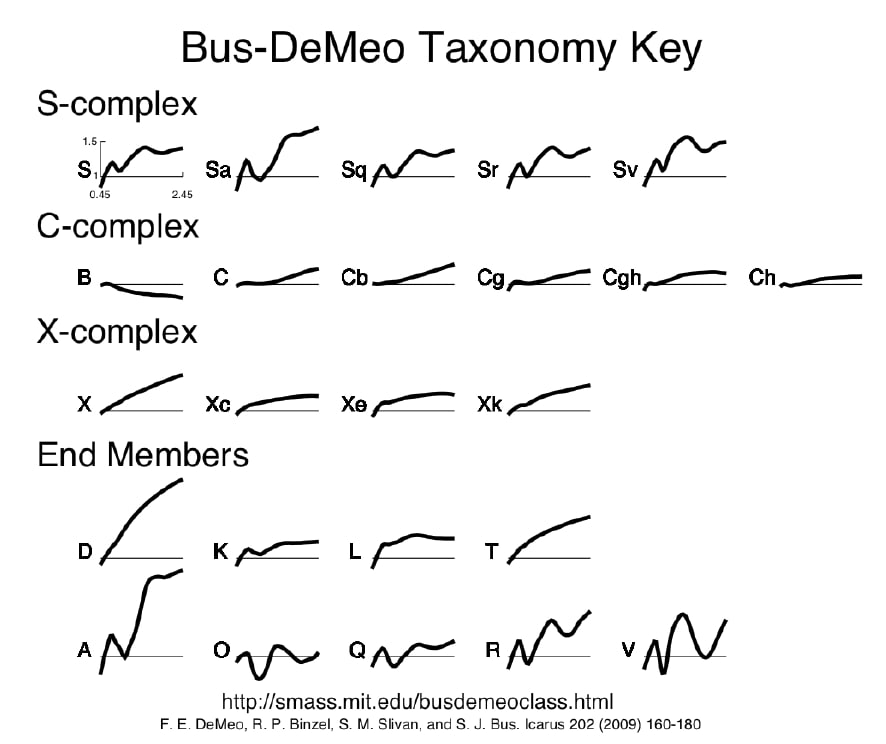
\includegraphics[scale=0.44]{figure/spettro_bus.jpg}
    \caption[Spettri dei tipi tassonomici introdotti da Bus e Binzel.]{Spettri dei tipi tassonomici introdotti da Bus e Binzel. \citep{demeo_extension_2009}}
    \label{spettro_bus}
\end{figure}

\section{Space weathering}\label{sec:space_weathering}
Lo space weathering (SW) è un termine che indica dei processi riguardanti i corpi senza atmosfera nel Sistema Solare. Questi processi includono irraggiamento da ioni solari (vento solare, flares, espulsioni di particelle energetiche), raggi cosmici galattici, elettroni, raggi UV e X e bombardamenti da parte di micrometeoriti. Le alterazioni superficiali dovute a questi effetti variano non solo in funzione della composizione superficiale ma anche della zona di Sistema Solare in cui si trovano gli oggetti affetti da SW.\\
La Luna è l'oggetto senza atmosfera più studiato e di cui si conoscono meglio gli effetti di SW \citep{gold_lunar_1955, hapke_space_2001}. 
%Il principale responsabile è ferro metallico in nanofase ($npFe^0$) che è prodotto dal 
La causa principale è il bombardamento del vento solare \citep{keller_nature_1997} e il suo effetto è quelli di rendere più arrossati gli spettri di riflettanza e scurire la regione del visibile-vicino infrarosso (VIS-NIR).\\
Per quanto riguarda gli asteroidi, lo SW è sempre stato considerato per cercare di spiegare possibili corrispondenze (o discrepanze) tra le classi tassonomiche e le meteoriti. Il problema più studiato è quello che concerne la possibilità che gli asteroidi di tipo S (S-type) siano i corpi progenitori delle condriti ordinarie (OC). %Numerosi studi si sono concentrati sul confronto della mineralogia degli S-type con le OC, giungendo alla conclusione che potrebbero esserci dei bias nelle collezioni di meteoriti \citep{meibom_invited_1999}. 
Diversi studi hanno dimostrato che esiste un trend nell'arrossamento nel VIS-NIR comparando le OC con asteroidi S-type dalla Main Belt fino ai NEA \citep{binzel_observed_2004}. Ciò suggerisce che, in generale, lo SW lunare sia valido anche per gli asteroidi.\\
Si conosce poco della risposta allo SW di altre classi di asteroidi. Per esempio, i trend di SW diventano più complessi e controversi quando si prendono in considerazione asteroidi più scuri (C-complex). Sono stati osservati dei trend di leggero arrossamento da alcuni \citep{lazzarin_space_2006}, di spostamento verso il blu da altri \citep{vernazza_paucity_2013}.

Alcuni processi di SW possono essere simulati in laboratorio usando diversi approcci e tecniche analitiche \citep{bennett_space-weathering_2013}. I modelli spettrali degli asteroidi sono stati sviluppati utilizzando questi risultati di laboratorio. Il risultato principale è che sebbene lo SW alteri gli spettri di riflettanza dei minerali, il cambiamento principale è l'alterazione del continuo spettrale, poiché la posizione delle bande di assorbimento e le relative aree degli assorbimenti dei silicati in VIS-NIR non vengono modificate in modo significativo.\\
La curva del continuo può essere parametrizzata da un coefficiente e può essere legata al tempo di esposizione allo SW. Questo approccio è stato usato per rimuovere gli effetti dello SW dagli spettri di asteroidi S-type, così da poter analizzare la composizione superficiale con più facilità \citep{BRUNETTO2006327, popescu_modelling_2012}.

%\subsection{Il caso di (25143) Itokawa}

%\subsubsection{Evidenze di SW da osservazioni in situ}
%Prima delle osservazioni svolte dalla sonda Hayabusa (2003-2010), osservazioni da Terra nel visibile e infrarosso hanno mostrato che Itokawa è un asteroide di tipo S principalmente composto da olivine e pirosseni, con bande di assorbimento a $1$ e $2\,\mu m$ \citep{binzel_muses-c_2001}.\\
%La sonda Hayabusa ha osservato delle variazioni spettrali che possono essere spiegate con il modello di SW di Hapke \citep{hapke_space_2001}, in cui la quantità di $npFe^0$ controlla l'arrossamento spettrale. Analisi recenti dei dati in NIR, riguardo a regioni più blu e "immature" (con pendenze moderate tra $0.43$ e $0.70\,\mu m$), mostrano la banda a $1\,\mu m$ più profonda, confermando i risultati precedenti. Gli spettri del terreno più irregolare variano considerevolmente nel grado di SW, mentre i terreni più regolari sono, in media, debolmente affetti \citep{ishiguro_scattered_2014}.\\
%I terreni irregolari su Itokawa contengono sia aree scure (e rosse) che aree brillanti (e blu). Le regioni più scure hanno una quantità di massi maggiore e i massi più grandi (qualche decina di metri) appaiono più brillanti dei massi più piccoli.\\
%Le caratteristiche osservate nelle zone più brillanti possono essere spiegate se il terreno di Itokawa fosse composto da brecce litificate\footnote{In geologia, processo che conduce alla trasformazione di un sedimento sciolto in roccia sedimentaria.}, poiché esse litificate sono caratterizzate da un'eterogeneità mineralogica e petrologica su varie scale, il che modificherebbe il grado di SW.
%Inoltre, non ci sono variazioni significanti di colore tra i vari massi, ma quelli più piccoli mostrano delle variazioni di albedo.

%\subsubsection{Analisi dei campioni}
%La missione Hayabusa ha riportato sulla Terra, il 23 giugno 2010, più di 2000 particelle raccolte dalla superficie dell'asteroide. Le analisi svolte su questi campioni confermano che Itokawa ha una composizione simile alle LL-condriti.\\
%Le prime analisi al microscopio hanno riscontrato che metà delle particelle ha subito alterazioni superficiali \citep{noguchi_incipient_2011}. Studi successivi hanno trovato che anche le particelle che sembravano inalterate contenevano delle impurità dovute al ridepositarsi di vapori. In alcuni dei campioni analizzati si sono trovate delle vescicole, il che è probabilmente dovuto all'intrappolamento di He \citep{noguchi_space_2014}.
%sebbene lo SW alteri gli spettri di riflettanza dei minerali, il cambiamento principale è l'alterazione del continuo spettrale, poiché la posizione delle bande di assorbimento e le relative aree degli assorbimenti dei silicati in VIS-NIR non vengono modificate in modo significativo.\\
%La curva del continuo può essere parametrizzata da un coefficiente e può essere legata al tempo di esposizione allo SW. Questo approccio è stato usato per rimuovere gli effetti dello SW dagli spettri di asteroidi S-type, così da poter analizzare la composizione superficiale con più facilità \citep{BRUNETTO2006327, popescu_modelling_2012}.

%\subsection{Stime del tasso di SW sugli asteroidi}
Uno dei vantaggi principali degli studi di laboratorio è che essi possono stabilire quale trend spettrale sia dovuto a SW. 
%Questi risultati possono essere usati per determinare se lo SW può causare le variazioni osservate tra gli analoghi terrestri (le meteoriti) e gli asteroidi o le differenze tra asteroidi con composizione simile. I cambiamenti spettrali osservati in laboratorio sono stati usati anche per stimare i tempi scala con cui queste variazioni potrebbero avvenire nell'ambiente spaziale. 
Per esempio, i tempi scala suggeriscono che gli effetti dovuti al bombardamento di ioni saturano tra $10^4$ e $10^6$ anni, mentre quelli dovuti al bombardamento di micrometeoriti sono nell'ordine di $10^8$ anni \citep{loeffler_irradiation_2009, brunetto_space_2006}.\\
%Nonostante lo SW indotto dagli ioni sia un processo abbastanza efficiente, 
Ci sono molti asteroidi che non sono completamente alterati, anche se sono più vecchi dei tempi scala sopracitati. Questa apparente discrepanza indica che qualche processo di ringiovamento sia in grado di ricostituire la superficie degli asteroidi, abbassando il tasso di SW. Tra questi effetti, i più probabili sono piccoli impatti non distruttivi e incontri planetari \citep{shestopalov_optical_2013}.

%Gli effetti di SW possono essere derivati anche dallo studio dinamico delle famiglie di asteroidi. La distruzione del progenitore è un processo violento che dovrebbe eliminare la superficie preesistente (alterata o meno) ed esporre nuovo materiale. Questo dovrebbe essere principalmente inalterato, ma sarà alterato dallo SW in tempi successivi. Idealmente, quindi, le famiglie di asteroidi potrebbero essere usate per misurare empiricamente il tasso di SW (invitiamo a consultare \cite{michel_asteroid_2015} per un approfondimento del metodo).

%Nonostante siano stati trovati pochi oggetti nella Main Belt con spettri inalterati simili alle OC, esse sono piuttosto comuni tra i piccoli NEA; ciò potrebbe essere dovuto a un particolare processo che interessa i NEA.\\
%Usando la tassonomia standard, con cui gli spettri inalterati simili alle OC sono indicati con la lettera Q, si nota che non c'è nessun asteroide di tipo Q tra i NEA con diametro maggiore di $5\,km$. La comparsa degli asteroidi di tipo Q era stata attribuita ai corti tempi di vita collisionali dei piccoli asteroidi, ma è poco probabile poiché i tempi scala collisionali di asteroidi, con dimensione nell'ordine del chilometro, sono presumibilmente $>10^6$ anni, mentre i tempi scala dello SW sono probabilmente minori. Questo problema potrebbe invece essere collegato alla ritenzione della regolite, perché i piccoli asteroidi hanno una gravità più debole e gli strati di regolite alterata vengono rimossi più facilmente da micro-impatti.\\
%Recentemente \citet{binzel_earth_2010} ha trovato evidenze che gli incontri planetari dei NEA con la Terra possono rinnovare le superfici degli asteroidi.

%L'ultimo processo di 
Lo SW può essere dovuto anche all'accrezione e perdita di massa dovute a processi di "rimescolamento" degli strati superficiali che possono esporre materiale "fresco" e/o aggiungere materiale esogeno, precedentemente processato in differenti ambienti.\\
Ci sono due modi per accrescere massa: (1) polvere e meteoroidi e (2) particelle solari energetiche. Il flusso di polvere non è noto, ma si possono ricavare delle stime del flusso di micrometeoriti basandosi sui modelli dinamici della nube zodiacale. Questo materiale è esso stesso un agente alterante che influenza le proprietà locali della regolite e gli spettri di riflettanza delle regioni dove si è depositato.\\
%L'ultimo aspetto da menzionare è la possibilità di perdite di massa indotte dal flusso incidente di ioni e meteoriti. Questo aspetto può essere legato alla ricerca di esosfere attorno ad asteroidi.

\chapter{La missione DART}\label{ch:ch_3}

La missione Double Asteroid Redirection Test (DART) è un dimostratore tecnologico riguardante la difesa planetaria, lanciato e gestito dal Planetary Defense Coordination Office (PDCO) di NASA, in collaborazione con il Johns Hopkins University Applied Physics Laboratory (APL) e l'Agenzia Spaziale Italiana (ASI).

\begin{figure}[!h]
    \centering
    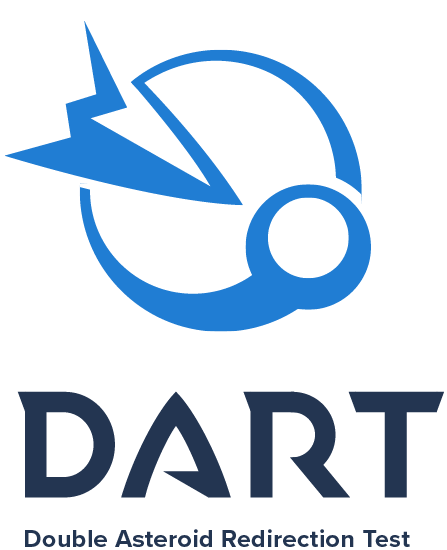
\includegraphics[scale=0.5]{figure/DART_mission_patch.png}
    \caption[Logo della missione DART.]{Logo della missione DART. (NASA/JHU-APL)}
    \label{fig:logo_DART}
\end{figure}

L'obiettivo principale della missione è quello di dimostrare l'efficacia dell'\textit{im}-\\
\textit{pattatore} \textit{cinetico} come metodo per la difesa planetaria dai PHA. Il target scelto per testare la tecnologia è il sistema binario di (65803) Didymos, in particolare la sua luna (65803) Didymos I Dimorphos (d'ora in avanti chiamata semplicemente Dimorphos). Il concetto alla base dell'impattatore cinetico è quello di colpire un asteroide con un oggetto massivo con una velocità sufficientemente alta da cambiare l'orbita del corpo \citep{rivkin_double_2021}.

\section{La difesa planetaria}
Come descritto nella \cref{sec:pha} la regione di spazio attorno alla Terra è densamente popolata di asteroidi potenzialmente pericolosi.\\
Negli anni è maturata sempre più la consapevolezza scientifica che questi oggetti rocciosi possono causare enormi danni al nostro pianeta in caso di collisione, ma al giorno d'oggi non esiste nessun sistema in funzione per la difesa planetaria.

Per questi motivi la comunità scientifica ha iniziato a teorizzare e progettare diversi sistemi anti-collisione con asteroidi (Asteroid Impact Avoidance, AIA), che comprendono tutti quei metodi con cui sarebbe teoricamente possibile deviare un asteroide in rotta di collisione con la Terra e che provocherebbe eventi distruttivi.\\
Un impatto da parte di un asteroide sufficientemente grande ($> 100\; m$), a seconda del luogo d'impatto, potrebbe causare massicci tsunami, tempeste di fuoco o un "inverno da impatto", dovuto al blocco della luce solare da parte di grandi quantità di polvere e altri detriti immessi nella stratosfera. Si ritiene che una collisione avvenuta 66 milioni di anni fa, tra la Terra e un oggetto di 10 chilometri di diametro, abbia generato il cratere di Chicxulub e abbia innescato l'estinzione del Cretaceo-Paleogene, che la comunità scientifica ritiene abbia portato all'estinzione di tutti i dinosauri non-aviani.\\
Più recentemente, gli eventi di Tunguska del 1908, quando una meteora di circa 65 metri esplose sopra i cieli della Siberia e devastò 2150 km$^2$ di foresta, o di Chelyabinsk del 2013, quando un oggetto di circa 20 metri esplose nei cieli russi causando danni a edifici e infrastrutture, hanno richiamato l'attenzione su tali minacce.

In letteratura sono stati descritti diversi metodi per la difesa planetaria. Tuttavia, nel marzo 2019, gli scienziati hanno riscontrato che gli asteroidi potrebbero essere molto più difficili da distruggere di quanto si pensasse in precedenza \citep{el_mir_new_2019}. In aggiunta, un asteroide può anche ricompattarsi grazie alla gravità, dopo essere stato distrutto. Nel marzo 2021, al termine della Planetary Defence Conference, gli astronomi e le astronome hanno dichiarato che, per evitare un impatto, potrebbero essere necessari dai 5 ai 10 anni di preparazione preliminare\footnote{\href{https://cneos.jpl.nasa.gov/pd/cs/pdc21/}{https://cneos.jpl.nasa.gov/pd/cs/pdc21/}}, per questo motivo è molto importante avere a disposizione dati orbitali molto precisi e una tecnologia di mitigazione pronta all'uso.

\subsection{Impattatore cinetico}
Le varie tecniche di prevenzione dalle collisioni presentano diversi compromessi rispetto a parametri quali le prestazioni complessive, i costi, i rischi di missione, le operazioni e le disponibilità tecnologiche \citep{canavan_interception_1992}. Esistono vari metodi per modificare l'orbita di un asteroide o di una cometa \citep{hall_ross_1997}, che possono essere catalogati in base al tipo di mitigazione (deflessione o frammentazione), la fonte di energia (cinetica, elettromagnetica, gravitazionale, solare/termica o nucleare) e la strategia di approccio (intercettazione o rendezvous \citep{solem_interception_1993}).

Dato l'argomento di questa tesi ci concentreremo sul metodo dell'impattatore cinetico.\\
Quando un asteroide è ancora lontano dalla Terra, un modo per deflettere la sua orbita è quello di alterare direttamente il suo momento facendo collidere una sonda sulla sua superficie. Analisi condotte da NASA nel 2007\footnote{\href{https://web.archive.org/web/20160305101217/http://neo.jpl.nasa.gov/neo/report2007.html}{https://web.archive.org/web/20160305101217/http://neo.jpl.nasa.gov/neo/report2007.html}} mostrarono che "gli impattatori cinetici non nucleari sono l'approccio più maturo e potrebbero essere usati in scenari di deflessione/mitigazione che coinvolgono piccoli oggetti singoli."

Il principio di deviazione, applicato poi dalla sonda DART, si basa sulla legge di conservazione del momento
\begin{equation}
    m_1 \vec{v}_1 + M_2\vec{v}_2 = (m_1+M_2)\vec{v}_3
\end{equation}
con $\vec{v}_1$ e $m_1$ velocità e massa della sonda, $\vec{v}_2$ e $M_2$ velocità e massa dell'asteroide e $\vec{v}_3$ velocità finale dopo l'impatto. 
La velocità della sonda rispetto al NEO è nell'ordine dei $10\,km/s$ e il momento è trasferito al NEO, causando un cambio nella sua velocità orbitale che risulta in una leggera deviazione dell'orbita.

\section{Double Asteroid Redirection Test}\label{sec:DART}
DART è una missione NASA che nasce con l'intento di dimostrare la fattibilità del metodo, sopradescritto, dell'impattatore cinetico.\\
NASA ed ESA hanno iniziato a collaborare nel 2015 al progetto AIDA\footnote{\href{https://www.esa.int/Space_Safety/Hera/Asteroid_Impact_Deflection_Assessment_AIDA_collaboration}{https://www.esa.int/Space\_Safety/Hera/Asteroid\_Impact\_Deflection\_Assessment\_AIDA\_collaboration}} (Asteroid Impact and Deflection Assessment), che consisteva in due sonde separate ma che avrebbero lavorato in sinergia \citep{michel_european_2018}. Inizialmente le due sonde avrebbero dovuto essere lanciate insieme, ma dopo varie modifiche al piano della missione la sonda ESA è stata differita e si è giunti alla configurazione finale: DART, gestita da NASA, e Hera, di cui parleremo in seguito, gestita da ESA.

Il 24 novembre 2021 la sonda DART è stata lanciata a bordo di un Falcon 9 verso la sua destinazione finale: il sistema di Didymos e Dimorphos.

\subsection{Strumentazione}
Poiché l'obiettivo della sonda era quello di collidere contro un asteroide, essa è stata dotata degli strumenti essenziali per la fase di crociera e di approccio, nonostante ciò aveva una massa di $610\,kg$.

\paragraph*{Camera}
Oltre ai sensori base per la navigazione nello spazio, la sonda ospitava una camera da $20\,cm$ di apertura chiamata DRACO (Didymos Reconnaissance and Asteroid Camera for Optical navigation). DRACO era basata sulla camera LORRI della sonda di NASA New Horizons e ha consentito la navigazione autonoma della sonda fino all'impatto al centro di Dimorphos.\\
La parte ottica della camera era costituita da un telescopio Ritchey-Chrétien equipaggiato con un teleobiettivo con campo di vista (FOV) di 0.29° e una lunghezza focale di $2.6208\,m$ (f/12.60). La risoluzione spaziale poco prima dell'impatto è stata di circa $20\,cm/px$.\\
Il sensore utilizzato era un CMOS con un range spettrale di $0.4-1\,\mu m$ (dal visibile al vicino infrarosso).

\begin{figure}
    \centering
    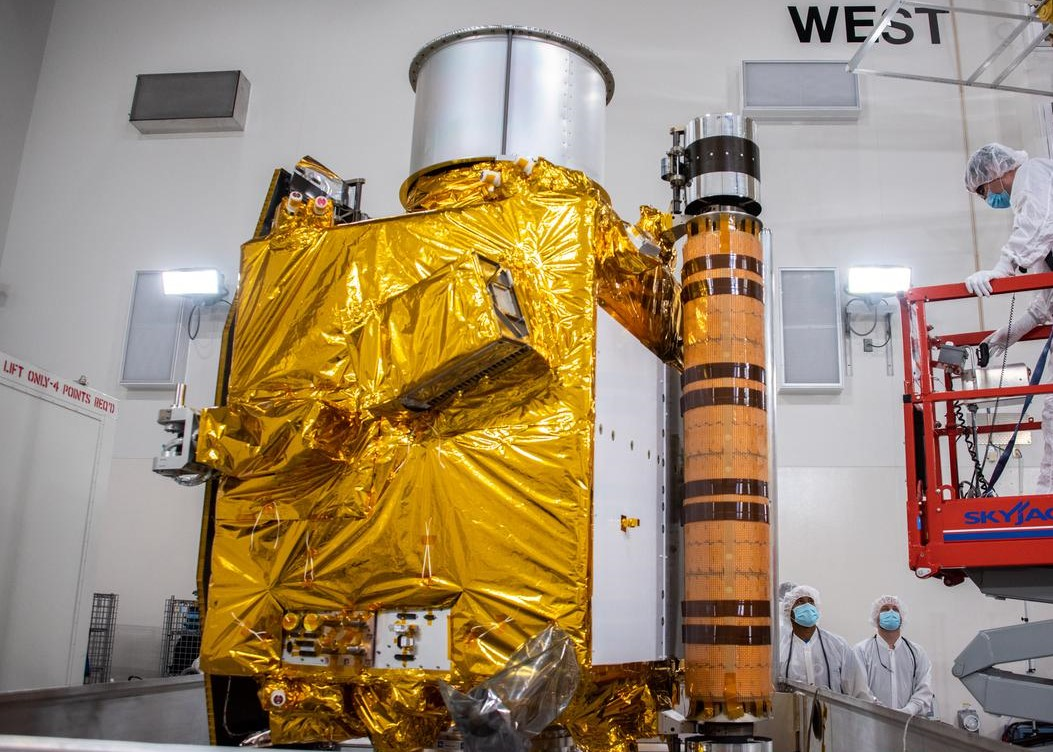
\includegraphics[scale=0.26]{figure/dart_cleanroom.jpg}
    \caption[La sonda DART nella clean room.]{La sonda DART appena installata sul payload adapter. Al centro è possibile vedere il dispenser di LICIACube. (NASA/JHU-APL)}
    \label{fig:dart_cleanroom}
\end{figure}

\paragraph*{LICIACube}
Per osservare l'impatto e l'evoluzione dei detriti (ejecta) da una distanza tale da poter avere un quadro generale del test, ASI e Argotec hanno progettato un cubesat da 6U ($10\,cm\times 20\,cm\times 30\,cm$), LICIACube (Light Italian CubeSat for Imaging of Asteroids), che si è separato da DART l'11 settembre 2022 e ha seguito tutta la missione da una distanza di sicurezza di $\sim 1250\,km$, effettuando un flyby di Dimorphos a $56.7\,km$ 2 minuti e 45 secondi dopo l'impatto della sonda con il satellite naturale.

A bordo di LICIACube ci sono due camere ottiche: LEIA (LICIACube Explorer Imaging for Asteroid) e LUKE (LICIACube Unit Key Explorer).

\qquad \small{\textbf{LEIA}} È una camera catadriottica monocromatica con un campo di vista molto stretto (2.06°) e una risoluzione al punto di minima distanza di $1.38\,m/px$.

\qquad \small{\textbf{LUKE}} Si tratta di una camera equipaggiata con un filtro RGB con pattern di Bayern, con un largo campo di vista (5°).\\
Durante il flyby LUKE ha osservato sia l'emisfero impattato che quello non impattato di Dimorphos con una risoluzione spaziale massima di $\sim 4.3\,m/px$. L'analisi spettrofotometrica dei dati ottenuti verrà usata per provare a indagare la composizione superficiale di Dimorphos. I dati spettrofotometrici permetteranno di indagare l'eterogeneità superficiale e mappare la composizione superficiale dell'oggetto, e anche di cercare materiali esogeni generati dalla collisione con altri asteroidi durante la storia evolutiva del sistema \citep{poggiali_expected_2022}. I risultati forniti da LUKE, insieme a quelli di LEIA e DRACO, permetteranno di investigare la geologia del sistema di Didymos-Dimorphos \citep{pajola_anticipated_2022}.

\subsection{Missione primaria}
Dopo 8 mesi di fase di crociera la camera DRACO è riuscita a rilevare Didymos a circa 32 milioni di km (\cref{fig:primo_contatto}) e DART ha così potuto iniziare a rifinire la sua traiettoria. 
L'11 settembre 2022, 15 giorni prima dell'impatto, LICIACube è stato rilasciato. 2 minuti e 30 secondi prima dell'impatto l'obiettivo si trovava a $920\,km$. La sonda DART ha impattato sulla luna Dimorphos il 27 settembre 2022 alle 01:14 ora italiana (\cref{fig:920_penultima_dart}).
L'impatto è avvenuto a $6.6\,km/s$, liberando circa 11 gigajoule di energia.
2 minuti e 45 secondi dopo l'impatto LICIACube ha effettuato il flyby di Dimorphos a $56.7\,km$.

\begin{figure}[!h]
\centering
	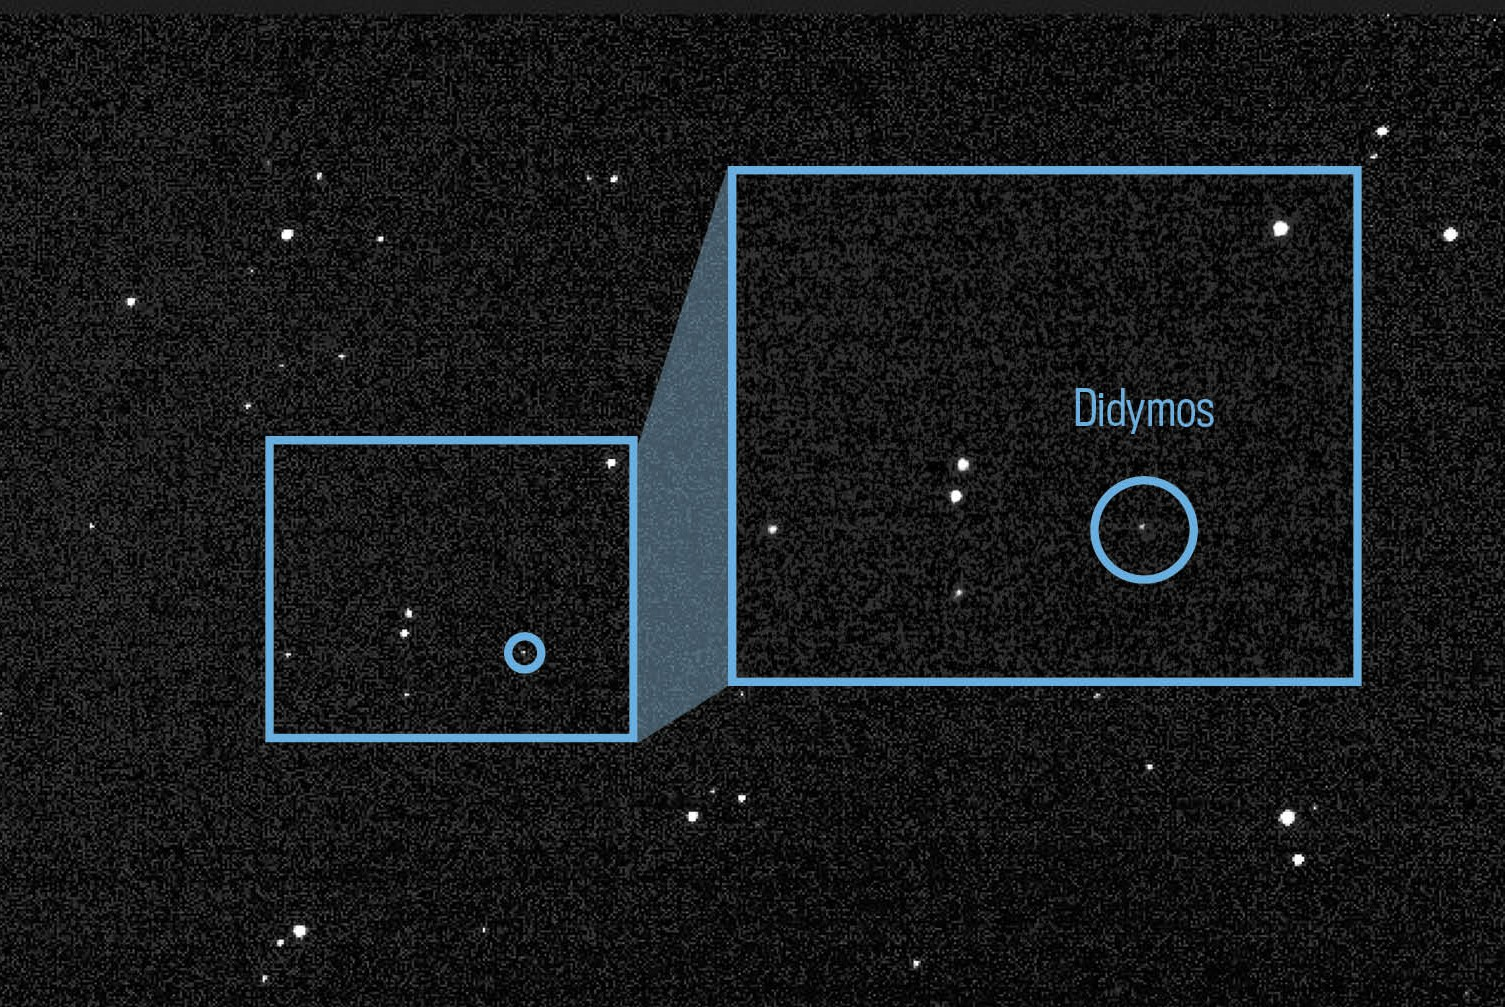
\includegraphics[width=.8\textwidth]{figure/primo_contatto.jpg}
\caption[Primo contatto della sonda DART con il sistema binario.]{Primo contatto della sonda DART con il sistema binario. (NASA/JHU-JPL)}
\label{fig:primo_contatto}
\end{figure}

\begin{figure}[!h]
\centering
	{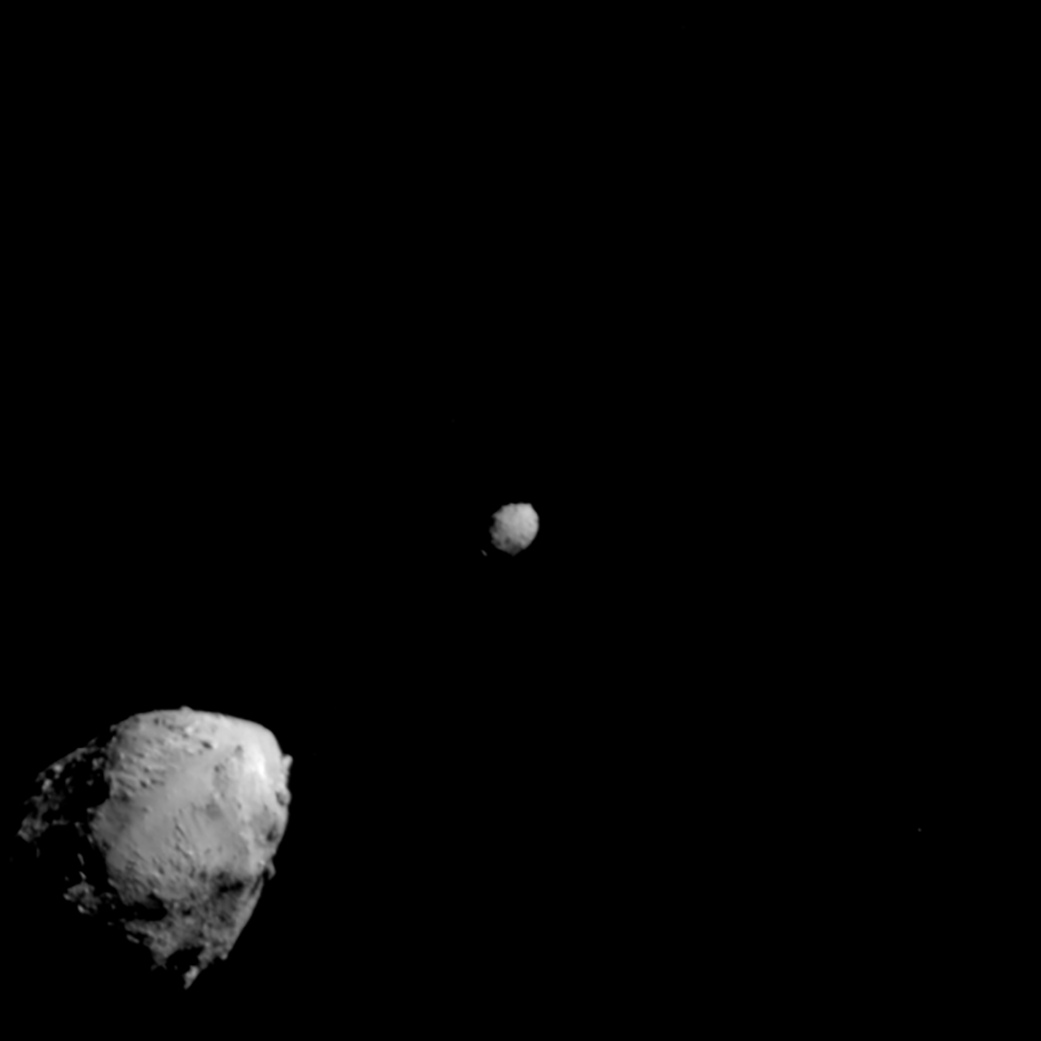
\includegraphics[width=.48\textwidth]{figure/920.png}} \quad
	{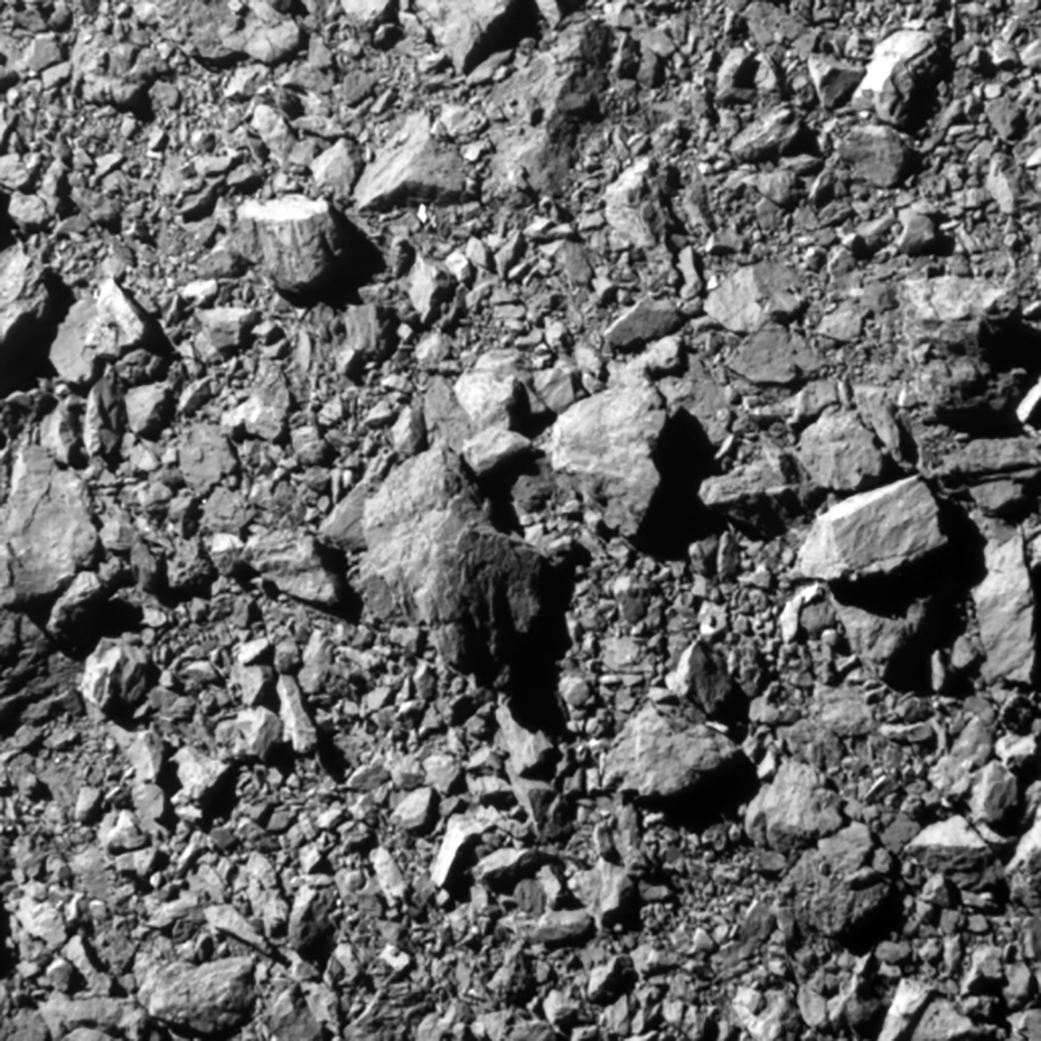
\includegraphics[width=.48\textwidth]{figure/penultima_dart.png}}
\caption[Immagini scattate dalla sonda DART in avvicinamento al sistema.]{Immagini scattate dalla sonda DART in avvicinamento al sistema. A sinistra il sistema binario visto da 920 metri di distanza, a destra la penultima immagine prima dell'impatto. (NASA/JHU-JPL)}
\label{fig:920_penultima_dart}
\end{figure}

\subsection{Campagna di osservazioni}
L'impatto è stato seguito da un gran numero di osservatòri terrestri e nello spazio (\cref{fig:obs_dart}).\\
Poiché la strumentazione a bordo della sonda era ridotta al minimo, la missione dipende quasi interamente dai dati raccolti dagli osservatòri nei giorni e mesi seguenti l'impatto.
Hubble Space Telescope (HST), James Webb Space Telescope (JWST), l'ATLAS Observatory e l'osservatorio SOAR hanno rilevato il pennacchio di ejecta qualche ora dopo l'impatto, misurandone l'estensione di più di $10000\,km$ (\cref{fig:hst_plume}). Sono state svolte osservazioni anche con il telescopio Copernico (e Galileo) dell'Osservatorio Astrofisico di Asiago e i dati raccolti saranno utilizzati per futuri lavori di analisi spettroscopica del sistema.\\
Nel \cref{ch:ch_5} verranno descritti i primi risultati ottenuti dopo l'impatto, le osservazioni svolte ad Asiago e le problematicità a esse connesse.

\begin{figure}[!h]
    \centering
    \includegraphics[scale=0.113]{figure/Telescopes_observing_DART's_impact.png}
    \caption[Osservatòri che hanno osservato l'impatto di DART.]{Lista di osservatòri che partecipano alla campagna si osservazioni post impatto. (NASA/JHU-APL)}
    \label{fig:obs_dart}
\end{figure}

\section{Missioni future}\label{sec:hera}
Come già anticipato nella \cref{sec:DART}, la missione DART verrà seguita dalla missione Hera\footnote{\href{https://www.heramission.space/}{https://www.heramission.space/}}, in sviluppo nei centri ESA, che dovrebbe essere lanciata nell'ottobre 2024 e dovrebbe arrivare in orbita attorno al sistema nel dicembre 2026.\\
L'obiettivo principale della missione sarà quello di valutare l'efficacia del metodo dell'impattatore cinetico sul sistema Didymos-Dimorphos. Per soddisfare questo obiettivo Hera dovrà determinare: 
\begin{itemize}
    \item quanto il trasferimento di momento dipende dalla densità, dalla porosità e dalla caratteristiche superficiali e interne dell'asteroide;
    \item in che percentuale l'energia cinetica è trasferita nella frammentazione e nella riorganizzazione dell'asteroide e quanta è trasformata in energia cinetica dei frammenti espulsi dall'impatto.
\end{itemize}

\begin{figure}[!h]
    \centering
    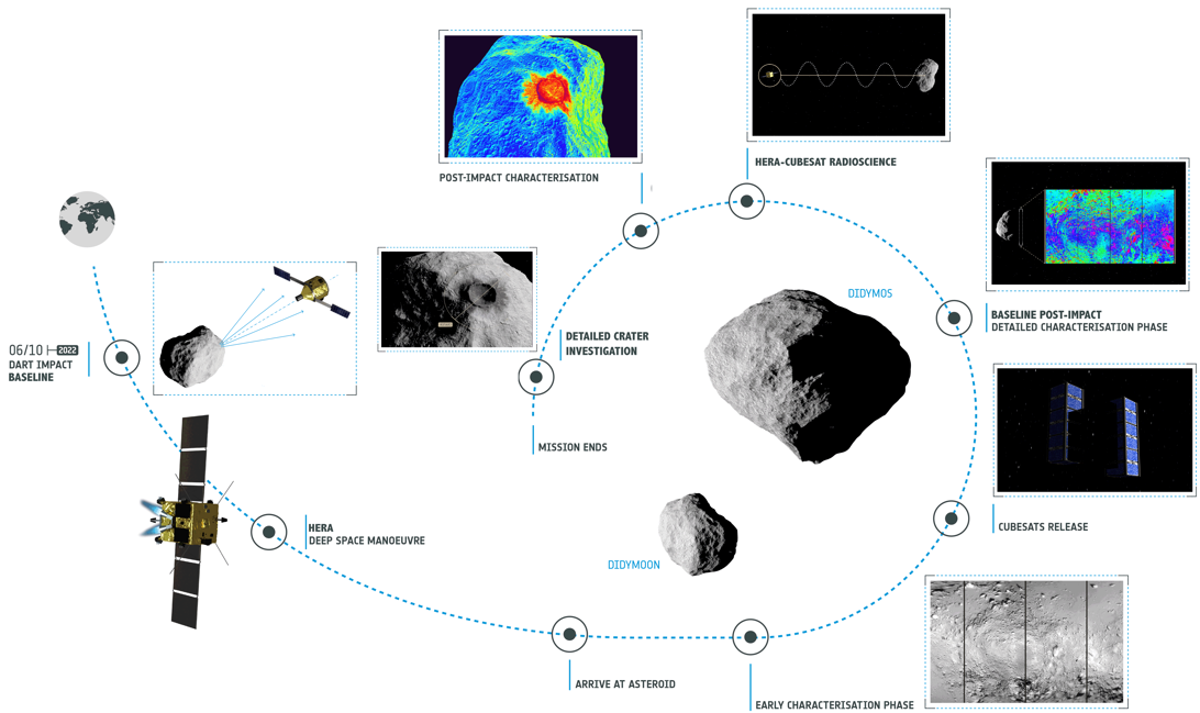
\includegraphics[scale=0.50]{figure/Hera_mission_timeline.png}
    \caption[Timeline della missione Hera.]{Timeline della missione Hera. (ESA)}
    \label{fig:hera_timeline}
\end{figure}

Hera ha anche altri obiettivi scientifici. Infatti, non dovendo impattare contro l'asteroide, sarà equipaggiata con vari strumenti scientifici:
\begin{itemize}
    \item \textbf{Hyperscout-H}: una camera iperspettrale per fornire immagini tra $665$ e $975\; nm$, in 25 diverse bande spettrali.
    \item \textbf{Planetary Altimeter (PALT)}: un micro-altimetro planetario con tecnologia LIDAR. L'accuratezza teorica di misurazione in altezza è di 0.5 metri.
    \item \textbf{Thermal Infrared Imager (TIRI)}: una camera termica a infrarossi fornita dall'Agenzia Spaziale Giapponese (JAXA). Il range spettrale è tra $7$ e $14\,\mu m$ ed è equipaggiata con 6 filtri. La risoluzione spaziale teorica è di 2.3 metri a 10 chilometri di altitudine.
    \item \textbf{X-Band Radio Science (X-DST)}: strumento radio che misurerà l'effetto Doppler dovuto ai disturbi radio e permetterà di ricavare la massa dei due asteroidi, le caratteristiche gravitazionali del sistema binario, le velocità orbitali e le orbite dei due corpi.
    \item Due cubesat: \textbf{Milani} e \textbf{Juventas} il cui scopo sarà quello di completare le informazioni scientifiche raccolte dalla sonda primaria.
\end{itemize}
Questi strumenti saranno necessari per raccogliere informazioni sui due asteroidi: caratteristiche superficiali, porosità e struttura interna. In particolare, Hera sarà la prima missione a mappare completamente la superficie e la struttura interna di un asteroide. L'intera luna Dimorphos verrà mappata globalmente con una risoluzione spettrale di qualche metro e il sito di impatto con una risoluzione prevista di 10 centimetri. Verrà inoltre studiato come si è evoluta la nube di frammenti generatasi dopo l'impatto e le caratteristiche dell'ambiente circostante i due corpi \citep{michel_esa_2022}.


\chapter{Il sistema di (65803) Didymos}\label{ch:ch_4}
Il sistema di (65803) Didymos è un sistema binario di Near Earth Asteroids.\\
Didymos (parola greca che significa "gemello", data la sua natura binaria), in origine chiamato 1996GT, è stato scoperto l'11 aprile 1996 dalla survey Spacewatch, eseguita dal Kitt Peak Observatory in Arizona. Durante il suo passaggio ravvicinato con la Terra nel novembre del 2003, è stato scoperto il suo satellite naturale Dimorphos (dal greco "che ha due forme", visto che la missione DART ne ha modificato l'aspetto). Le osservazioni pre-impatto, svolte negli anni passati, sono state eseguite dall'Ondrejov Observatory, dal Carbuncle Hill Observatory e dal Steward Observatory, per quanto riguarda la fotometria, mentre per quanto riguarda le osservazioni radar dall'osservatorio di Arecibo.\\
Successivamente, tra il 2003 e il 2022, sono state svolte altre osservazioni sia spettroscopiche che fotometriche che radar per poter caratterizzare al meglio il sistema in vista della missione DART, in particolare per stimare il suo periodo orbitale.

\section{Sistemi binari di asteroidi}\label{sec:binary_system}
Negli ultimi decenni il numero di NEA binari è più che quadruplicato e il numero di grandi MBA binari è duplicato. Le attuali evidenze osservative confermano che gli asteroidi binari piccoli ($\lesssim 20\,km$) si sono formati da eventi di fissione rotazionale e stabiliscono che l'effetto YORP è responsabile dell'aumento del tasso di rotazione. I grandi asteroidi ($\gtrsim20\,km$) con piccoli satelliti è più probabile che vengano creati durante grandi eventi collisionali.

\subsection{Introduzione}
I sistemi multipli di asteroidi sono importanti perché rappresentano una frazione considerevole della popolazione asteroidale e perché permettono di investigare molte proprietà, come le proprietà fisiche, la composizione, la struttura interna e i processi di formazione ed evoluzione, che sono spesso difficili da indagare con altri mezzi.\\
L'osservazione di sistemi multipli permette di derivare i valori di massa e densità di un gran numero di oggetti. Le misure di densità aiutano a comprendere la composizione e la struttura interna dei corpi minori. I sistemi binari offrono l'opportunità di misurare le proprietà termiche e meccaniche, che sono solitamente poco conosciute.

\subsection{Osservazioni}
\subsubsection{Osservazioni radar dei NEA binari}
Il radar si è rivelato un ottimo metodo per rilevare i secondari (la componente più piccola di un sistema binario) dei NEA. Nel complesso le osservazioni radar suggeriscono che circa un NEA, più grande di $200\,m$, su sei sia un sistema multiplo \citep{taylor_shape_2012}.\\
Le osservazioni nella regione radio possono essere usate per rilevare i satelliti di asteroidi grazie all'abilità di risolvere le componenti di un sistema sia spazialmente (lungo la linea di vista, LoS) che in termini di frequenza (spostamento Doppler della velocità rotazionale e di quella lungo la LoS), col risultato di ottenere una separazione tra le componenti misurabile in due dimensioni.\\
La maggior parte dei sistemi binari di NEA osservati fino a oggi consistono in un primario con una rotazione molto rapida e un secondario più piccolo, nell'ordine di 1/100 la dimensione del primario, la cui rotazione è sincronizzata al periodo orbitale mutuo. La maggioranza dei primari ruota in meno di 2.8 h.

\begin{figure}[!h]
    \centering
    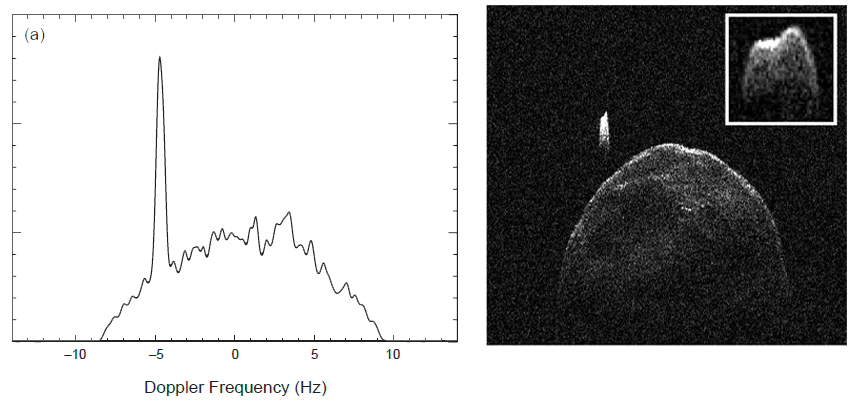
\includegraphics[scale=0.4]{figure/radar_image.png}
    \caption[Asteroide binario (285263) 1998 QE$_2$ rilevato dall'osservatorio di Arecibo.]{Asteroide binario (285263) 1998 QE$_2$ rilevato dall'osservatorio di Arecibo. \textbf{(a)} Potenza eco in funzione della frequenza Doppler. La banda radio molto stretta relativa al secondario (bloccato marealmente) spicca rispetto alla larga banda del primario. \textbf{(b)} Immagine radar. Le componenti sono risolte spazialmente (7.5 m/px). L'asse verticale rappresenta la distanza con l'osservatore, che aumenta verso il basso. L'asse orizzontale è la frequenza Doppler dovuta ai moti rotazionale e orbitale delle componenti. \citep{michel_asteroid_2015-1}}
    \label{fig:radar_image}
\end{figure}

Le forme e i volumi dei corpi, ottenuti dall'inversione delle immagini radar, combinate con la massa del sistema derivata dai moti orbitali, permettono di stimare la densità del sistema. Basse densità, nell'ordine di $1-2\;g/cm^3$ \citep{becker_physical_2015, brozovic_radar_2011}, suggeriscono una significativa macroporosità interna di almeno il 50\%, implicando una struttura rubble-pile (letteralmente \textit{agglomerato di detriti}). Con densità così basse, la rapida rotazione del primario può portare all'accumulo di materiale lungo la fascia equatoriale. La combinazione di rotazione rapida, forma, porosità e struttura rubble-pile hanno implicazioni sul meccanismo di formazione dei sistemi multipli di asteroidi.

\subsubsection{Osservazioni della curva di luce di NEA e MBA}
Una curva fotometrica consiste in una serie temporale di misurazioni della brillanza totale di un asteroide. La rilevazione di asteroidi binari tramite curva fotometrica si basa sul fatto che le componenti possono oscurare o proiettare un'ombra l'una sull'altra, producendo occultazioni o eclissi rispettivamente. Questo è il metodo principale utilizzato per lo studio del sistema di Didymos post impatto. Le tecniche di osservazione, analisi e modellazione sono state descritte da \citet{pravec_photometric_2006}, \citet{scheirich_modeling_2009}, \citet{scheirich_binary_2015}.

\begin{figure}[!h]
    \centering
    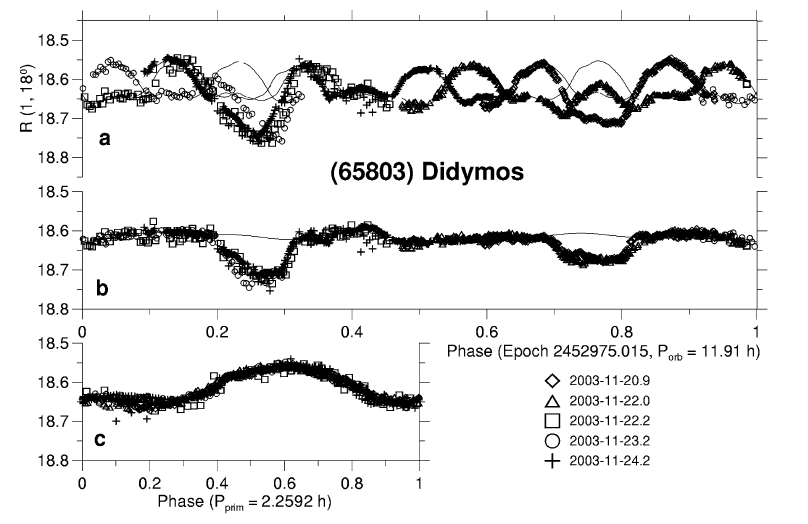
\includegraphics[scale=0.55]{figure/didymos_lightcurve.png}
    \caption[Curva di luce di (65803) Didymos.]{Curva di luce di Didymos ottenuta dai dati raccolti tra le notti del 20 e del 24 novembre 2003. \textbf{(a)} Curve di luce di entrambi le componenti. \textbf{(b)} Curva di luce della componente orbitale, derivata dopo la sottrazione della curva di luce del primario, che mostra l'evento di eclissi mutua tra le due componenti del sistema. \textbf{(c)} Curva di luce del primario. I dati sono stati confrontati con una serie di Fourier con parametri: priodo orbitale $P_{orb}=11.91$ h; periodo di rotazione del primario $P_{prim}=2.26$ h. \citep{pravec_photometric_2006}}
    \label{fig:didymos_lightcurve}
\end{figure}

Tra le scoperte principali ottenute con questo metodo c'è quella che stabilisce che gli asteroidi binari sono ubiqui. Sono stati trovati tra i NEA, tra i Mars Crossers e anche in tutta la Main Belt, sia all'interno di famiglie che non. C'è quindi il sospetto che i sistemi binari siano presenti tra i MBA tanto quanto lo sono tra i NEA.\\ Pare esserci un limite superiore al diametro del primario di circa $13\,km$ \citep{carry_small_2015}. Un limite inferiore non è ancora stato identificato univocamente.\\
Un'altra scoperta chiave è che i piccoli asteroidi binari hanno un momento angolare vicino al valore critico: questo valore è consistente con la formazione tramite fissione di un corpo progenitore con periodo di rotazione molto rapido e struttura rubble-pile poco coesa \citep{pravec_binary_2007}.\\
I poli orbitali degli asteroidi binari nella Main Belt mostrano una distribuzione altamente anisotropica, che si concentra entro 30° dai poli dell'eclittica \citep{pravec_binary_2012}. L'orientazione preferenziale dei poli suggerisce che i corpi progenitori fossero inclinati dall'effetto YORP verso stati di spin asintotici vicino a obliquità di 0 e 180 gradi.\\
Un'altra scoperta rilevante è che pare esserci un limite inferiore al valore della separazione tra le due componenti di un sistema binario $a/D_p=1.5$, corrispondente a un periodo orbitale di 11-12 h.\\

\subsubsection{Osservazioni spettrali di coppie di asteroidi}
Osservazioni di questo tipo possono essere intraprese quando il secondario ha una grande separazione angolare dal primario, quando il sistema è a eclissi/occultazione, o con l'aiuto di uno spettrografo a campo integrale.\\
Le osservazioni spettrali mostrano che le componenti di un sistema hanno spettri simili. In alcuni casi si è osservata una leggera discrepanza tra le componenti dovuta probabilmente alla differente quantità di SW.

\subsubsection{Imaging diretto di MBA binari}
L'imaging diretto di asteroidi può portare all'identificazione di uno o più satelliti e alla stima dei parametri orbitali. Questa modalità di osservazione rimane impegnativa perché i satelliti sono generalmente molto più piccoli e deboli rispetto ai primari e perché la maggior parte dei satelliti conosciuti orbita a distanze angolari sotto il secondo d'arco. La strumentazione in grado di ottenere i requisiti di contrasto e risoluzione include l'HST e i telescopi terrestri ($>10\,m$) equipaggiati con ottica adattiva.

\begin{figure}[!h]
    \centering
    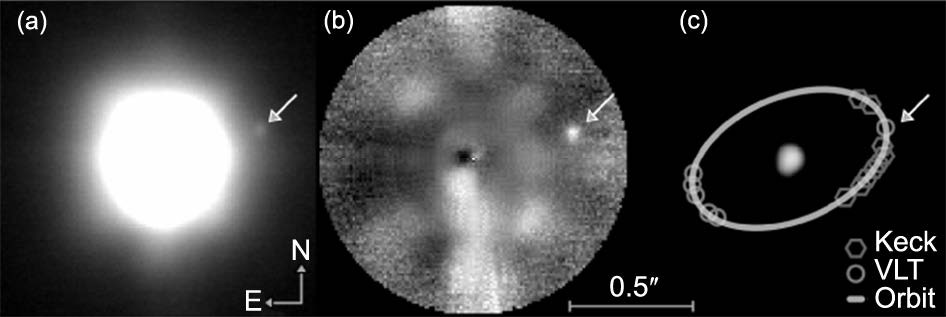
\includegraphics[width=0.9\textwidth]{figure/binaries_direct_imaging.jpg}
    \caption[Rilevazione del satellite di (41) Daphne grazie all'uso dell'ottica adattiva.]{Rilevazione di un satellite grazie all'utilizzo di ottica adattiva. \textbf{(a)} Immagine di (41) Daphne ottenuta con la camera NACO al VLT (5 s di esposizione). \textbf{(b)} Stessa immagine ma a cui è stato sottratto il flusso del primario, permettendo una misura più accurata del flusso e della posizione del secondario. \textbf{(c)} Determinazione dell'orbita. \citep{carry_ao_2009}}
    \label{fig:binaries_direct_imaging}
\end{figure}

La frazione di grandi MBA con satelliti è difficile da stimare data la complessa dipendenza dell'osservabilità del satellite dalla separazione angolare e dal rapporto di flussi tra primario e secondario. I satelliti conosciuti hanno un rapporto tra le masse con il primario tra $10^{-6}$ e $10^{-2}$. Tutti hanno un periodo orbitale tra 1 e 5.5 giorni. Molte orbite hanno eccentricità vicine a zero, valori dovuti a effetti di smorzamento tramite forze mareali.

\subsection{Formazione dei sistemi di piccoli asteroidi}
Si è visto come gli asteroidi primari di piccoli sistemi binari abbiano rotazioni molto rapide. Inoltre quasi tutti i piccoli asteroidi binari conosciuti hanno un elevato momento angolare. Queste caratteristiche non sono consistenti con una formazione in seguito a un evento sub-catastrofico, a una cattura tramite interazione a tre corpi o a una cattura dopo un impatto catastrofico. Sono invece indice di una formazione tramite fissione rotazionale. La fissione rotazionale prevede che un corpo progenitore possa essere messo in una rotazione così rapida che le forze centrifughe sovrastano quella gravitazionale, che mantiene coeso l'asteroide.

\citet{jacobson_dynamics_2011} hanno mostrato che dopo la fissione rotazionale ci sono varie possibili alternative all'evoluzione del sistema. Le loro simulazioni numeriche hanno portato alla stesura del diagramma mostrato in \cref{fig:binaries_evolution}. La distinzione tra alto e basso rapporto di massa $q$ gioca un ruolo importante nel distinguere due percorsi evolutivi. Lungo $q\gtrsim0.2$, entrambi i corpi si sincronizzano tramite forze mareali ed evolvono poi in base all'effetto Binary-YORP.\\
Lungo $q\lesssim0.2$ il sistema binario è non-legato. Durante la fase caotica il sistema può andare incontro a un altro episodio di fissione rotazionale. La materia persa da un corpo può accrescere il primario, contribuendo alla formazione del crinale equatoriale (una descrizione della formazione del possibile crinale equatoriale di Didymos è fornita nella \cref{sec:eq_ridge}), o può fuggire dal sistema. Se avviene quest'ultimo evento ci sono tre possibili risultati: si forma un asteroide con una forma diversa, una coppia di asteroidi o un sistema binario stabile. Successivamente, in quest'ultimo caso il secondario si sincronizza con il primario a causa delle forze mareali. In seguito il sistema evolve in base a come agiscono l'effetto BYORP e le forze mareali.

\begin{figure}[!h]
    \centering
    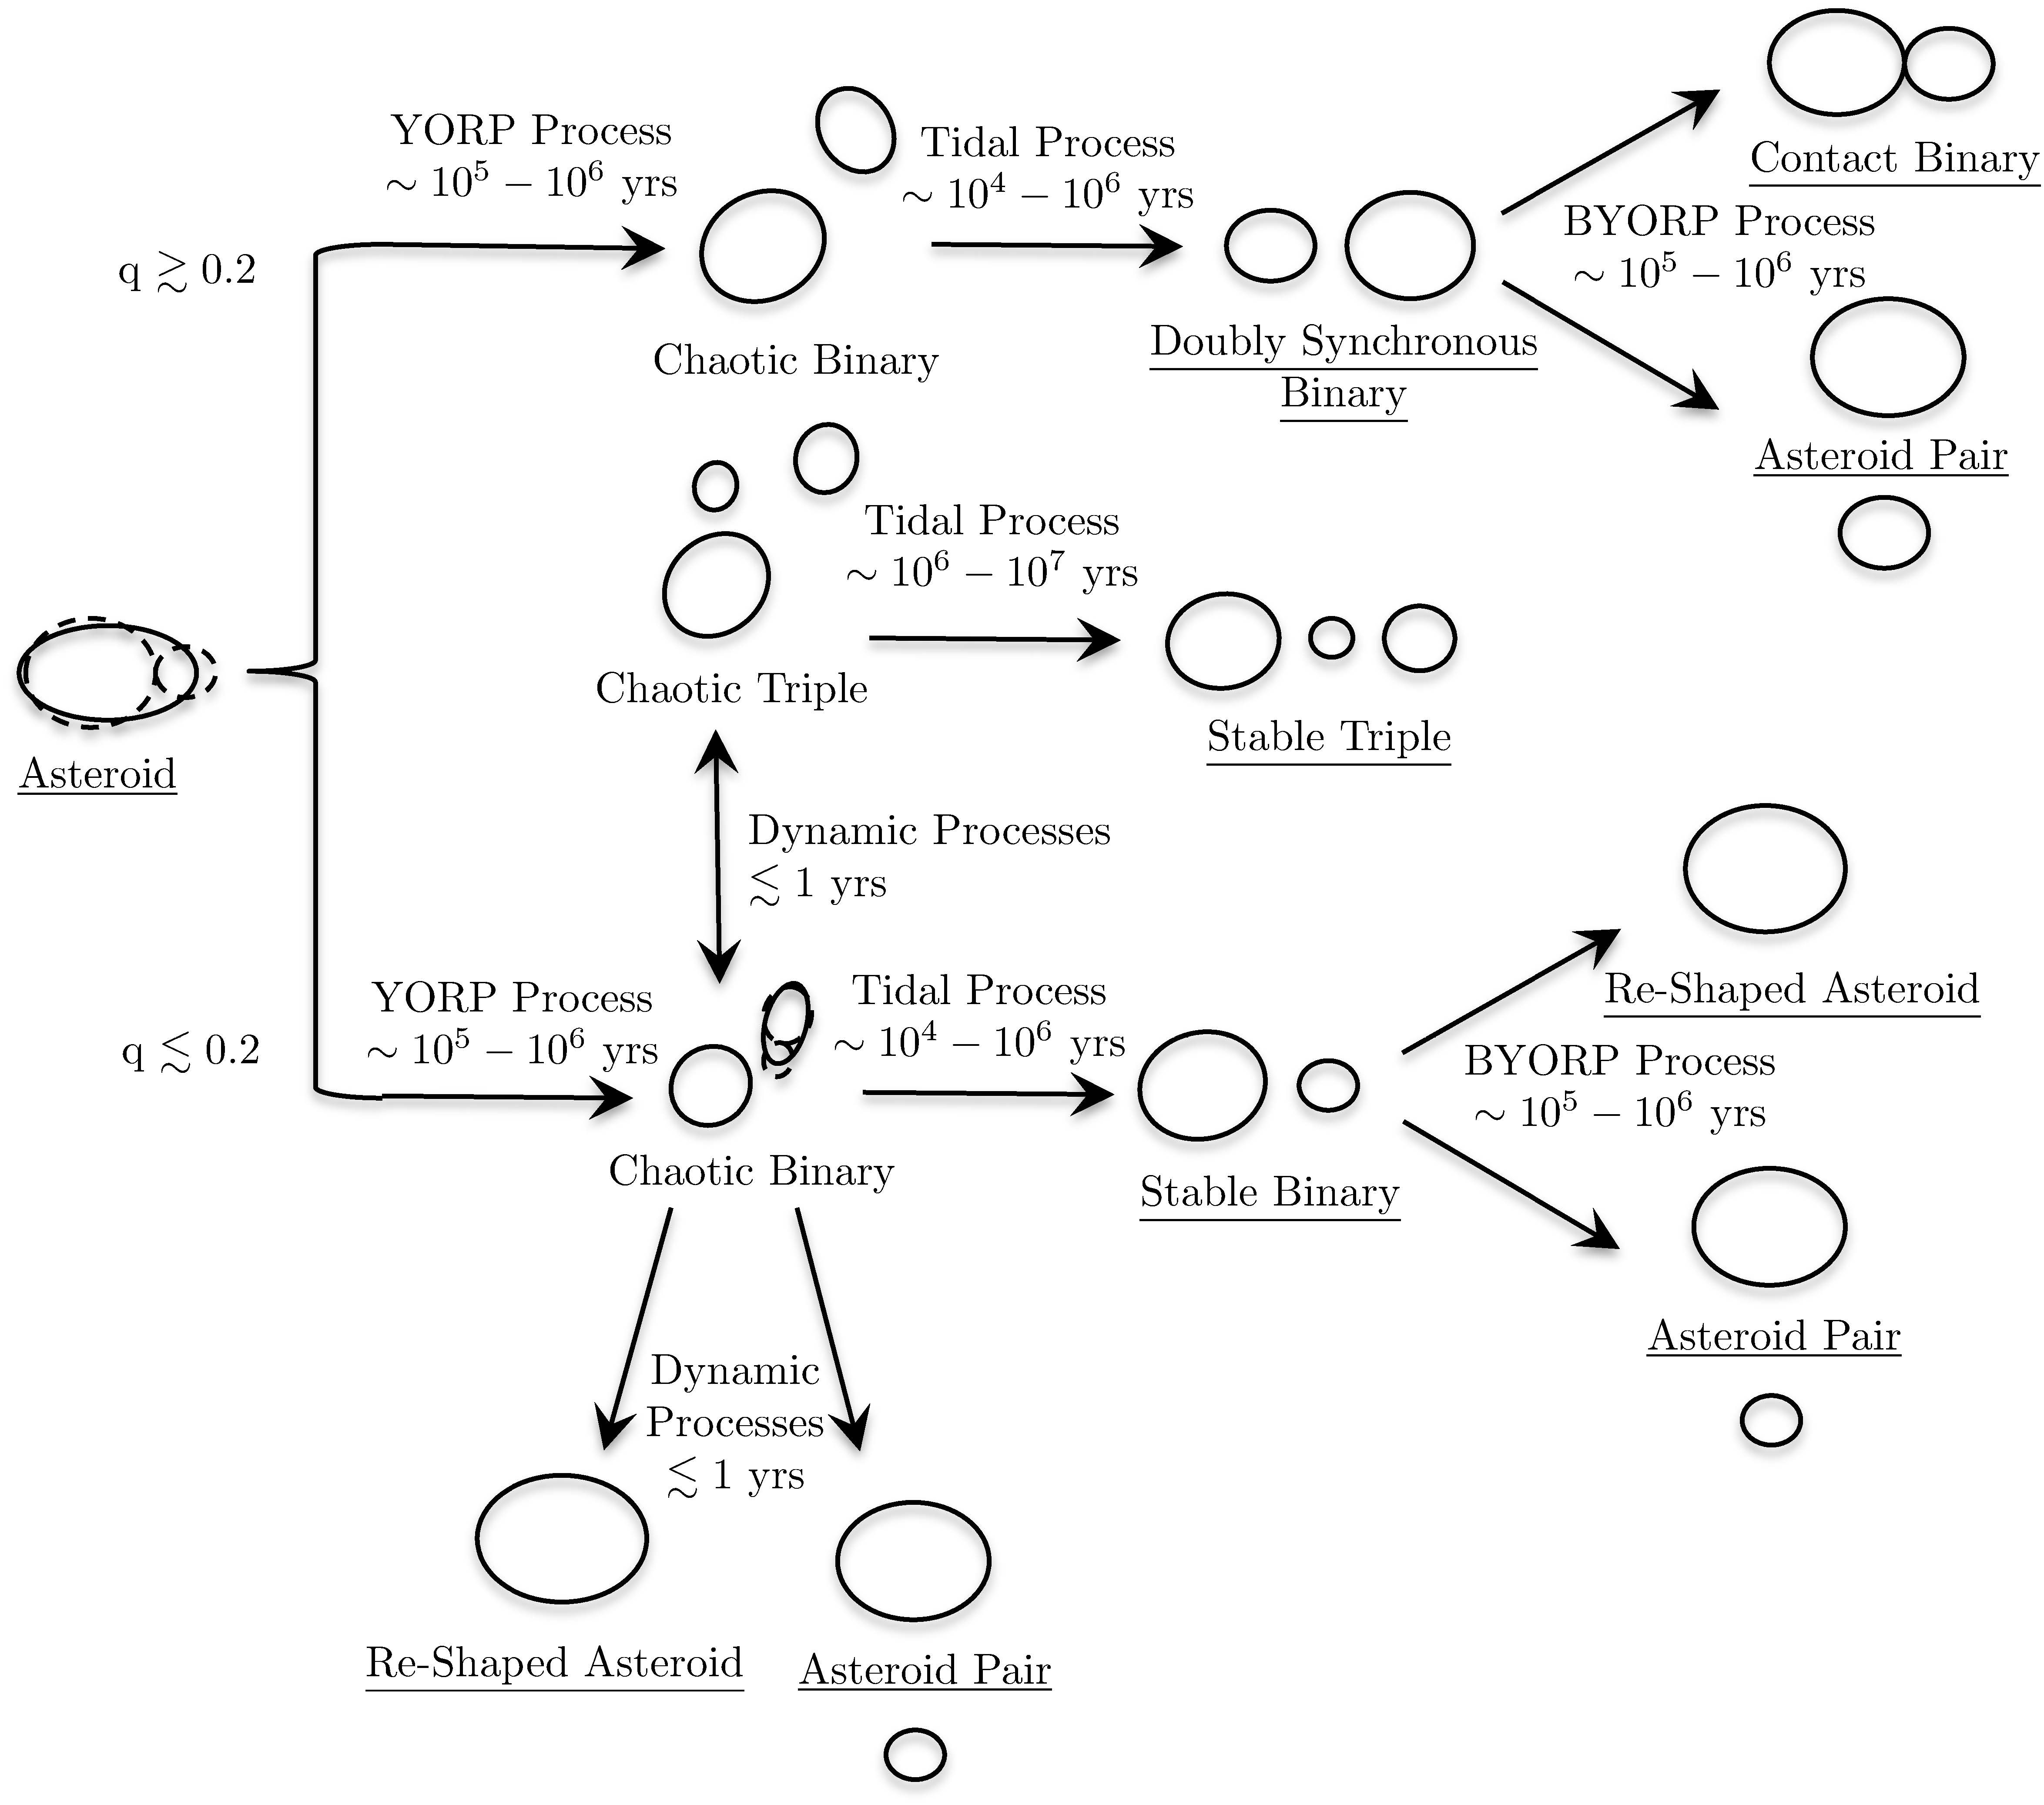
\includegraphics[scale=0.65]{figure/binaries_evolution.jpg}
    \caption[Diagramma dei possibili percorsi evolutivi di un piccolo asteroide.]{Diagramma dei possibili percorsi evolutivi di un asteroide dopo la fissione rotazionale. Le fasi sottolineate sono stabili in un tempo scala dell'effetto YORP. $q$ è il rapporto tra la massa del secondario e del primario. \citep{jacobson_dynamics_2011}}
    \label{fig:binaries_evolution}
\end{figure}

\section{Caratteristiche dinamiche}
Il sistema di Didymos, con un afelio di 2.2753 AU e un perielio di 1.0131 AU, fa parte della famiglia Apollo\footnote{Il suo perielio è minore di 1.017 AU, afelio dell'orbita terrestre (\cref{tab:asteroid-classification}).} (\cref{fig:orbit_view}).

\begin{figure}[!h]
    \centering
    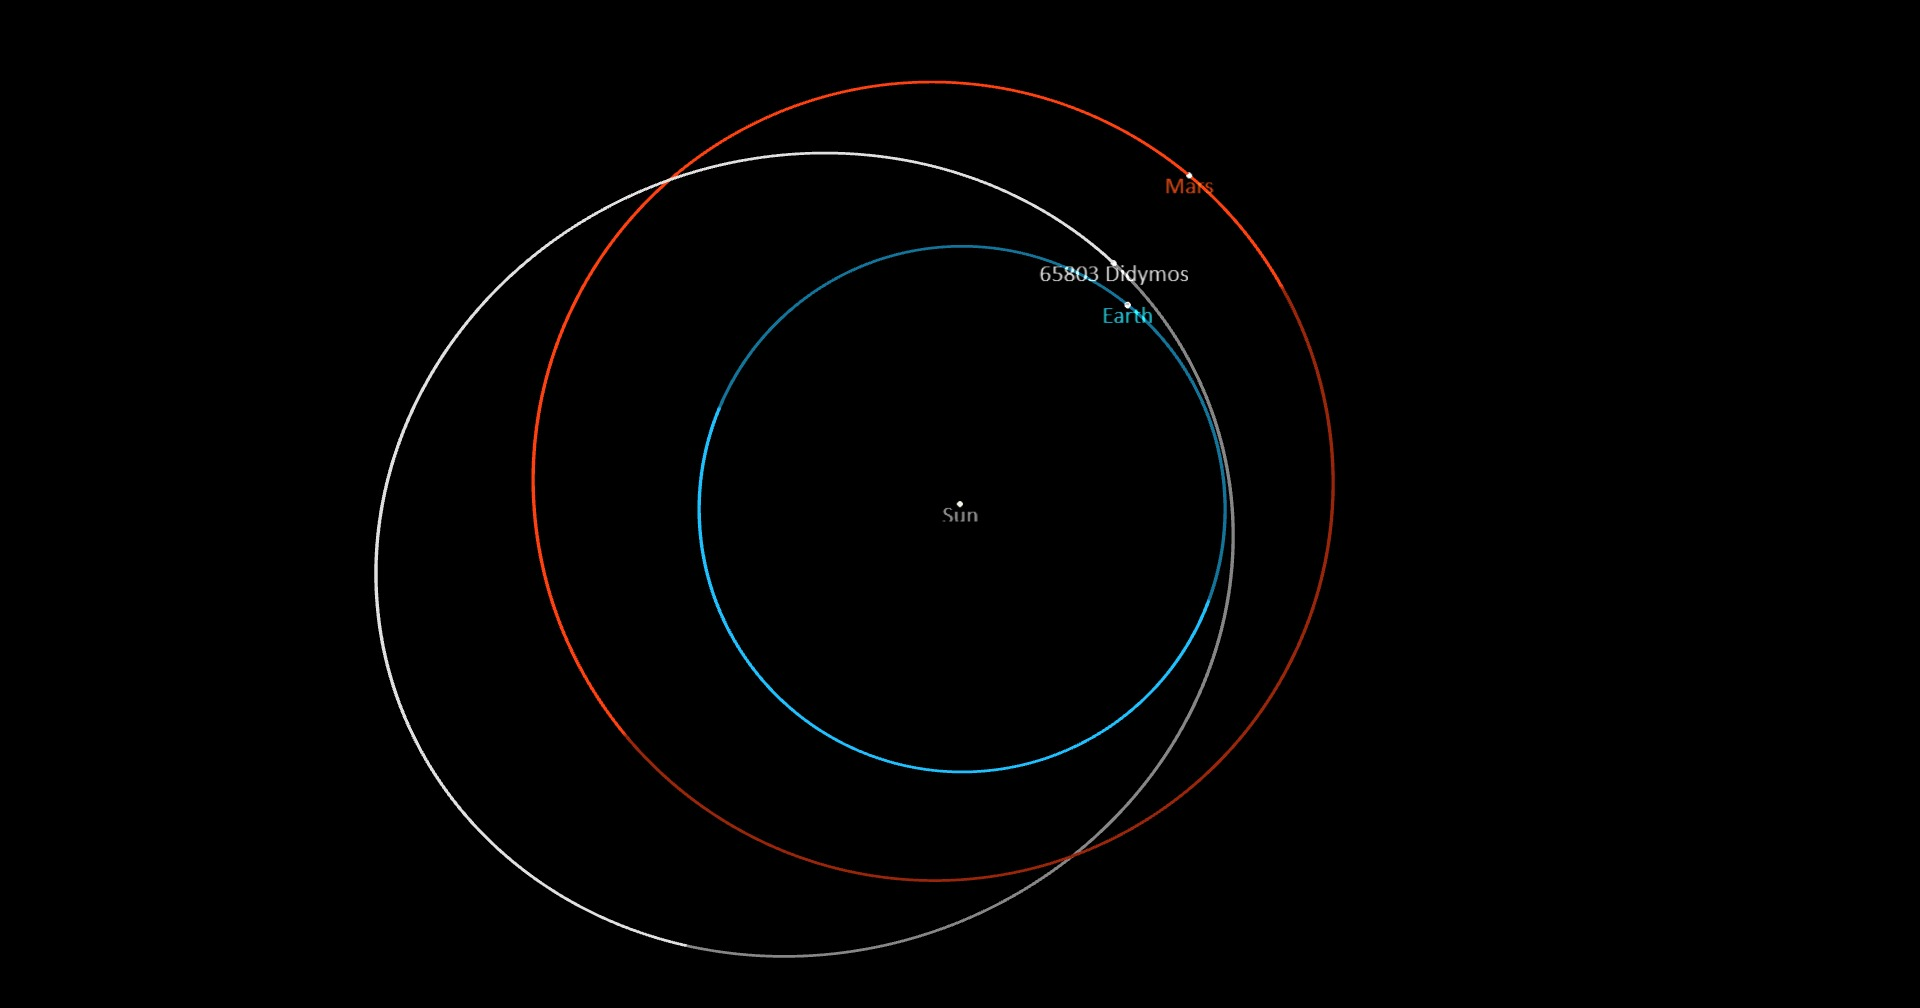
\includegraphics[scale=0.18]{figure/orbit_viewer.jpg}
    \caption[Vista dell'orbita di (65803) Didymos.]{Vista dell'orbita di (65803) Didymos, in bianco, confrontata con quella di Terra e Marte, rispettivamente in blu e rosso. (NASA/JPL)}
    \label{fig:orbit_view}
\end{figure}

Confrontando i dati radio raccolti nel 2003 e rianalizzati da \citet{naidu_radar_2020}, la larghezza di banda del secondario suggerisce un periodo di rotazione di $12.4\pm 3.0$ h, valore consistente con una rotazione che è sincronizzata con il periodo orbitale mutuo di 11.9 h. Usando il delay nel segnale e le separazioni Doppler si è ottenuto un valore del semiasse maggiore del sistema di $1190\pm 30\, m$, un'eccentricità $\leq 0.03$ e un periodo orbitale di $11.93\pm 0.01$ h\footnote{Un riassunto dei parametri è consultabile nella \cref{tab:param_didymos}.}, valori consistenti con i precedenti lavori di \citet{scheirich_modeling_2009} e \citet{fang_near-earth_2012} (\cref{fig:system_orbit}).\\
L'analisi delle proprietà rotazionali del sistema è importate per lo studio delle proprietà dinamiche poiché Didymos appartiene a una classe di asteroidi binari il cui primario è a rischio di distruzione rotazionale \citep{walsh_rotational_2008}.\\
Riguardo la sua origine dinamica nella Main Belt, \citet{richardson_dynamical_2016} ha suggerito che Didymos abbia raggiunto la sua orbita attuale molto probabilmente ($>$82\%) uscendo dalla Main Belt interna, vicino o all'interno della risonanza $\nu_6$, situata tra 2.1 e 2.5 AU.

\begin{figure}[!h]
    \centering
    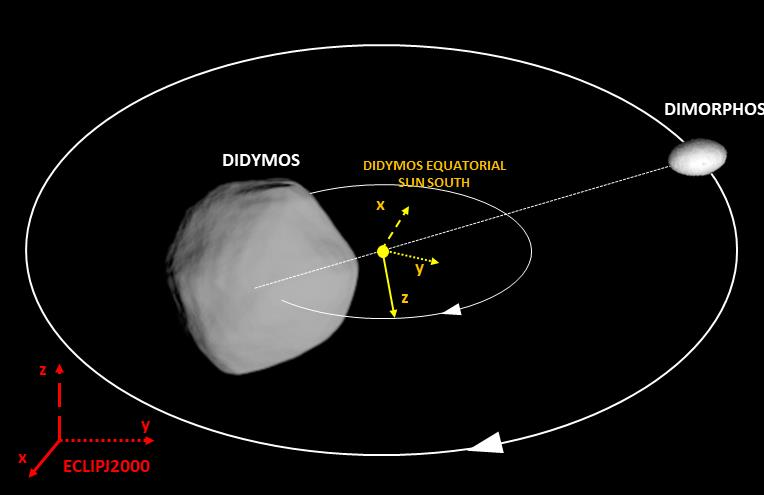
\includegraphics[scale=0.78]{figure/system_orbit.jpg}
    \caption[Geometria del sistema di Didymos.]{Geometria del sistema di Didymos. In giallo e arancio sono evidenziati i sistemi di riferimento. \citep{bottiglieri_applied_2022}}
    \label{fig:system_orbit}
\end{figure}

\subsection{Deriva dell'orbita del sistema}
Il valore osservato della deriva quadratica (\textit{quadratic drift}) nell'anomalia media è $\Delta M_d=0.15\pm 0.14\; deg\,yr^{-2}$. Esprimendo $\Delta M_d$ in termini del semiasse maggiore dell'orbita mutua $a$, $\Delta M_d=-\frac{3n\dot{a}}{4a}$, la deriva dell'anomalia media implica uno spostamento verso valori minori del semiasse maggiore con un tasso \\$\dot{a}=-0.09 \pm 0.08\;cm\,yr^{-1}$ \citep{scheirich_preimpact_2022}. 

Due sono i possibili meccanismi in grado di spiegare questa deriva:

\qquad \textit{(a)} L'effetto YORP binario (BYORP) è un cambio secolare dell'orbita reciproca di un sistema binario di asteroidi con un satellite sincrono dovuto all'emissione di radiazione termica dalla forma asimmetrica di quel satellite. \citet{pravec_binary_2010} hanno previsto che il valore della deriva quadratica di Didymos dovuta all'effetto BYORP sarebbe dovuta essere pari a $2.51\;deg\,yr^{-1}$, valore molto superiore al valore stimato da \citet{scheirich_preimpact_2022}. Più recentemente, \citet{jacobson_dynamics_2011} hanno presentato una teoria migliorata che incorpora sia l'effetto BYORP che le forze mareali tra le due componenti. Hanno mostrato che potrebbe esistere un equilibrio stabile a lungo termine tra queste due forze, nel caso in cui l'effetto BYORP sottragga momento angolare all'orbita. Poiché il periodo di rotazione di Didymos è minore del periodo orbitale di Dimorphos, il satellite crea un rigonfiamento mareale sul primario che sottrae energia alla rotazione del primario e la trasferisce al momento angolare orbitale. Queste forze fanno evolvere l'orbita reciproca fino a un valore del semiasse maggiore in cui essa è in equilibrio e quindi non evolve ulteriormente. Il valore riscontrato della deriva dell'anomalia media potrebbe indicare che il sistema stia evolvendo, e sia molto vicino, a questo equilibrio.

\qquad \textit{(b)} L'effetto Yarkovsky non solo influenza il moto del centro di massa del sistema binario ma anche il moto relativo delle due componenti. Per NEA binari la deriva del semiasse maggiore è nell'ordine di $\sim 1$ - qualche $mm\,yr^{-1}$ \citep{scheirich_satellite_2021}, stesso ordine di grandezza del $\Delta M_d$ osservato per Didymos.

\section{Caratteristiche fisiche e morfologiche}
\citet{naidu_radar_2020}, analizzando i dati radar raccolti con il radiotelescopio di Arecibo nel 2003 e includendo le curve di luce ottenuta da \citet{pravec_photometric_2006}, ha ottenuto una stima del modello della forma del sistema di Didymos. Il primario, in base a questo modello, risultava a forma "top-shaped" (letteralmente \textit{a forma di trottola}) con un rigonfiamento equatoriale. Il diametro equivalente risulterebbe di $780\pm 30\,m$ e le estensioni lungo i tre assi principali sarebbero $832\,m$, $838\,m$, $786\,m$ (con un'incertezza del 6\% sugli assi x e y, e del 10\% sull'asse z). Il valore calcolato per la densità risulta essere di $2.17\pm 0.35\;g\,cm^{-3}$. I dati radar non contengono una rotazione completa del secondario, Dimorphos, ma mostrano un'estensione visibile di circa $75\,m$, implicando un diametro di $150\pm 30\,m$. Osservazioni recenti hanno stimato un diametro equivalente di $171\pm 11\; m$ \citep{scheirich_preimpact_2022}\footnote{Un riassunto dei parametri è consultabile nella \cref{tab:param_didymos}.}.


\subsection{Modellizzazione della forma}\label{sec:shape_model}

\begin{figure}[!h]
    \centering
    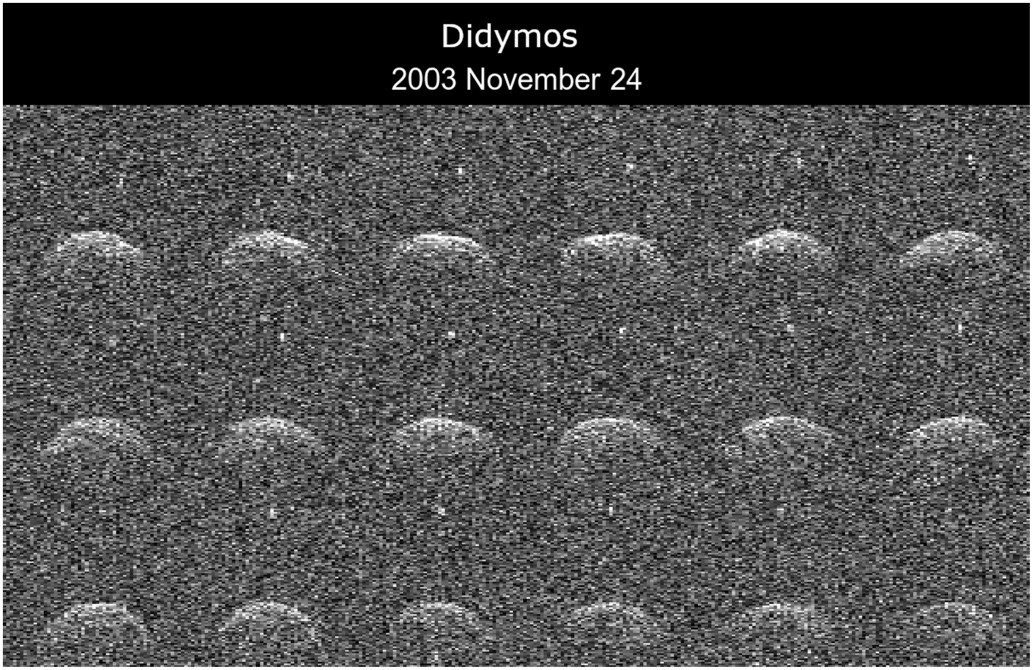
\includegraphics[scale=1.3]{figure/didymos_241103.jpg}
    \caption[Immagini delay-Doppler ottenute con il telescopio di Arecibo.]{Immagini delay-Doppler ottenute con il telescopio di Arecibo il 24 novembre 2003 tra le 03:15 e le 05:09 UTC. Ogni immagine è la somma di tre pose, durante le quali il primario ha ruotato di 14°. La risoluzione dell'immagine è di $0.1\,\mu s\times 0.3\,Hz$. \citep{naidu_radar_2020}}
    \label{fig:didymos_241103}
\end{figure}

La \cref{fig:didymos_shape_model} mostra la vista dei principali assi del modello di "best-fit" finale basato sui dati sopra descritti. Una delle caratteristiche più prominenti, nel modello, è una faccia\footnote{Superficie piatta su una figura geometrica.} sul rigonfiamento equatoriale lunga $\sim 350\,m$. Un'altra piccola faccia è presente a circa 120° in longitudine dalla prima. Il resto della superficie appare regolare su scale inferiori a $100\,m$, ma è un fattore probabilmente dovuto alla mancanza di caratteristiche nei dati dovuta al basso rapporto segnale-rumore ($S/N$) e alla bassa risoluzione, e non implica che la superficie sia effettivamente regolare su scale decametriche.\\
La maggior parte dei punti delle curve di luce corrispondono in modo ottimale al modello della forma, ma ci sono delle eccezioni. Queste potrebbero essere dovute a diversi fattori quali una topografia su scala minore che non è visibile nelle immagini radar, uno scattering ottico non ottimale sulla superficie e le assunzioni fatte nel definire i modelli di scattering ottico e radar.

\begin{figure}
    \centering
    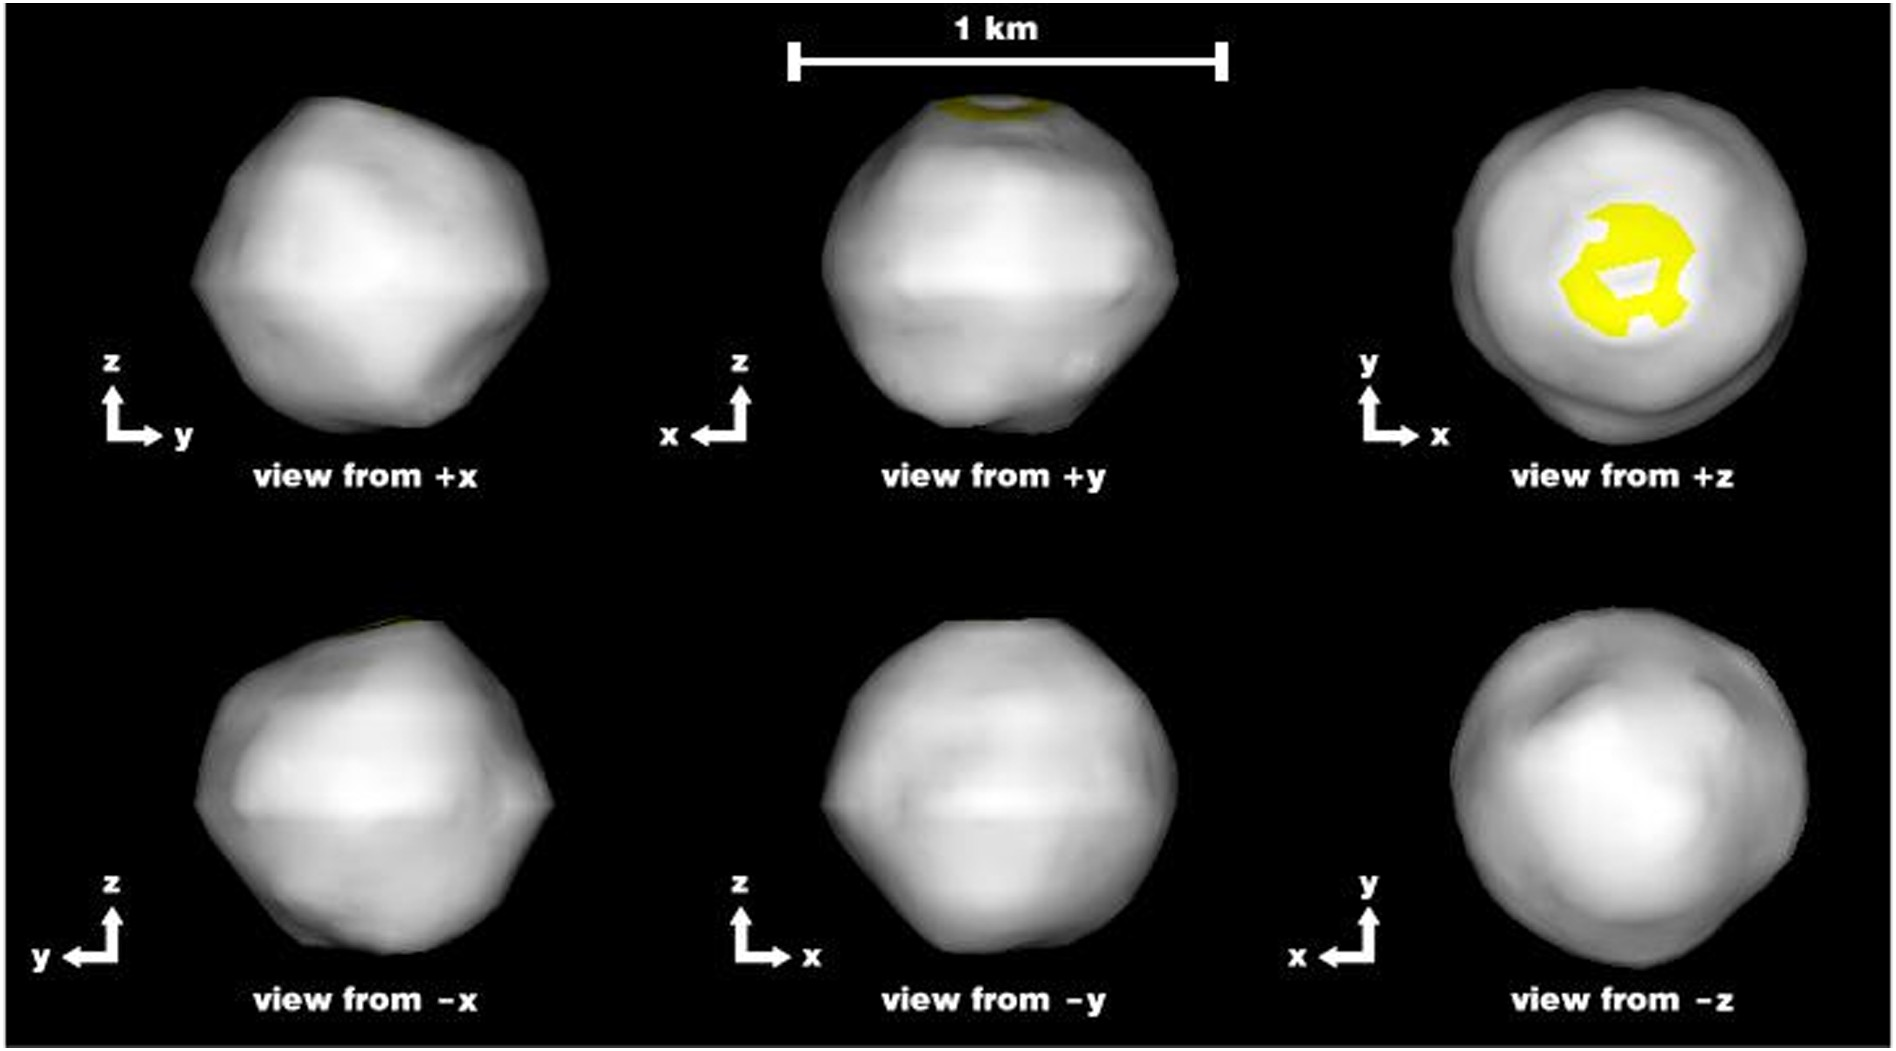
\includegraphics[scale=0.78]{figure/didymos_shape_model.jpg}
    \caption[Vista degli assi principali del modello della forma del primario.]{Vista degli assi principali del modello della forma del primario. Il modello ha 1000 vertici e 1996 facets triangolari. La risoluzione efficace è $\sim 50\,m$. Le regioni in giallo indicano regioni in cui l'angolo di incidenza e di scattering è $>60^\circ$. \citep{naidu_radar_2020}}
    \label{fig:didymos_shape_model}
\end{figure}

\subsection{Formazione del crinale equatoriale}\label{sec:eq_ridge}

Per lo studio della formazione del rigonfiamento equatoriale sono stati presi in considerazione due modelli con tassi di rotazione diversi (\cref{fig:failure_models}): uno con il periodo di rotazione attuale di 2.26 h, l'altro con un periodo più lungo, di 3.5 h, che è il caso in cui si trovava Didymos nel passato.\\
Nel caso del periodo di 2.26 h si ottiene che l'asteroide debba essere andato incontro a un cedimento strutturale interno. Questo ha comportato una deformazione verso l'esterno del piano equatoriale e una deformazione verticale in altre regioni, modalità di cedimento consistente con altri asteroidi top-shaped con rotazioni rapide \citep{hirabayashi_rotationally_2019}.\\
Diversamente, il caso del periodo di rotazione di 3.5 h mostra una modalità di cedimento differente. \citet{hirabayashi_failure_2015} ha previsto che se un oggetto sferoidale che ruota lentamente ha una coesione vicino a zero, allora le condizioni superficiali diventano più sensibili al cedimento rispetto a quelle interne. Il modello mostra, quindi, zone di cedimento locale sparse per tutta la superficie ma che tendono a collocarsi a basse latitudini, dove la pendenza del campo gravitazionale è ripida. I vettori di deformazione puntano principalmente verso l'interno.

\begin{figure}
    \centering
    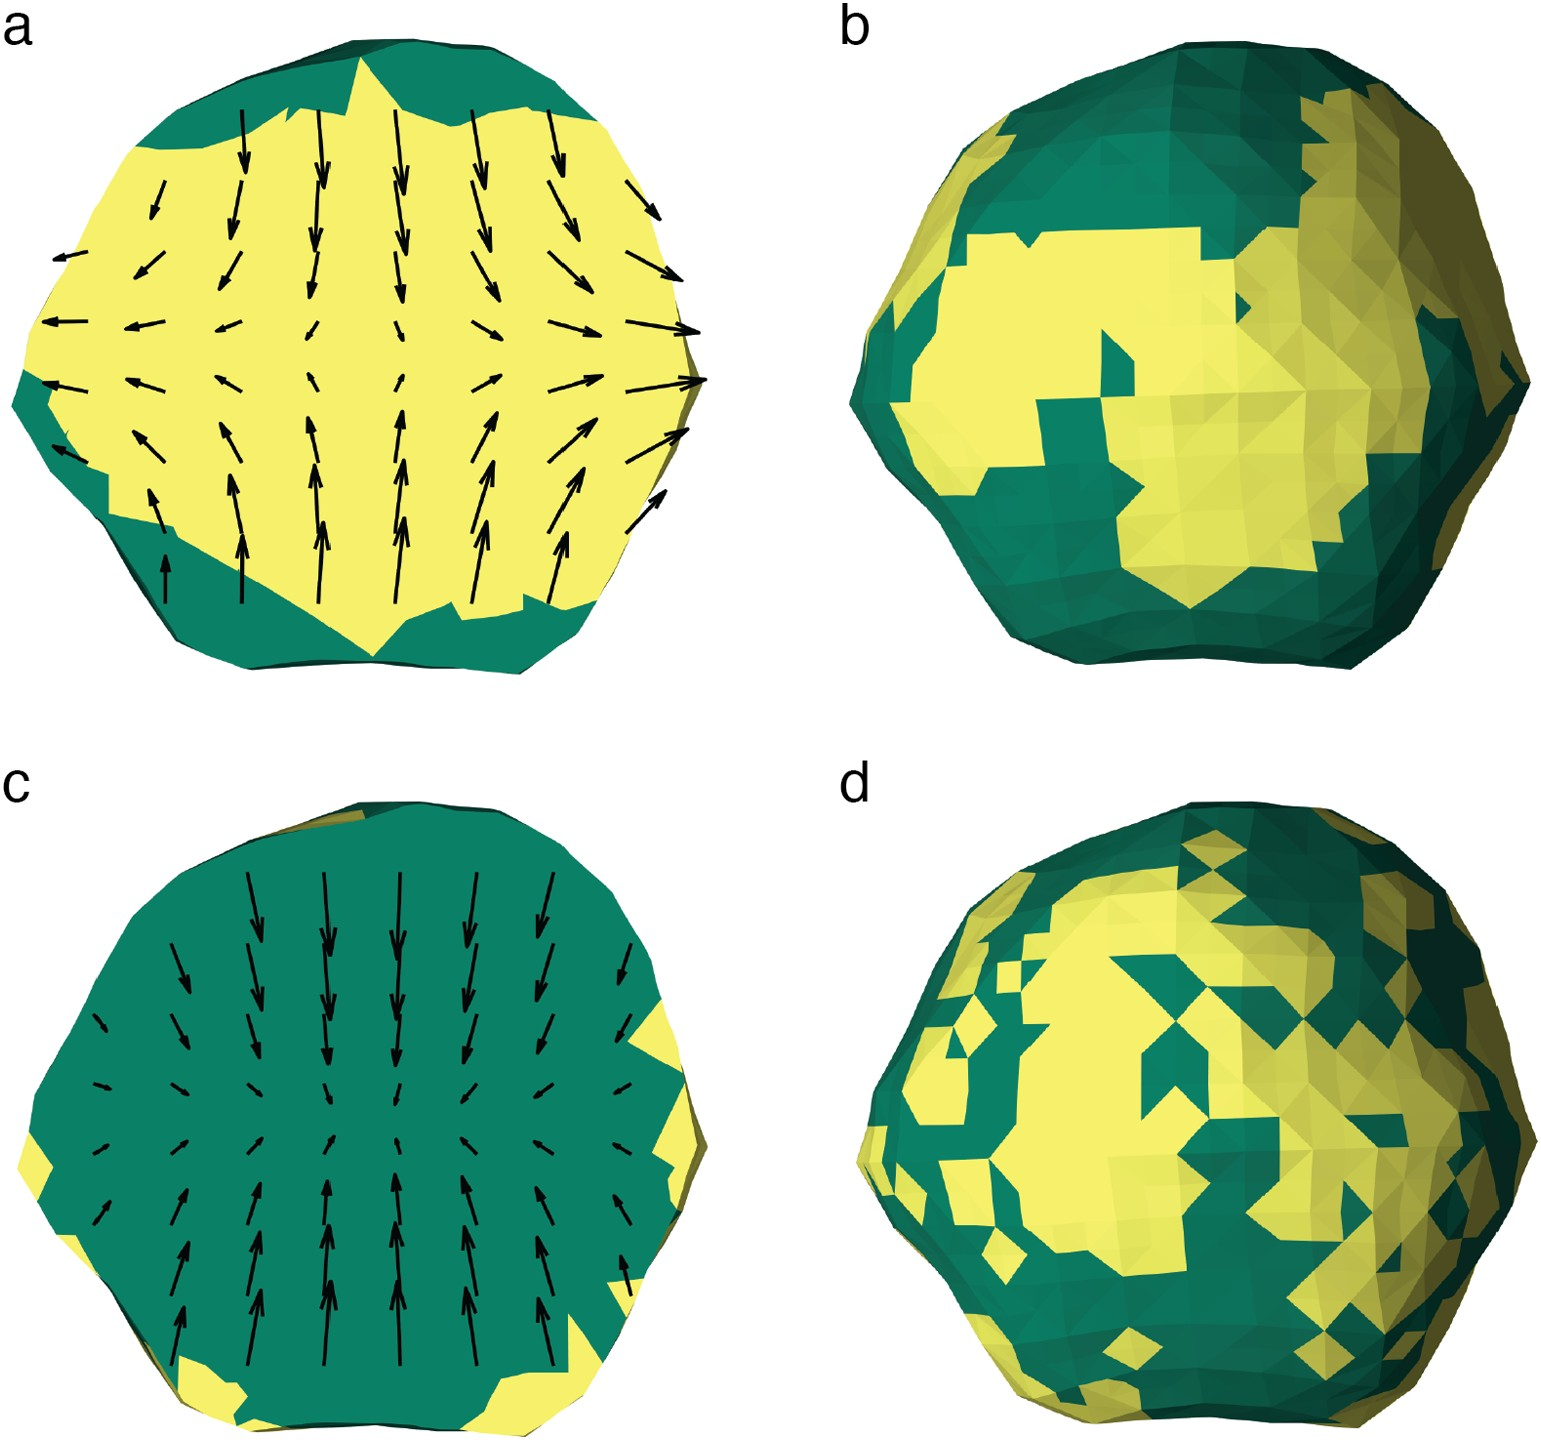
\includegraphics[scale=0.6]{figure/failure_models.jpg}
    \caption[Soluzioni dei modelli di cedimento basati sull'analisi di Didymos.]{Soluzioni dei modelli di cedimento basati sull'analisi di Didymos. Le figure $a$ e $b$ mostrano la soluzione nel caso di un periodo di rotazione di 2.26 h; $c$ e $d$ il caso con un periodo di 3.5 h. Le frecce sono indicano i vettori di deformazione. \citep{naidu_radar_2020}}
    \label{fig:failure_models}
\end{figure}

Una rotazione rapida contribuisce alla formazione di un asteroide top-shaped e lavori precedenti \citep{walsh_rotational_2008, walsh_spin-up_2012} hanno ipotizzato che sia frane che deformazioni interne possono portare alla formazione di un crinale equatoriale. Al momento non è possibile identificare quale sia stata la causa della formazione del rigonfiamento, ma lavori futuri che analizzeranno i dati raccolti da DART, LICIACube e Hera potranno fare chiarezza su questo aspetto. In particolare, immagini dettagliate della morfologia superficiale di Didymos potranno essere usate per determinare come la deformazione avviene in un ambiente di microgravità e per fornire vincoli alla struttura interna dell'asteroide.

\subsection{Asteroidi rubble-pile}
I modelli ottenuti utilizzando i dati delle osservazioni descritte nella \cref{sec:binary_system} hanno suggerito che la maggioranza degli asteroidi tra $\sim 0.2$ e $10\,km$ siano probabilmente rubble-pile. In consistenza con queste aspettative, gli asteroidi Itokawa ($0.3\,km$), Bennu ($0.5\,km$) e Ryugu ($0.9\,km$) sembrano essere rubble-pile. Per di più, il confronto dei massi più grandi con i crateri più larghi ha rivelato che la popolazione di rocce grandi è stata ereditata dalla distruzione catastrofica di un corpo progenitore \citep{DellaGiustina2019}.\\
Una recente analisi dei campioni recuperati dalla superficie di Ryugu ha rilevato come la densità del materiale di cui sono fatti i campioni sia simile alla densità globale dell'asteroide, indicando un'alta microporosità e una bassa macroporosità \citep{pilorget_first_2021}. Ciò è in contrasto con Itokawa, dove la macroporosità è alta e la microporosità bassa \citep{tsuchiyama_three-dimensional_2014}.\\
Questi risultati indicano la possibilità di un forte contrasto tra le caratteristiche della porosità interna di asteroidi appartenenti a diverse classi tassonomiche e ha implicazioni importati per quanto riguarda Didymos e Dimorphos. È anzi probabile che Didymos, con la sua forma e la rapida rotazione, sia un oggetto rubble-pile formatosi da una collisione \citep{zhang_creep_2021}. %\#\#\#Inoltre, analizzando qualitativamente le immagini, immortalate da LICIACube, dello scontro tra DART e Dimorphos, si potrebbe dedurre che anche il secondario sia di tipo rubble-pile. Saranno però necessari studi approfonditi che verranno pubblicati nel prossimo futuro.\#\#\#

\subsection{Indizi sulla formazione ed evoluzione del sistema}
È importante sottolineare che le condizioni geologiche osservate su Didymos e Dimorphos potrebbero correlare direttamente con i meccanismi di formazione ed evoluzione del sistema, quali: forze mareali, impatto, effetto rotazionale del primario, luna originale di un corpo progenitore.\\
Prendendo in considerazione gli attuali dati radar \citep{naidu_radar_2020} e le curve di luce \citep{pravec_binary_2016}, è possibile escludere le forze mareali come meccanismo rilevante per la formazione ed evoluzione di Dimorphos. Infatti, le forze mareali fanno sì che il corpo precursore si deformi in un corpo allungato. Al contrario, secondo i modelli descritti nella \cref{sec:shape_model}, Didymos è pressoché assisimmetrico, in contraddizione con la forma attesa dovuta alle forze mareali. Le curve di luce più recenti suggeriscono un oggetto leggermente più piccolo, più sferico e più denso \citep{pravec_photometric_2022}.\\
Per quanto riguarda lo scenario dell'impatto, l'esistenza di grandi crateri su Didymos potrebbero esserne un potenziale indicatore. Nell'eventualità che Didymos si riveli essere monolitico, questo scenario è escluso perché per formare un corpo delle dimensioni di Dimorphos servirebbe un impatto che genererebbe un cratere di 10 km di diametro, molto più grande rispetto alla dimensione del primario. Nel caso di un impatto sub-catastrofico, invece, potrebbe non esserci un'evidenza univoca di crateri. Una grande quantità di materia potrebbe essere espulsa da Didymos a basse velocità contribuendo alla formazione ed evoluzione del satellite. In questo caso Didymos presenterebbe numerose caratteristiche topografiche asimmetriche: sarebbe possibile, quindi, trovare materiale esogeno sulla superficie dell'asteroide.\\
%Il periodo di rotazione potrebbe essere abbastanza breve da indurre un rimodellamento su varie scale di lunghezza: da movimenti di massa in zone confinate della superficie a una riconfigurazione globale. \\

Lo scenario dell'effetto rotazionale deriva dalle espulsioni di massa dovute al breve periodo di rotazione. In questo caso, in base alla presenza di coesione, la formazione di Dimorphos potrebbe essere differente. Se c'è coesione, una roccia monolitica potrebbe aver lasciato Didymos. Non è ancora chiaro quale potrebbe essere il lascito di questo evento, dato che sui piccoli asteroidi i massi più grandi sono ben sepolti e non si muovono facilmente \citep{daly_hemispherical_2020}. Se le particelle non sono coese, la perdita di materiale dalla superficie e la sua successiva riaccumulazione potrebbero portare alla formazione di un satellite \citep{walsh_spin-up_2012}. Per lo scenario senza coesione, i due asteroidi avrebbero la stessa composizione, ma la presenza di regolite fine ($<1\,cm$) potrebbe essere differente. La pressione di radiazione solare potrebbe aver avuto abbastanza tempo per spazzare via le particelle più piccole. Inoltre, l'evoluzione orbitale degli ejecta, da Didymos a Dimorphos, potrebbe portare a essere più giovane la faccia di Dimorphos rivolta verso Didymos, essendo il secondario sincronizzato marealmente con il primario e gli ejecta affetti da SW con un tasso minore \citep{agrusa_excited_2021}.

La geologia superficiale potrebbe anche dipendere dall'evoluzione delle orbite tra Didymos e Dimorphos. Per esempio, l'accelerazione dell'anomalia media di Dimorphos è stata calcolata essere bassa, il che fa propendere per due possibili scenari. Per quanto riguarda il primo, se questa bassa accelerazione dell'anomalia media è dovuta al moto caotico di Dimorphos, l'accumulo di materiale potrebbe essere uniforme sulla superficie rivolta verso Didymos. In questo scenario, il riscontro geologico sarebbe trovare materiale di età simile su tutta la superficie di Dimorphos. Il secondo scenario è che nonostante l'effetto BYORP sia significativo questo venga cancellato dalle forze mareali del primario sul secondario. In questo caso, una faccia di Dimorphos sarebbe sempre rivolta verso il primario, portando a una dicotomia nei colori delle due facce, poiché il materiale proveniente da Didymos si depositerebbe solo sulla faccia rivolta verso di esso.

\section{Caratteristiche spettrali pre-impatto}
Adottando un diametro di Didymos di $D_p=0.75 \pm 0.1\; km$, dalle stime delle immagini delay-Doppler ottenute con il telescopio di Arecibo, si ottiene un'albedo geometrica nel visibile di $p_V=0.16 \pm 0.04$, valore congruente con quello trovato successivamente da \citet{naidu_radar_2020} utilizzando gli stessi dati grezzi. \citet{binzel_observed_2004} ha classificato l'asteroide come Xk nella tassonomia di Bus. Dunque, sommando le informazioni della classificazione con quelle dell'albedo, l'asteroide è classificato come classe M nella tassonomia di Tholen.\\
Con le successive apparizioni, tra il 2003 e il 2019, sono state svolte ulteriori osservazioni spettroscopiche, ma la classificazione di Didymos è rimasta enigmatica. In seguito al lavoro di \citet{binzel_observed_2004}, \citet{de_leon_spectral_2006, de_leon_observations_2010} ha esteso la tassonomia nel vicino infrarosso e ha classificato l'asteroide come potenziale tipo S. \citet{dunn_mineralogies_2013} ha confermato che Didymos sembra spettroscopicamente consistente con le condriti ordinarie, con un'affinità per le meteoriti di tipo L/LL. Nel corso del tempo è maturato il consenso che Didymos sia composto da silicati, anche se rimangono alcune anomalie come quella della banda a $2\,\mu m$ che appare meno profonda rispetto a quella dei tipici asteroidi silicatici. 

La campagna osservativa svolta da \citet{ieva_spectral_2022} con il Telescopio Nazionale Galileo (TNG) nel 2021, ha confermato la natura silicatica con qualche discrepanza. L'analisi degli spettri, confrontati con quelli d'archivio e gli spettri delle meteoriti all'interno del database RELAB\footnote{\href{https://pds-speclib.rsl.wustl.edu/search.aspx?catalog=RELAB}{https://pds-speclib.rsl.wustl.edu/search.aspx?catalog=RELAB}}, ha mostrato una variazione tenue ma persistente della pendenza spettrale del sistema di Didymos, tra $0.5$ e $0.7\,\mu m$. 

\begin{figure}[!h]
    \centering
    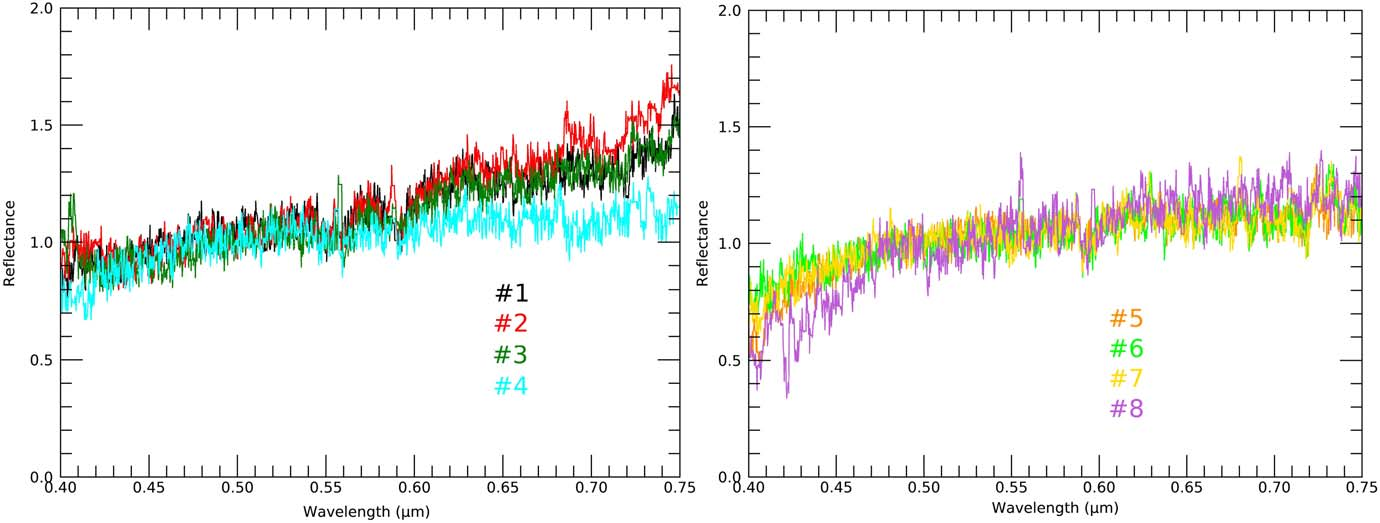
\includegraphics[scale=0.65]{figure/spettri_tot_ieva.jpg}
    \caption[Spettri osservati con il TNG durante l'apparizione del 2021.]{Tutti gli spettri osservati con il TNG durante l'apparizione del 2021. Gli spettri 1-7 sono stati osservati durante la notte del 15 febbraio, mentre lo spettro 8 è stato osservato il 23 febbraio. Tutti gli spettri sono normalizzati a $0.55\,\mu m$. \citep{ieva_spectral_2022}}
    \label{fig:spettri_tot_ieva}
\end{figure}

La variazione, in principio, potrebbe essere dovuta al contributo del secondario, ma Dimorphos, essendo circa un quinto della dimensione del primario, dovrebbe contribuire solo al 4\% della luce osservata, assumendo albedo e composizione simili al primario. Eventuali differenze spettrali per essere rilevate dovrebbero essere dovute a caratteristiche enormemente differenti, anche perché il sistema al momento delle osservazioni era molto debole (V=18.0). Tuttavia, gli spettri raccolti subito prima, durante e subito dopo un'eclissi del primario mostrano una pendenza notevolmente omogenea, indicando potenzialmente una somiglianza tra il primario e il secondario. Questa evidenza, insieme al fatto che il contributo di Dimorphos in questi spettri dovrebbe essere minimale, potrebbe significare che le differenze osservate nel comportamento spettrale non sono dovute a disomogeneità del secondario rispetto al primario.

\begin{figure}[!h]
    \centering
    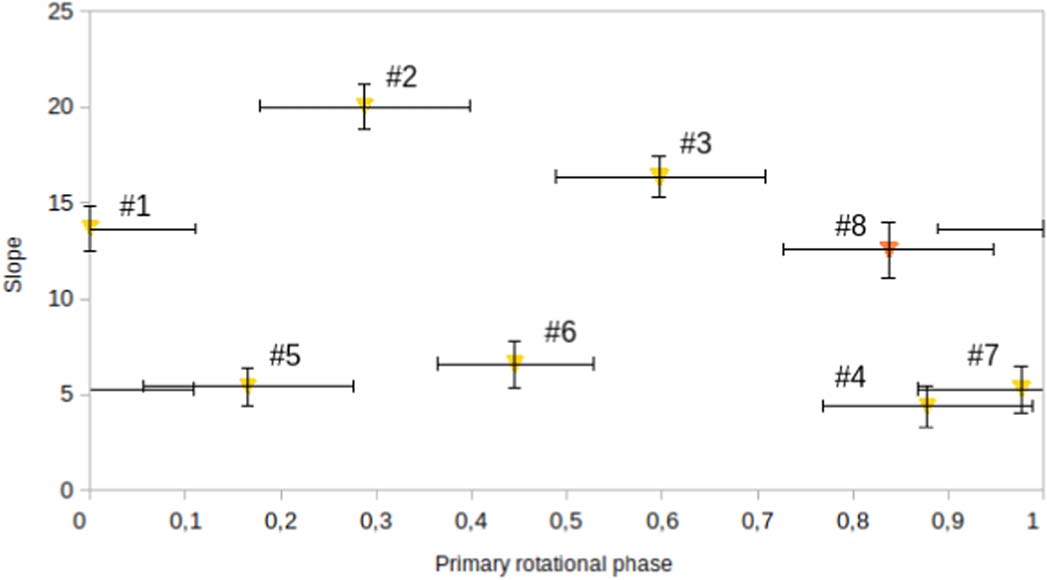
\includegraphics[scale=0.7]{figure/slope_ieva.jpg}
    \caption[Pendenze spettrali dei dati del 2021.]{Pendenze spettrali ricavate dai dati del 2021 vs la frazione di fase rotazionale, assegnata prendendo il primo spettro come riferimento. Gli spettri osservati durante il 15 febbraio sono in giallo, quello osservato il 23 febbraio in arancione. \citep{ieva_spectral_2022}}
    \label{fig:slope_ieva}
\end{figure}

L'analisi mostra che gli spettri (e.g. \#4, \#5, \#7) con una pendenza simile potrebbero riferirsi alla stessa regione sulla superficie di Didymos (se l'oggetto fosse invece omogeneo, potrebbero avere pendenze simili in regioni diverse). Al contrario, alcuni spettri (e.g. \#1, \#7) centrati alla stessa fase di rotazione mostrano una grande differenza nella pendenza spettrale. È importante ricordare che le osservazioni da terra sono \textit{disk integrated}, aspetto che non può escludere la presenza variegazioni superficiali più o meno estese.

\begin{figure}[!h]
    \centering
    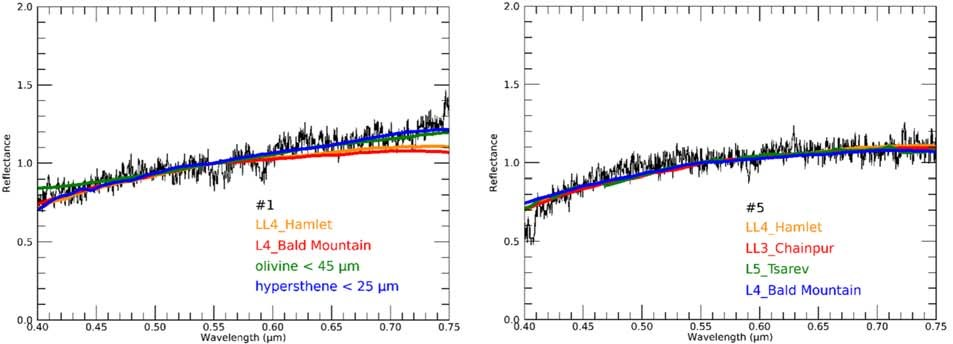
\includegraphics[scale=0.96]{figure/Ieva et al.jpg}
    \caption[Confronto tra spettri di Didymos e analoghi delle meteoriti.]{Confronto tra due spettri di Didymos, ottenuti durante l'osservazione del sistema con il TNG nel 2021, e quelli dei migliori analoghi delle meteoriti, selezionate attraverso il tool M4AST (per approfondire consigliamo \cite{popescu_modelling_2012}). Il tool è stato usato per confrontare i dati con quelli presenti nel database RELAB, selezionando quelli con il minor $\chi^2$. \citep{ieva_spectral_2022}}
    \label{fig:ieva_spectra}
\end{figure}

In conclusione, il confronto con il database RELAB conferma una somiglianza generale tra Didymos e le condriti ordinarie di tipo L/LL. Tuttavia, gli spettri più ripidi possono essere dovuti alla presenza di iperstene e/o olivina, principali componenti delle condriti di tipo L (\cref{fig:ieva_spectra}).

\begin{table}[!h]
    \begin{center}
    \resizebox{\linewidth}{!}{%
      \begin{tabular}{ccc}
      \toprule
      \toprule
      Parametro &       & Valore \\
      \midrule
      Sistema: &       &  \\
      Mag assoluta & $H_V$ & $18.16\pm 0.04$ \\
      Albedo geometrica (VIS) & $p_V$ & $0.16\pm 0.04$ \\
      Classe tassonomica &       & S \\
      \midrule
      Primario: &       &  \\
      Diametro equivalente & $D_1\;(km)$ & $0.780\pm 0.030$ \\
      Periodo di rotazione & $P_1\;(h)$ & $2.2600\pm 0.0001$ \\
      Densità globale & $\rho_1\;(g\,cm^{-3})$ & $2.17\pm 0.35$ \\
      \midrule
      Secondario: &       &  \\
      Diametro equivalente & $D_2\;(km)$ & $0.171\pm 0.011$ \\
      \midrule
      Orbita del sistema: &       &  \\
      Semiasse maggiore & $a\;(km)$ & $1.19\pm 0.03$ \\
      Deriva dell'anomalia media & $\Delta M_d\;(deg\,yr^{-2})$ & $0.15\pm 0.14$ \\
      Periodo orbitale a $t_0$ & $P_{orb}\;(h)$ & $11.921624\pm 0.000018$ \\
      Eccentricità & $e$   & $\leq 0.03$ \\
      Epoca & $t_0$ & JD 2,455,873.0 (asterocentric UTC) \\
      \bottomrule
	  \bottomrule
      \end{tabular}}%
    \end{center}
    \caption{Riassunto dei principali parametri dinamici, morfologici e dinamici del sistema di (65803) Didymos pre-impatto.}  
    \label{tab:param_didymos}%
  \end{table}%
  

\section{Didymos come obiettivo della missione DART}
La scelta di Didymos si è basata su due aspetti principali: quello ingegneristico e quello del ritorno scientifico.\\
Essendo un sistema binario era il candidato perfetto per condurre il test dell'impattatore cinetico con una sola sonda, confrontando prima e dopo l'orbita del secondario (operazione che può essere svolta per via spettrofotometrica). Inoltre tra i circa 60 NEA binari, il sistema di Didymos aveva un $\Delta V$ (parametro legato all'energia necessaria per raggiungere un oggetto nello spazio) che lo rendeva il più accessibile tra tutti in termini di costi-benefici. Il sistema è stato scelto anche perché l'orbita di Didymos non interseca quella terrestre e l'impatto sulla luna Dimorphos non pone alcun pericolo alla sicurezza della Terra. Selezionando Dimorphos si è scelto un oggetto di più di 100 metri di diametro e quindi paragonabile agli asteroidi catalogati come PHA.\\
Dal punto di vista di ritorno scientifico, Didymos è stato selezionato perché è un sistema binario a eclissi il che permette di fare misure accurate nel caso di piccole variazioni del periodo orbitale del secondario, sia dalla Terra che dallo spazio. In aggiunta, il sistema a settembre 2022 era alla minima distanza con la Terra, e in opposizione, massimizzando l'efficacia delle osservazioni spettrofotometriche.\\
In più lo studio di un sistema binario, prima, durante e dopo la missione DART, insieme alla approfondita campagna di osservazioni in situ che verrà svolta con la missione Hera, permetterà di gettare luce sui vari problemi ancora irrisolti discussi nei capitoli precedenti.

\begin{figure}[!h]
    \centering
    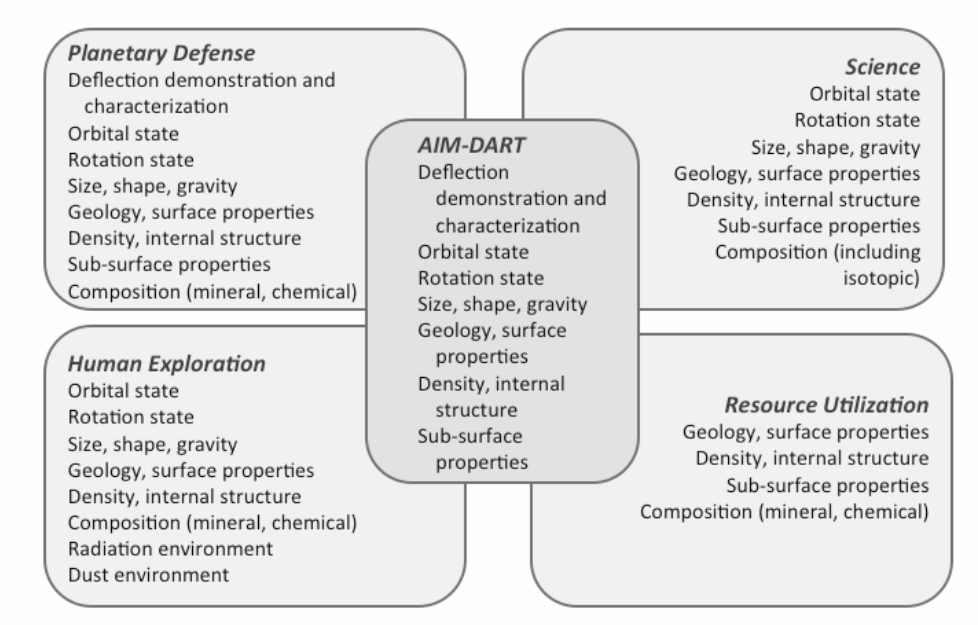
\includegraphics[width=\textwidth]{figure/Michel et al.png}
    \caption[Riassunto del ritorno scientifico e tecnologico dovuto alle missioni DART e Hera.]{Riassunto del ritorno scientifico e tecnologico dovuto alle missioni DART e Hera. \citep{MICHEL20162529}}
    \label{fig:ritorno_scientifico}
\end{figure}

\chapter{Risultati preliminari post-impatto}\label{ch:ch_5}
Al momento della scrittura di questa tesi, alcuni lavori con i primissimi risultati sono stati da poco sottomessi alle maggiori riviste scientifiche internazionali e per questo motivo possiamo basarci solo sui comunicati stampa che NASA e il team di DART hanno pubblicato poche settimane dopo lo scontro di DART con Dimorphos, contenenti alcuni risultati preliminari ottenuti con diversi degli osservatòri mostrati in \cref{fig:obs_dart}. 

\section{Risultati NASA}
Dallo spazio, i telescopi James Webb Space Telescope (JWST) e Hubble Space Telescope (HST) hanno operato in sinergia per osservare il sistema di Didymos poco prima e dopo l'impatto. Le osservazioni di JWST e HST permetteranno ai gruppi di ricerca di ricavare informazioni sulla natura della superficie di Dimorphos, sulla quantità di materiale espulso dalla collisione e sulla sua velocità. Inoltre, Webb e Hubble hanno osservato l'impatto a diverse lunghezze d'onda: Webb nell'infrarosso e Hubble nel visibile. L'osservazione dell'impatto in un'ampia gamma di lunghezze d'onda permetterà di rivelare la distribuzione delle dimensioni delle particelle nella nube di polvere in espansione, aiutando a determinare se l'impatto ha espulso pezzi grandi o soprattutto polvere fine. 

\begin{figure}[!h]
    \centering
    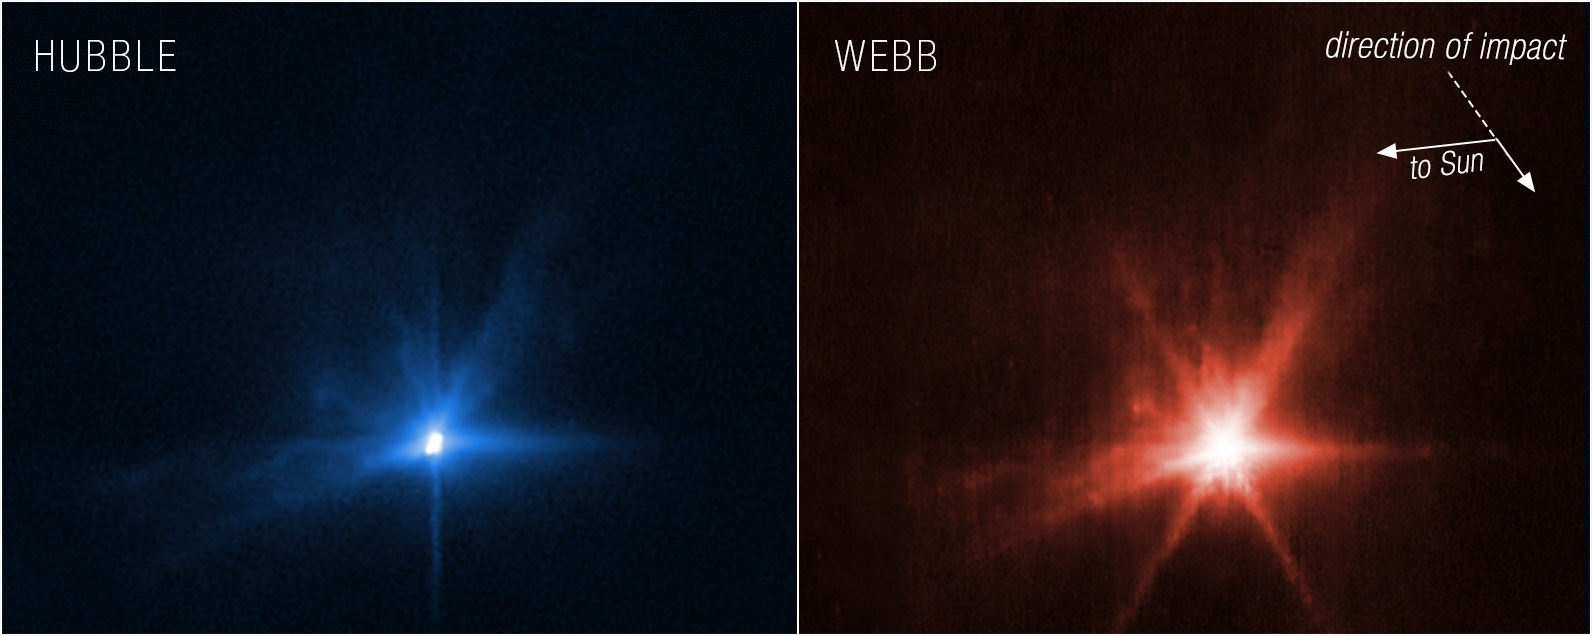
\includegraphics[width=\textwidth]{figure/jwst_hst_impact.png}
    \caption[Immagini catturate da Hubble e da Webb diverse ore dopo l'impatto di DART con Dimorphos.]{Immagini catturate da HST (sinistra) e da JWST (destra) diverse ore dopo l'impatto di DART con Dimorphos. (NASA/ESA/CSA/STScI)}
    \label{fig:jwst_hst_impact}
\end{figure}

\paragraph*{Osservazioni con il JWST}
Il James Webb ha effettuato un'osservazione del sistema prima che avvenisse la collisione, poi diverse osservazioni nelle ore successive. Le immagini della NIRCam (Near-Infrared Camera) di Webb mostrano un nucleo compatto, con pennacchi di materiale che si allontanano dal centro del punto in cui è avvenuto l'impatto (\cref{fig:jwst_hst_impact}).\\
L'osservazione dell'impatto con il JWST non è stata semplice a causa della velocità di spostamento dell'asteroide nel cielo. Per questo motivo, nelle settimane precedenti l'impatto, i team a terra hanno messo a punto e testato un metodo di tracciamento per gli asteroidi che si muovono a una velocità tre volte superiore al limite di velocità originariamente fissato.\\
I team prevedono di osservare il sistema anche nei prossimi mesi utilizzando lo strumento per il medio infrarosso (MIRI) e lo spettrografo che lavora nel vicino infrarosso (NIRSpec). I dati spettroscopici forniranno ai ricercatori informazioni sulla composizione chimica dell'asteroide.

\paragraph*{Osservazioni con l'HST}
Anche Hubble ha osservato il sistema binario prima dell'impatto e poi 15 minuti dopo che DART ha colpito la superficie di Dimorphos. Le immagini della Wide Field Camera 3 (WFC3) di Hubble mostrano l'impatto in luce visibile (\cref{fig:jwst_hst_impact,fig:hst_plume}).\\
Il flusso di ejecta più vistoso, in basso a sinistra rispetto all'asteroide, si trova nella direzione da cui si è avvicinata DART. Alcuni dei pennacchi sembrano essere leggermente curvati, ma una spiegazione accurata richiederà ulteriori analisi approfondite. Dalle immagini di Hubble si è stimato che la luminosità del sistema sia aumentata di tre volte dopo l'impatto e che sia rimasta costante anche otto ore dopo l'impatto.\\
Hubble ha osservato il sistema altre 10 volte nelle tre settimane successive l'impatto. Queste osservazioni a lungo termine, mentre la nube di ejecta si espande e si affievolisce, forniranno un quadro più completo sull'espansione della nube, dall'espulsione dei materiali alla sua scomparsa.

\paragraph*{Osservazioni fotometriche}
Le analisi preliminari dei dati, fotometrici e radar, ottenuti nelle settimane successive all'impatto mostrano che questo ha, con molta probabilità, alterato l'orbita dell'asteroide.\\
Prima dell'impatto di DART, Dimorphos aveva un periodo orbitale di 11 ore e 55 minuti. Utilizzando vari telescopi terrestri, il team di DART ha misurato una variazione del periodo, osservando nei dati fotometrici ogni quanto Dimorphos eclissava Didymos (\cref{fig:impact_lightcurve}). Il team ha confermato che la variazione del periodo orbitale pare essere di 32 minuti, accorciando l'orbita a 11 ore e 23 minuti. Questa misura ha un margine di incertezza di circa 2 minuti. 
Il team scientifico della missione aveva previsto un cambiamento di 73 secondi o più. Questi primi dati mostrano che DART ha superato questo valore minimo di oltre 25 volte. \\

Il team sta ancora acquisendo dati con osservatòri in tutto il mondo, oltre che con le strutture radar del Goldstone Planetary Radar del Jet Propulsion Laboratory della NASA in California e del Green Bank Observatory della National Science Foundation in West Virginia (\cref{fig:expected_dimorphos}), con lo scopo di migliorare la precisione di misurazione del periodo.

L'attenzione si sta ora spostando verso la misurazione dell'efficienza del trasferimento di quantità di moto a seguito della collisione di DART con il suo bersaglio, avvenuta a circa 22.530 chilometri all'ora. Ciò include un'ulteriore analisi degli ejecta, poiché il contraccolpo di questa espulsione di detriti ha potenzialmente aumentato in modo sostanziale la spinta di DART contro Dimorphos. %- un po' come un getto d'aria che esce da un palloncino lo manda nella direzione opposta.
Per comprendere appieno questo effetto sono necessarie ulteriori informazioni sulle proprietà fisiche dell'asteroide, come le caratteristiche della sua superficie, le proprietà strutturali e la coesione tra particelle. Questi aspetti sono ancora in fase di studio.\\
Per questa analisi sarà necessario studiare le immagini di Dimorphos scattate da DART e LICIACube durante l'avvicinamento (e.g. \cref{fig:liciacube_impact_1,fig:liciacube_impact_tot}), per stimare la massa e la forma dell'asteroide. Una caratterizzazione morfologica e geologica più completa sarà fornita dalla missione Hera, di cui si è parlto brevemente nella \cref{sec:hera}.

\begin{figure}
    \centering
    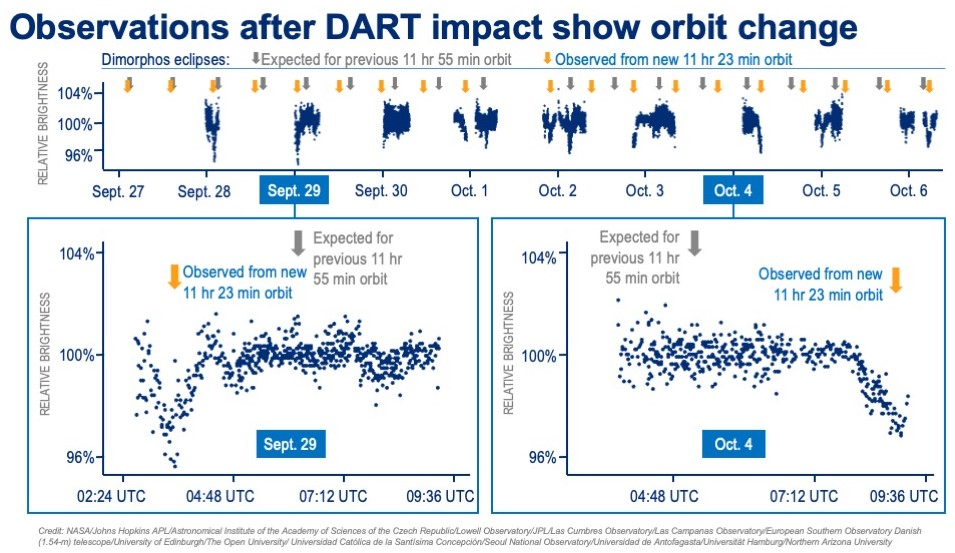
\includegraphics[width=\textwidth]{figure/impact_lightcurve.jpg}
    \caption[Riassunto dei dati fotometrici utilizzati per determinare l'orbita post-impatto.]{I grafici offrono un riassunto dei dati fotometrici che il team di DART ha utilizzato per determinare l'orbita di Dimorphos dopo l'impatto, grazie alle piccole diminuzioni di brillanza dovute alle eclissi reciproche tra Didymos e Dimorphos. I dati mostrano che le eclissi sono avvenute a un orario diverso (frecce arancioni) rispetto alle previsioni in cui il periodo orbitale rimane invariato (frecce grige). Le nuove diminuzioni di luminosità avvengono ogni 11 ore e 23 minuti, una diminuzione di 32 minuti rispetto al periodo orbitale pre-impatto di 11h 55m. (NASA/JHU-APL)}
    \label{fig:impact_lightcurve}
\end{figure}

\begin{figure}
    \centering
    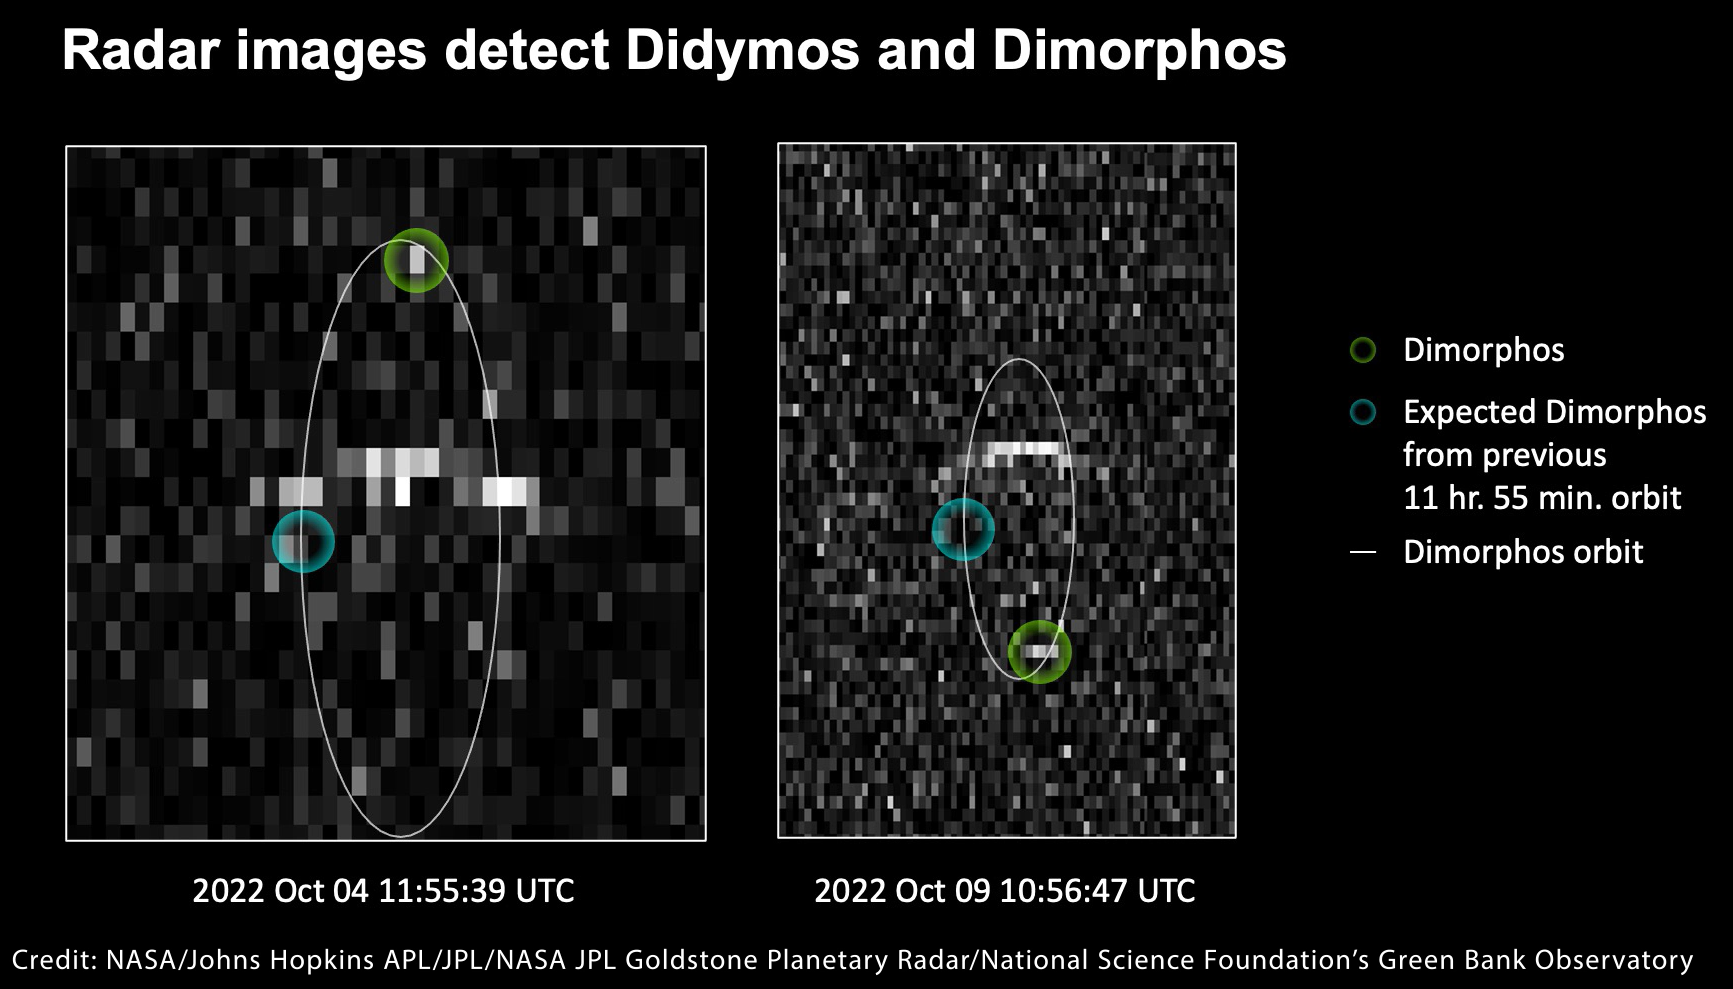
\includegraphics[scale=0.25]{figure/expected_dimorphos.png}
    \caption[Immagine radar del sistema post-impatto.]{Immagine radar del sistema binario ottenuta dall'osservatorio di Goldstone (GO) e dal Green Bank Observatory (GBO). A sinistra osservazioni fatte il 4 ottobre fatte dal GO, a destra le osservazioni combinate di GO e GBO fatte il 9 ottobre. Sull'asse verticale la distanza con la Terra, su quello orizzontale la frequenza Doppler. Il cerchio azzurro mostra la posizione attesa se non ci fosse stata una variazione del periodo orbitale, il cerchio verde mostra la posizione effettiva di Dimorphos. (Crediti nell'immagine)}
    \label{fig:expected_dimorphos}
\end{figure}

\section{Osservazioni da Asiago}
Durante le notti del 17, 18, 19 ottobre ho contribuito a raccogliere gli spettri del sistema di Didymos con il telescopio Copernico dell'Osservatorio Astrofisico di Asiago. I dati sono al momento in fase di elaborazione e di confronto con quelli raccolti dagli altri team di DART.\\
I dati raccolti ad Asiago andranno ridotti con estrema cura per poter escludere qualsiasi tipo di bias dovuto alle condizioni di osservazione non ottimali. Infatti, oltre alle condizioni meteo non ideali, il telescopio ha avuto dei problemi con l'inseguimento dell'asteroide, causando l'uscita dalla fenditura prima che il tempo di posa fosse terminato. Oltre a ciò, gli spettri di Didymos sono stati presi sotto un valore di airmass\footnote{È la misura della quantità di aria lungo la linea di vista quando un oggetto celeste è osservato da Terra. In approssimazione piano-parallela dell'atmosfera, a un angolo zenitale di 60° l'airmass è circa 2.} elevato, dal momento che l'oggetto si trovava a un'altezza non superiore ai 40° per tutto l'arco osservativo.\\
Al momento, quindi, non c'è un risultato certo sulla composizione dei due asteroidi. Quando saranno disponibili, queste informazioni, complementari a quelle fotometriche e radar, saranno essenziali per migliorare la comprensione del sistema e le conseguenze dell'impatto.


\begin{figure}
    \centering
    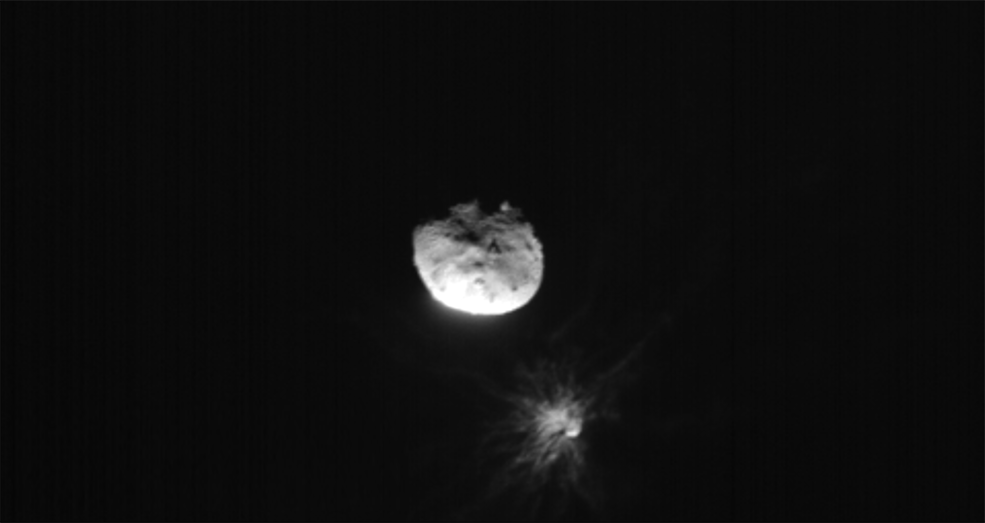
\includegraphics[width=\textwidth]{figure/liciacube_impact_1.png}
    \caption[Immagine scattata da LICIACube poco prima del flyby con Dimorphos.]{Immagine scattata da LICIACube poco prima del flyby con Dimorphos. Si vedono distintamente Didymos, Dimorphos e la nube di detriti generata dall'impatto. (ASI/NASA)}
    \label{fig:liciacube_impact_1}
\end{figure}

\begin{figure}
    \centering
    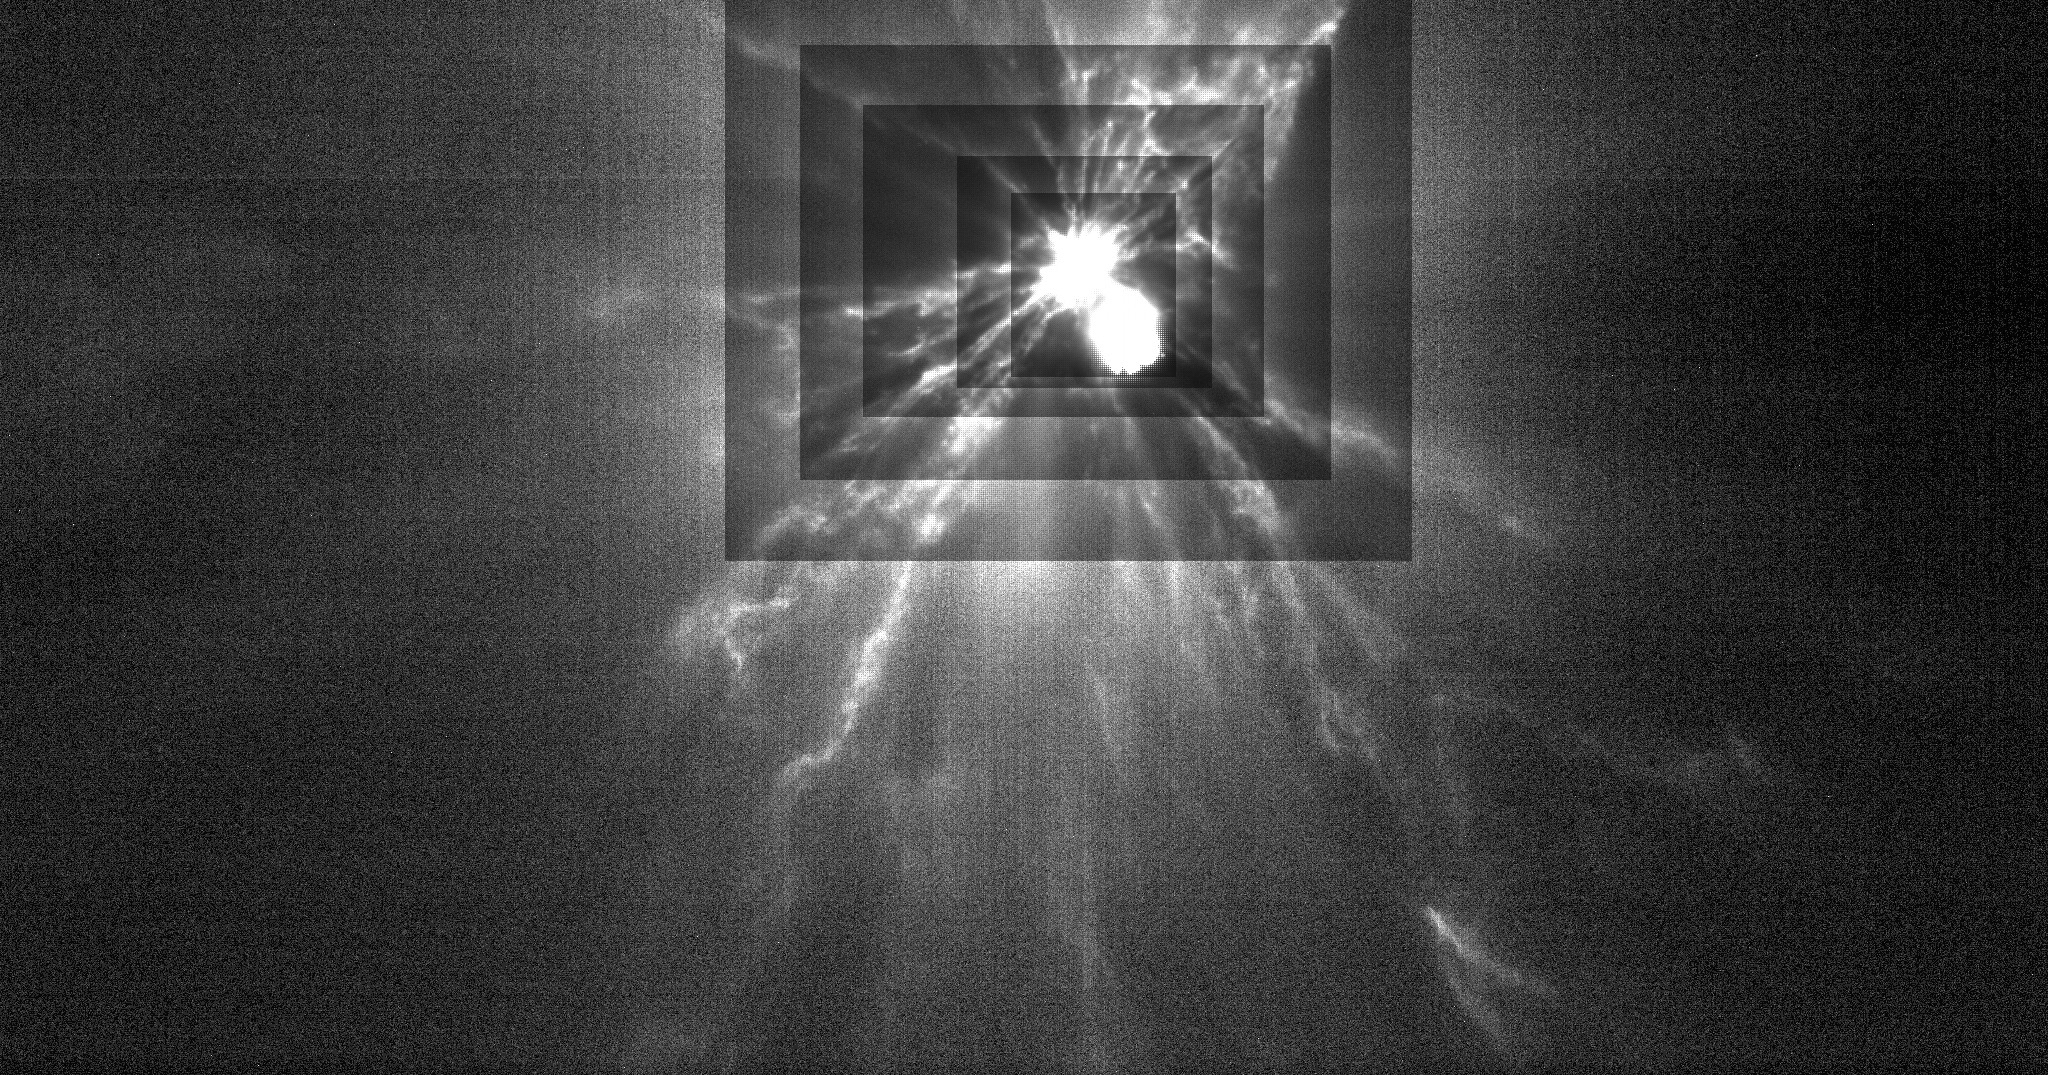
\includegraphics[width=\textwidth]{figure/liciacube_impact_tot.jpg}
    \caption[Immagine ottenuta da LICIACube dopo il flyby con Dimorphos.]{Immagine ottenuta da LICIACube dopo il flyby con Dimorphos. Ogni riquadro rappresenta un diverso livello di contrasto per mettere in risalto la struttura fine dei pennacchi di detriti. Studiando questi pennacchi si sarà in grado di approfondire le conoscenze sugli asteroidi e i processi di impatto. (ASI/NASA/APL)}
    \label{fig:liciacube_impact_tot}
\end{figure}

\begin{figure}
    \centering
    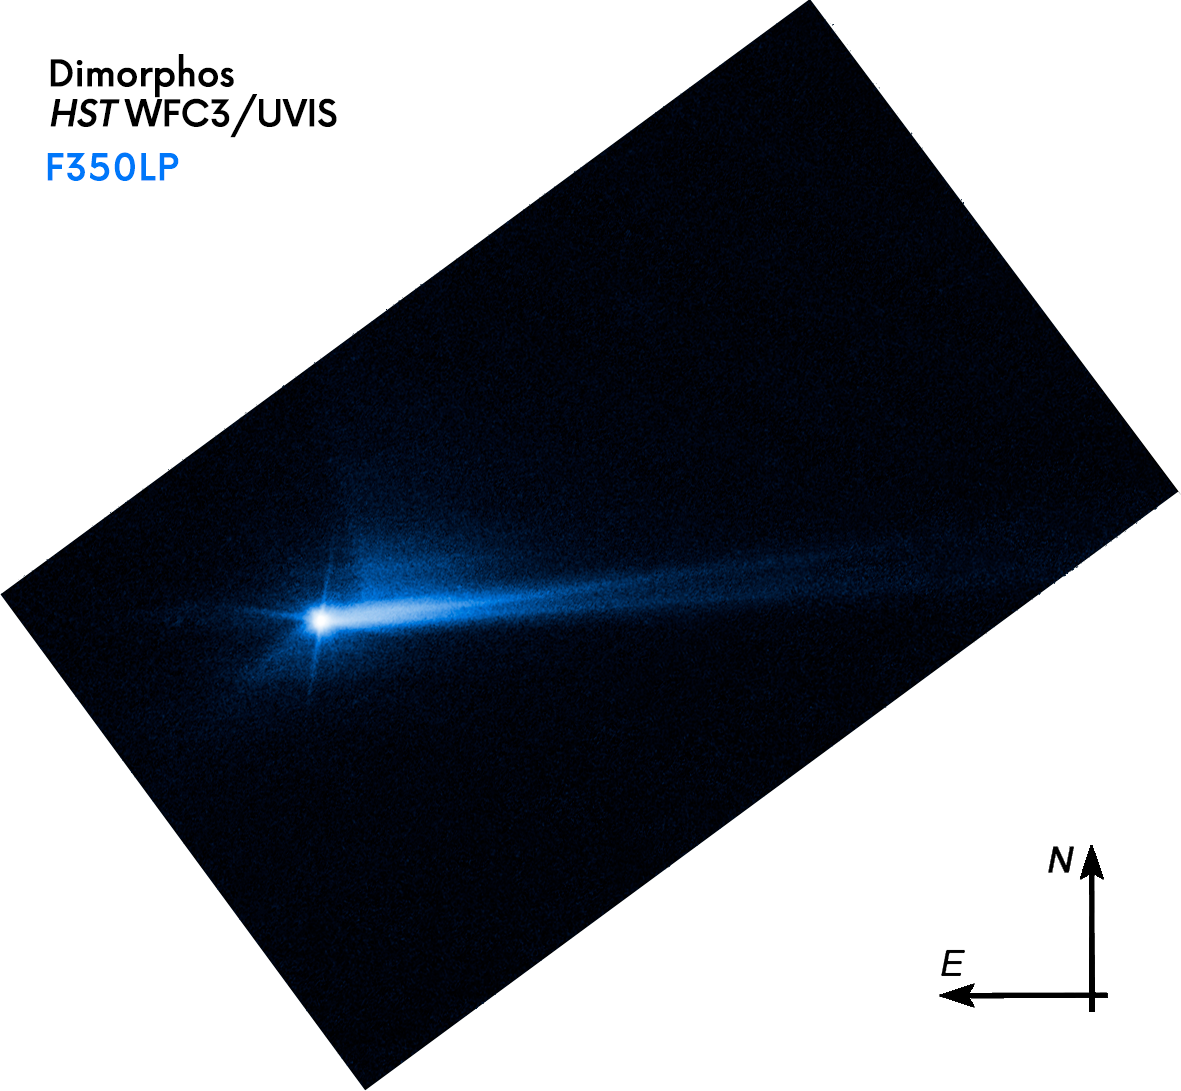
\includegraphics[scale=0.25]{figure/hst_plume.png}
    \caption[Immagine della coda di detriti scattata da HST.]{Immagine scattata dal telescopio spaziale Hubble l'8 ottobre 2022. Si nota chiaramente la coda di detriti che si estende per più di 10000 km. (NASA/ESA/STScI/HST)}
    \label{fig:hst_plume}
\end{figure}

\chapter*{Conclusioni}
\addcontentsline{toc}{chapter}{Conclusioni}
Che ce scrivo? BOOOOOOH

L'intensa campagna osservativa, iniziata dopo l'impatto, ha portato ai primi risultati preliminari, ottenuti tramite osservazioni fotometriche, che mostrano come l'impatto della sonda DART su Dimorphos abbia modificato l'orbita di quest'ultimo portando a una riduzione del periodo orbitale di $32 \pm 2$ minuti.\\
Continua la caratterizzazione spettroscopica del sistema da parte di vari telescopi terrestri e nello spazio. In particolare, nei prossimi mesi parteciperò alla riduzione e successiva analisi dei dati ottenuti dalle osservazioni, a cui ho collaborato, svolte nel mese di ottobre 2022 con il telescopio Copernico dell'Osservatorio Astrofisico di Asiago. Al momento, non essendo disponibili dati certi, non esiste un risultato certo sulla composizione del sistema. 

Nei prossimi mesi verranno pubblicati i primi articoli scientifici, che sono da poco stati sottomessi alle maggiori riviste scientifiche internazionali, fornendo i primi risultati sull'analisi del sistema binario Didymos, in attesa della futura missione Hera.


\cleardoublepage
\addcontentsline{toc}{chapter}{\bibname}
\printbibliography



\end{document}